\chapter{The ATLAS Detector}

\label{ch:atlas}
% --------------------------------------------------------------------------------

The four major \ac{LHC} experiments at \ac{CERN} seek to use the never before matched energies and luminosities of the new collider to explore the boundaries of particle physics and to gain insight into the fundamental forces of nature.
Two of these experiments, \ac{ATLAS} and \ac{CMS}, are general purpose detectors that seek to measure a variety of processes in the up to 14 \TeV proton-proton collisions that occur as much as 40 million times per second at the \ac{LHC} at the design luminosity of $10^{34}$ \lcms. 
\ac{ATLAS} employs a hermetic detector design, one which encloses the particle collisions as completely as possible with detecting elements, that allows it to study a wide range of physics from \ac{SM} and Higgs measurements to searches for new physics in models like \acl{SUSY}~\cite{atlas_experiment}.

Accomodating this wide variety of goals is a challenge for the design of the detector.
The wide range of energies involved requires high measurement precision over several orders of magnitude and the ability to measure a variety of particle types.
At the time of the construction of \ac{ATLAS}, the Higgs boson had yet to be discovered, but the diphoton decay mode was (correctly) expected to be important and necessitated a high resolution photon measurement.
The potential for decays of new heavy gauge bosons, W' and Z', required a similarly high momentum resolution for leptons with momentum up to several \TeV.
Hadronic decay modes of several possible new high energy particles could result in very energetic jets, again up to several \TeV, and reconstructing the decay resonances would again require good energy resolution.
Several models, such as \ac{SUSY} or Extra Dimensions, predict the existence of particles which would not interact with traditional detecting elements. 
However these particles can still be observed in a hermetic detector by accurately measuring the remaining event constituents to observe an imbalance in energy called missing energy or \met. 
Measuring \met implicity requires a good resolution on all \ac{SM} particles that can be produced.
And at the lower end of the energy spectrum, precision \ac{SM} measurements would require good resolution of a variety of particle types at energies as low as a few \GeV, so the design needs to accomodate roughly three orders of magnitude.

This broad spectrum of measurements requires a variety of detector systems working together to form a cohesive picture of each collision. 
Two large magnet systems provide magnetic fields that provide a curvature to the propagation of charged particles and allows for precision momentum measurements by other systems.
The inner detector uses a combination of tracking technologies to reconstruct particle trajectories and verticies for charged particles.
A variety of calorimeters measure the energies of hadrons, electrons, and photons over a large solid angle.
A large muon spectrometer identifies muons and uses the second magnet system to provide an independent measurement of their momentum from the inner detector and improve the resolution. 
The layout of all of these systems is shown in Figure~\ref{fig:atlas_overview}.

% Particle interaction summaries should go somewhere, maybe at the end? Come back to this to figure out where fig:particle_slice should go.

The performance goals needed to achieve the various targetted measurements and searches discussed above can be summarized as resolution and coverage requirements on each of these systems.
Those requirements are listed in Table~\ref{tab:performance_goals}.

\begin{figure}[hbtp]
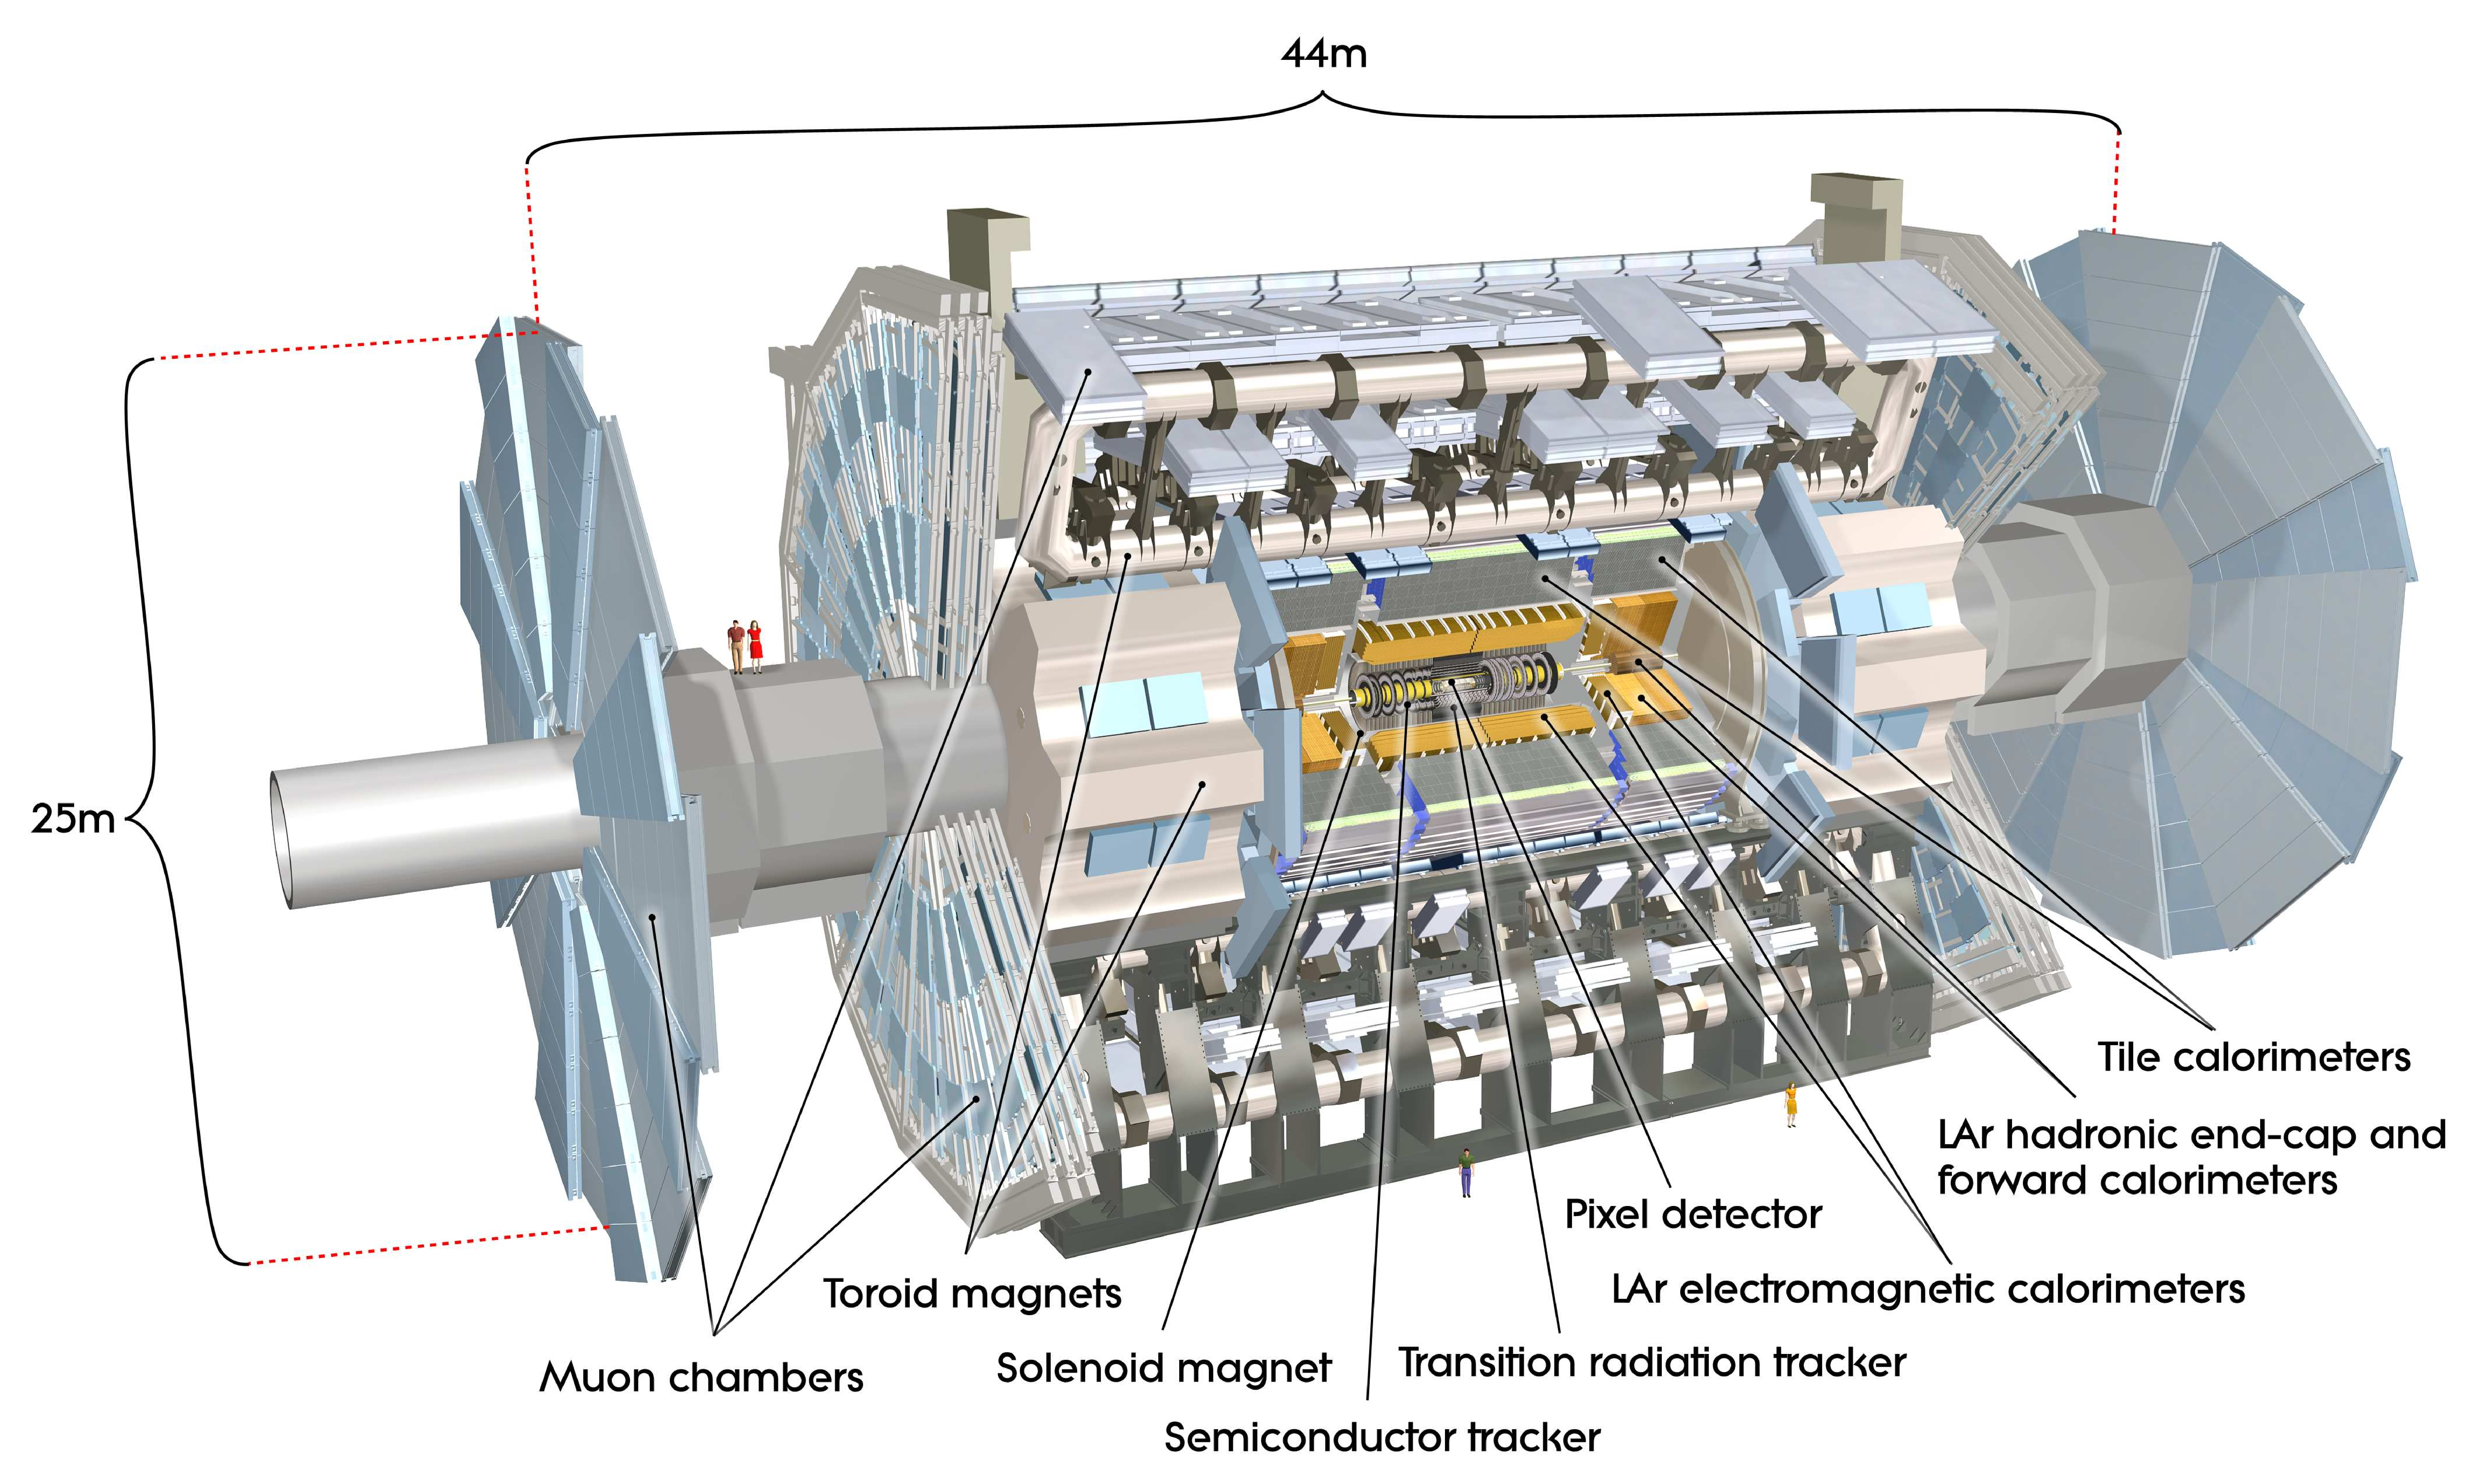
\includegraphics[width=\fullfig]{figures/atlas_overview.pdf}
\caption{A cut-away schematic of the layout of the \ac{ATLAS} detector. Each of the major subsystems is indicated.}
\label{fig:atlas_overview}
\end{figure}

\begin{figure}[hbtp]
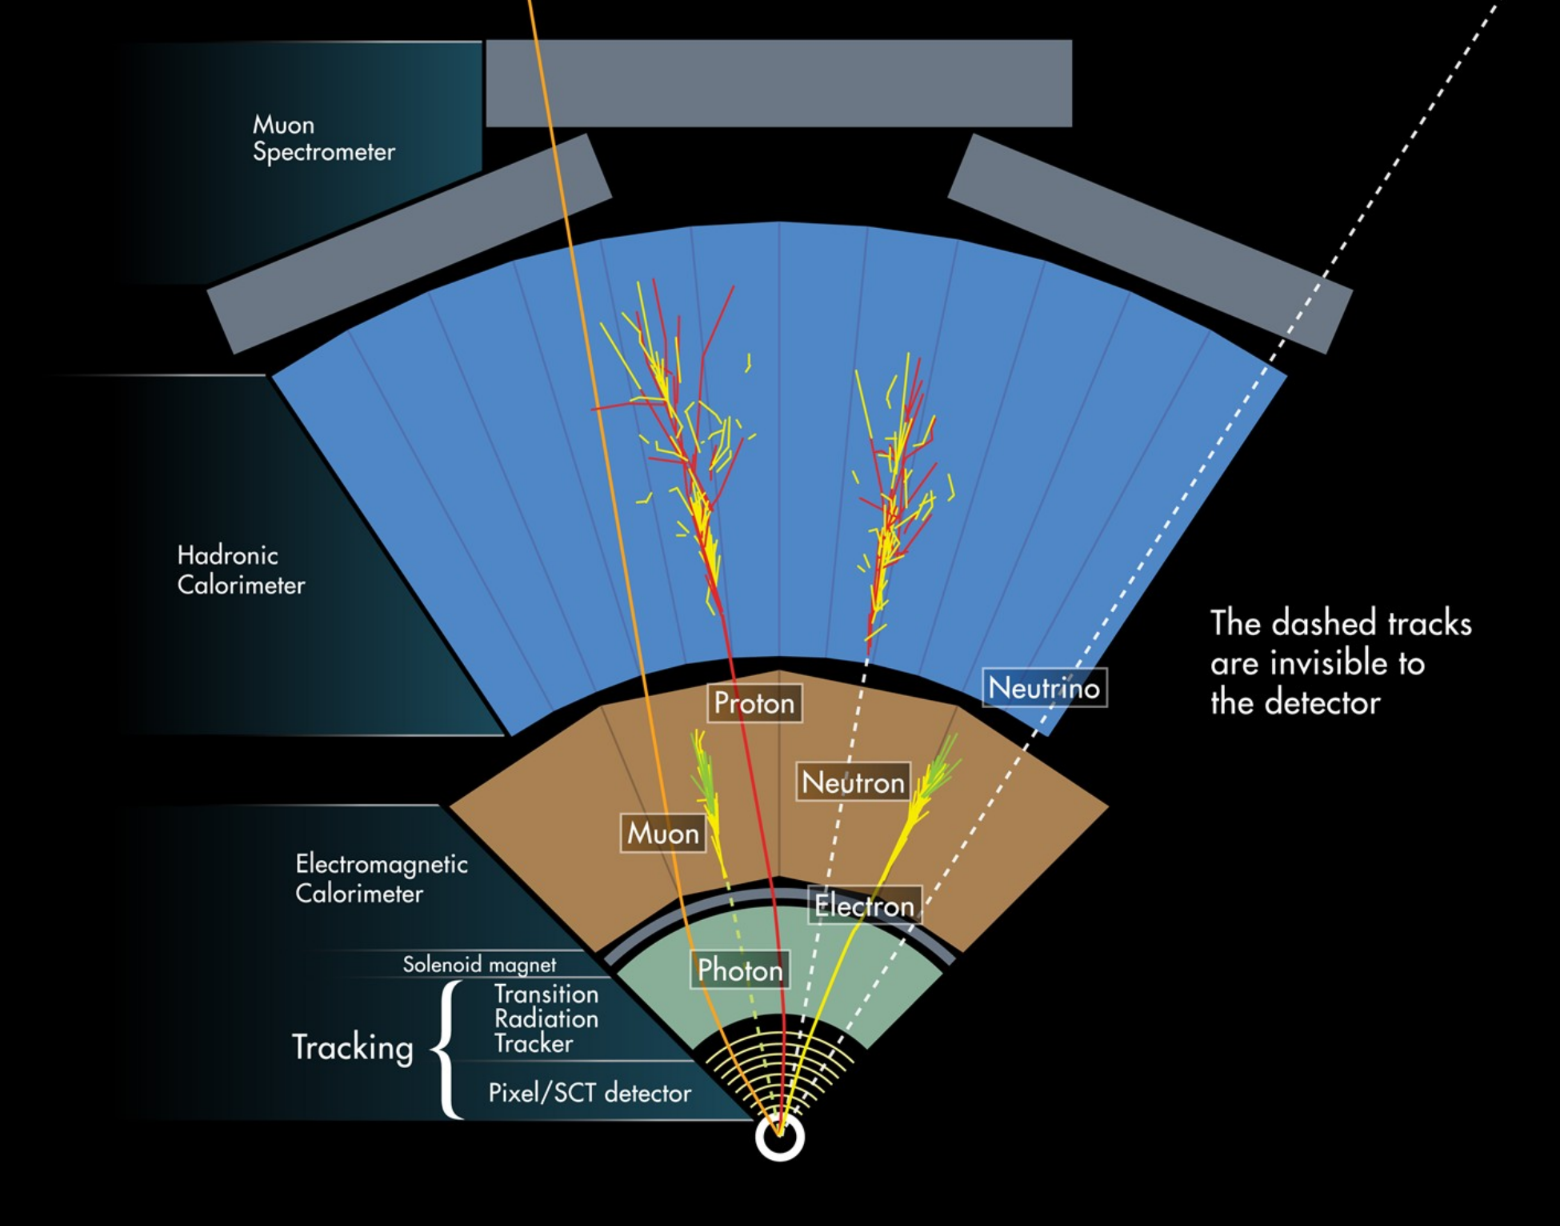
\includegraphics[width=\fullfig]{figures/particle_interactions.png}
\caption{A cross-sectional slice of the \ac{ATLAS} experiment which illustrates how the various \ac{SM} particles interact with the detector systems.}
\label{fig:particle_interactions}
\end{figure}

\begin{table}
\centering
\begin{tabular}{llcc}
  \hline
  Detector Component & Required Resolution & \multicolumn{2}{c}{$|\eta|$ Coverage} \\
                     &                     & Measurement & Trigger \\
  \hline
  Tracking & $\sigma_{\pt}/\pt = 0.05\% \pt + 1\%$ & $2.5$ & - \\
  EM Calorimetry & $\sigma_{E}/E = 10\%/\sqrt{E} + 0.7\%$ & $3.2$ & $2.5$ \\
  Hadronic Calorimetry & & \\
  \quad Barrel and Endcap & $\sigma_{E}/E = 50\%/\sqrt{E} + 3\%$ & $3.2$ & $3.2$ \\
  \quad Forward & $\sigma_{E}/E = 100\%/\sqrt{E} + 10\%$ & $3.1 - 4.9$ & $3.1 - 4.9$ \\
  Muon Spectrometer & $\sigma_{\pt}/\pt = 10\%$ at $p_T = 1\ \TeV$ & $2.7$ & $2.4$ \\
  \hline
\end{tabular}
\caption{The performance goals for each of the subsystems of the \ac{ATLAS} detector. The $|\eta|$ coverage specifies the range where the subsystem needs to be able to provide measurements with the specified resolution. The resolutions include a \pt or E dependence that is added in quadrature with a \pt/E independent piece.}
\label{tab:performance_goals}
\end{table}

Incorporating these various pieces into a single detector is a significant technical challenge.
The resulting detector has a diameter of 22 m, is 46 m long, and weighs 7,000 tons; it is the largest volume particle detector ever constructed.
The various detector elements need to be constructed and assembled with precisions as low as micrometers.
These systems all need to function well even after exposure to the significant radiation dose from the collisions.
Designing, constructing, and installing the detector took the combined effort of more than 3000 scientists from 38 countries over almost two decades.


\section{Coordinate System}

The coordinate system defined for the \ac{ATLAS} detector is used throughout all of the sections of this thesis.
The choice of coordinate system reflects the cylindrical symmetry of the \ac{ATLAS} detector, and is oriented by the direction of the beamline which defines the $z$-direction.
The positive $z$ side of the detector is commonly referred to as the $A$-side, and the negative $z$ side is referred to as the $C$-side.
The $x-y$ plane is then the plane transverse to the beam direction, with the $x$ direction defined as pointing from the interaction point to the center of the \ac{LHC} ring and the $y$ direction defined as pointing upwards.
The nominal interaction point is the origin of this system.

It is more convenient in practice to use a cylindrical coordinate system.
The angle from the $z$-axis is $\theta$.
The azimuthal angle uses the usual definition, with $\phi$ running around the $z$-axis and $\phi = 0$ corresponding to the $x$-axis.
Many aspects of the detector are independent of the this coordinate to first order.
The remaining direction is typically specified using rapidity or pseudorapidity, where rapidity is defined as

\begin{equation}\label{eq:rapidity}
y = \frac{1}{2} \ln \frac{E + p_z}{E - p_z}
\end{equation}

\noindent Rapidity is particularly useful to indicate the component along the $z$ direction because differences in rapidity are invariant to boosts along the $z$-direction.
A similar quantity which depends only the $\theta$ is pseudorapidity, 

\begin{equation}\label{eq:pseudorapidity}
\eta = - \ln \tan \frac{\theta}{2}
\end{equation}

\noindent which is the same as rapidity when the particle is massless and in the limit where the energy is much larger than the particle's mass.
It is often useful to refer to differences in solid angle using the pseudorapdity and the azimuthal angle:

\begin{equation}\label{eq:deltar}
\Delta R = \sqrt{\Delta \phi^2 + \Delta \eta^2}
\end{equation}


The pseudorapdity is also invariant to boosts along the $z$-axis for high momentum particles, and is preferable to rapidity because it does not depend on the specific choice of particle.
Pseudorapidity is also preferable to $\theta$ because of the afformentioned boost-invariance and also because particle production is roughly uniform in equal-width intervals of $\eta$ up to about $\eta = 5.0$. 
A particle travelling along the beampipe has $\eta = \inf$ and a particle travelling perpendicular to the beampipe has $\eta = 0$.
The extent of the tracker, $|\eta| < 2.5$, corresponds to approximately $0.05 \pi < \theta [\mathrm{rad}] < 0.95 \pi$ and the extent of the calorimeters, $|\eta| < 4.9$ corresponds to approximately $0.005 \pi < \theta [\mathrm{rad}] < 0.995 \pi$.
Many detector components are broken into multiple subsystems to provide coverage at greater $|\eta|$.
The lower $|\eta|$ region is referred to as the barrel, typically with $|\eta| \lesssim 2$, and the greater $|\eta|$ region is often referred to as the endcap.

The initial energy and momentum of a proton-proton collision along the $z$ direction is unknown in hadron colliders because different energies and momentums can be carried by the partons.
Along the transverse plane, however, the vector sum of momentum will be zero.
For this reason, many physical quantities are quantified in terms of their projection onto the transverse plan, such as \pt or $E_T$.
In addition, \pt alone determines the amount of curvature in the magnetic field, and can be measured independently by measuring the curvature of a particle's propagation.


\section{Magnetic Field}
\label{sec:magnetic_field}

The magnet system used in \ac{ATLAS} is designed to provide a substantial magnetic field in the two regions where the trajectory of particles is measured, the inner detector and the muon spectrometer.
The magnetic field provides a curvature to the trajectory of charged particles and allows the precision tracking measurements to make high resolutions measurements of \pt.
To provide a magnetic field in these regions, \ac{ATLAS} uses a hybrid system with four separate, superconducting magnets.
A single solenoid provides a 2 T axial magnetic field for the inner detector, while a barrel toroid and two endcap toroids produce a magnetic field of 0.5 and 1 T, respectively, for the muon detectors.
This geometry is illustrated in Figure~\ref{fig:magnets_overview}, and the parameters of the three magnet systems are summarized in Table~\ref{tab:magnet_parameters}.

\begin{figure}[hbtp]
\centering
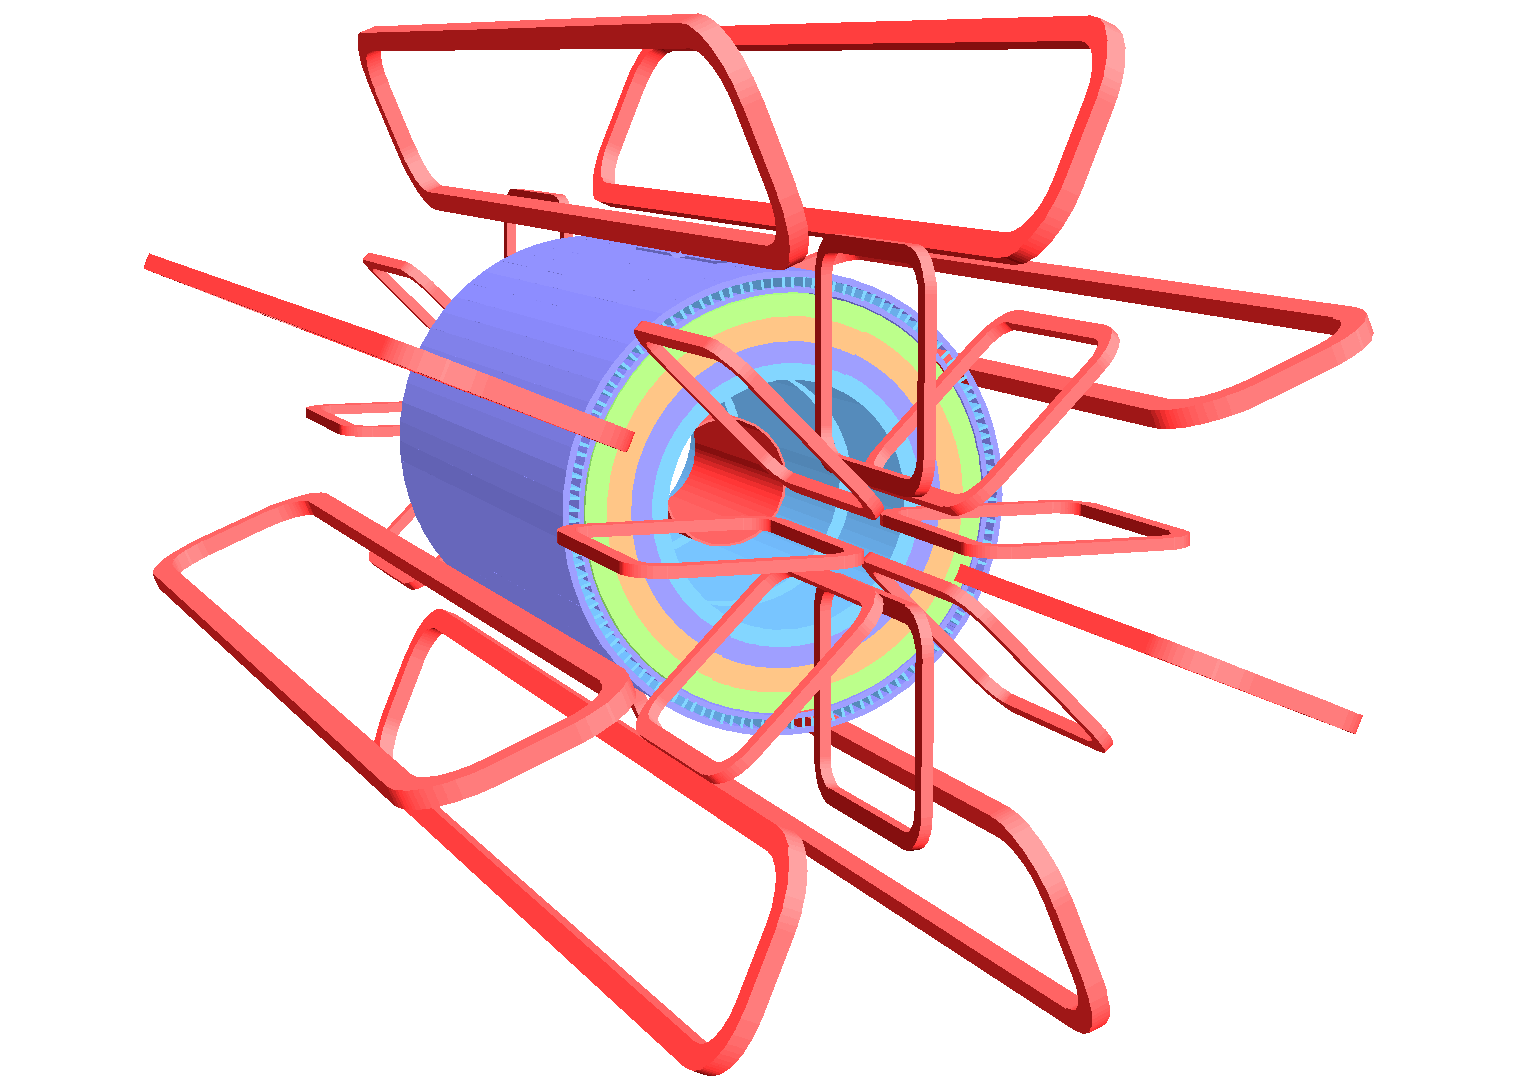
\includegraphics[width=\fullfig]{figures/magnets_overview.pdf}
\caption{The layout of the four superconducting magnets in the \ac{ATLAS} detector.}
\label{fig:magnets_overview}
\end{figure}

\begin{table}
\centering
\begin{tabular}{lcccc}
\hline
Parameter & Unit & Solenoid & Barrel Toroid & Endcap Toroids \\
\hline
Inner Diamater & m & 2.4 & 9.4 & 1.7 \\
Outer Diamater & m & 2.6 & 20.1 & 10.7 \\
Axial Length & m & 5.3 & 25.3 & 5.0 \\
Weight & tons & 5.7 & 830 & 239 \\
Conductor Size & mm\tsup{2} & 30$\times$4.25 & 57$\times$12 & 41$\times$4.25 \\
Peak Field & T & 2.6 & 3.9 & 4.1\\
Heat Load & W & 130 & 990 & 330 \\
Current & kA & 7.7 & 20.5 & 20.0 \\
Stored Energy & MJ & 38 & 1080 & 206 \\
\hline
\end{tabular}
\label{tab:magnet_parameters}
\end{table}

The central solenoid uses a single-layer coil with a current of 7.730 kA to generate the 2 T axial field at the center of the magnet. 
The single-layer coil design enables a minimal amount of material to be used in the solenoid's construction, which is important because the solenoid is placed between the inner detector and the calorimeters.
At normal incidence the magnet has only 0.66 radiation lengths worth of material, where one radiation length is the mean distance over which a high-energy electron loses all but $1/e$ of its energy through material interactions~\cite{pdg}.
The coil is made of a high-strength aluminum stabilized NbTi superconductor which was optimized to achieve a high field with minimal thickness.
The axial magnetic field produced by the solenoid bends charged particles in the $\phi$ direction.

The barrel toroid consists of eight coils which generate a 0.5 T magnetic field in the cylindrical region around the calorimeters with an approximately 20 kA current.
The coils are separated only by air to reduce the scattering of muons as they propogate through the region.
The coils are made of an aluminum stabilized NbTiCu superconductor and each is separately housed in a vacuum and cold chamber.
This magnetic configuration produces a field in the $\phi$ and so curves muons traversing the volume primarily in the $\eta$ direction.

The endcap toroids follow a similar design to the barrel toroid, with eight separate NbTiCu coils, but in this case all eight are housed within a single cold mass.
This extra structure is necessary to withstand the Lorentz forces exerted by the magnets. 
These magnets are rotated 22.5\% relative to the barrel toroid to provide a uniform field in the transition between the two systems. 
The endcap toroids also produce a field in the $\phi$ direction and curve muons primarily in the $\eta$ direction.

% ----------------------------------------

\section{Inner Detector}
\label{sec:inner_detector}

The \ac{ATLAS} inner detector provides excellent momentum resolution as well as accurate primary and secondary vertex measurements through robust pattern recognition that identifies tracks left by charged particles. 
These tracks fulfill a number of important roles in the \ac{ATLAS} measurement system: they measure the momentum of charged particles inluding electrons and muons, they can identify electrons or photon conversions, they assign various particles and jets to different vertices, and they provide a correction to \met measurements from low energy particles. 
The system has to be accurate enough to separate tracks from dozens of verticies and to resolve each vertex individually, as well as accurate enough to measure the \pt of very high momentum tracks which curve very little even in the large magnetic field.
This is accomplished by several independent layers of tracking systems.
Closest to the interaction point is the very high granulity Pixel detector, which is followed by the \ac{SCT} layers.
These subdetectors both use discrete space-points to reconstruct track patterns.
The final layer, the \ac{TRT}, uses many layers of straw tube elements interleaved with transition radiation material to provide continuous tracking.
The arrangement of these subdetectors is shown in Figure~\ref{fig:id_overview}.
To provide the desired hermetic coverage, the subdetectors are divided into barrel and endcap geometries.
Figure~\ref{fig:id_detail_schematic} shows the layout of the subdetectors in more detail, and illustrates how tracks at various pseudorapidities can traverse the subdetectors; tracks with $\eta > 1.1$ begin to traverse the endcap subdetectors rather than those in the barrel, and tracks with $\eta > 1.7$ use primarily endcap elements. 
The \ac{IBL} was not present during the original commisioning of the inner detector and is not shown in this figure.

\begin{figure}[hbtp]
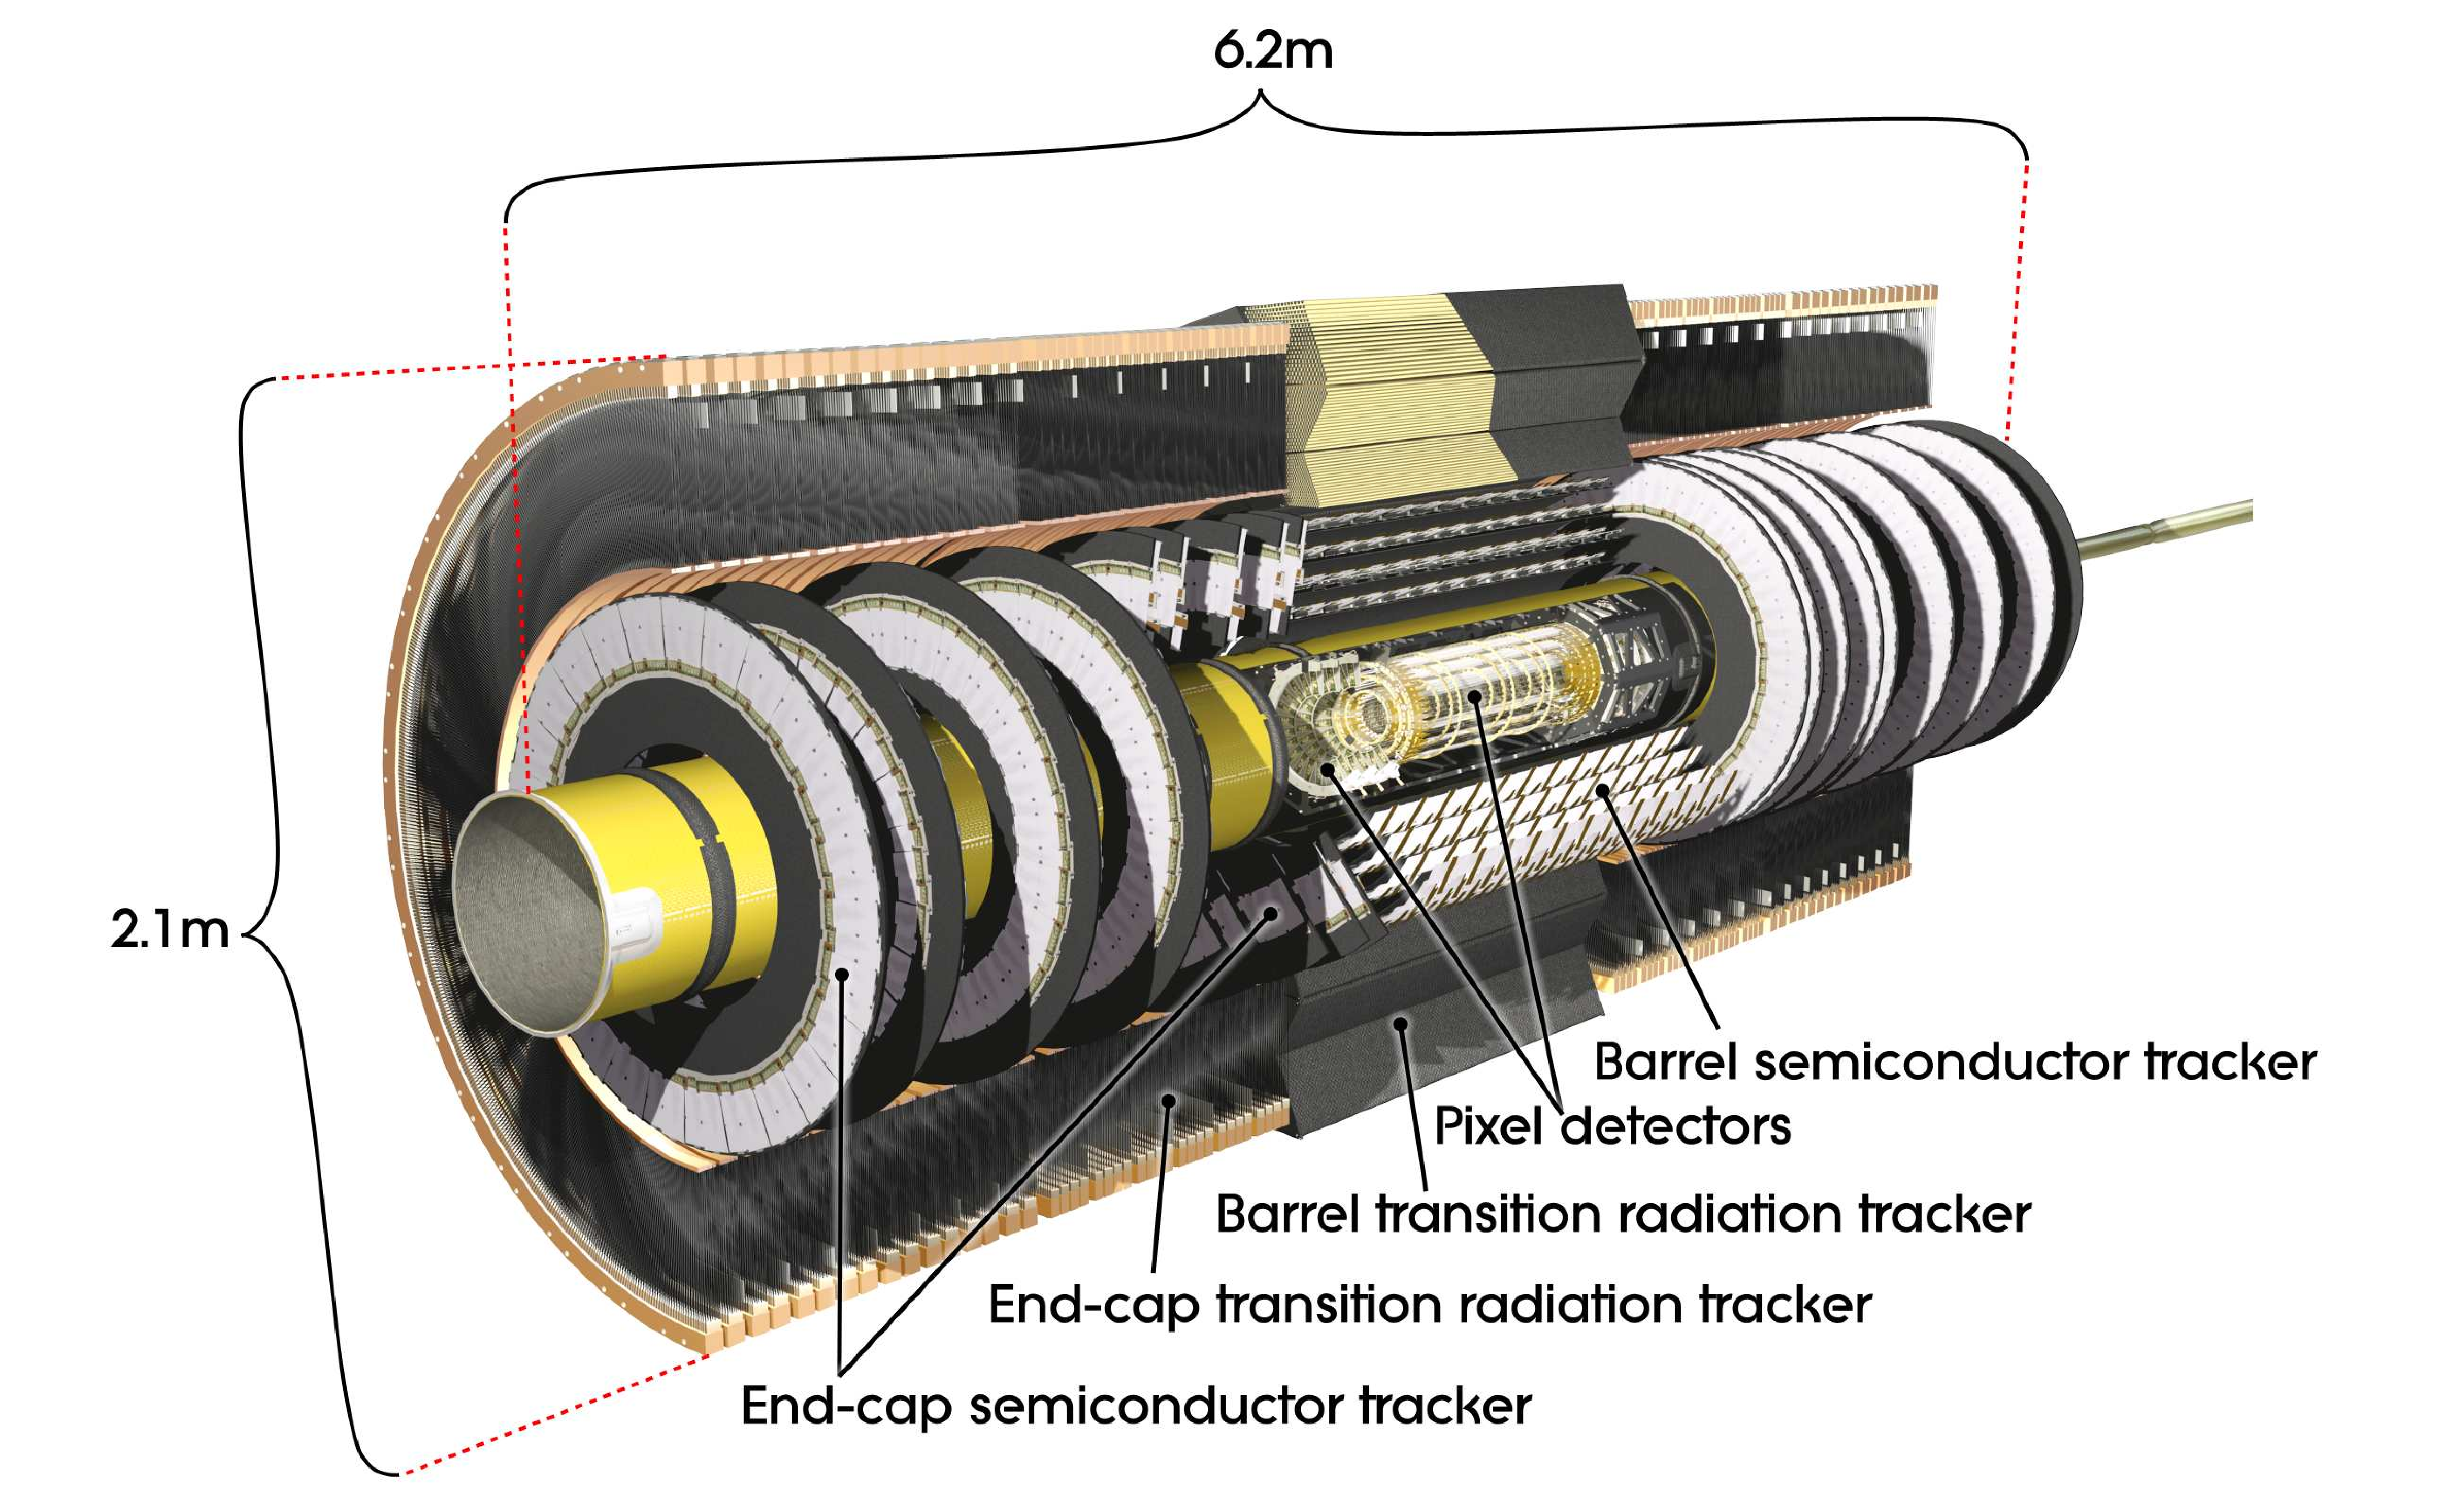
\includegraphics[width=\fullfig]{figures/id_overview.pdf}
\caption{The arrangement of the subdetectors of the \ac{ATLAS} inner detector. Each of the subdetectors is labelled in the cut-away view of the system.}
\label{fig:id_overview}
\end{figure}

\begin{figure}[hbtp]
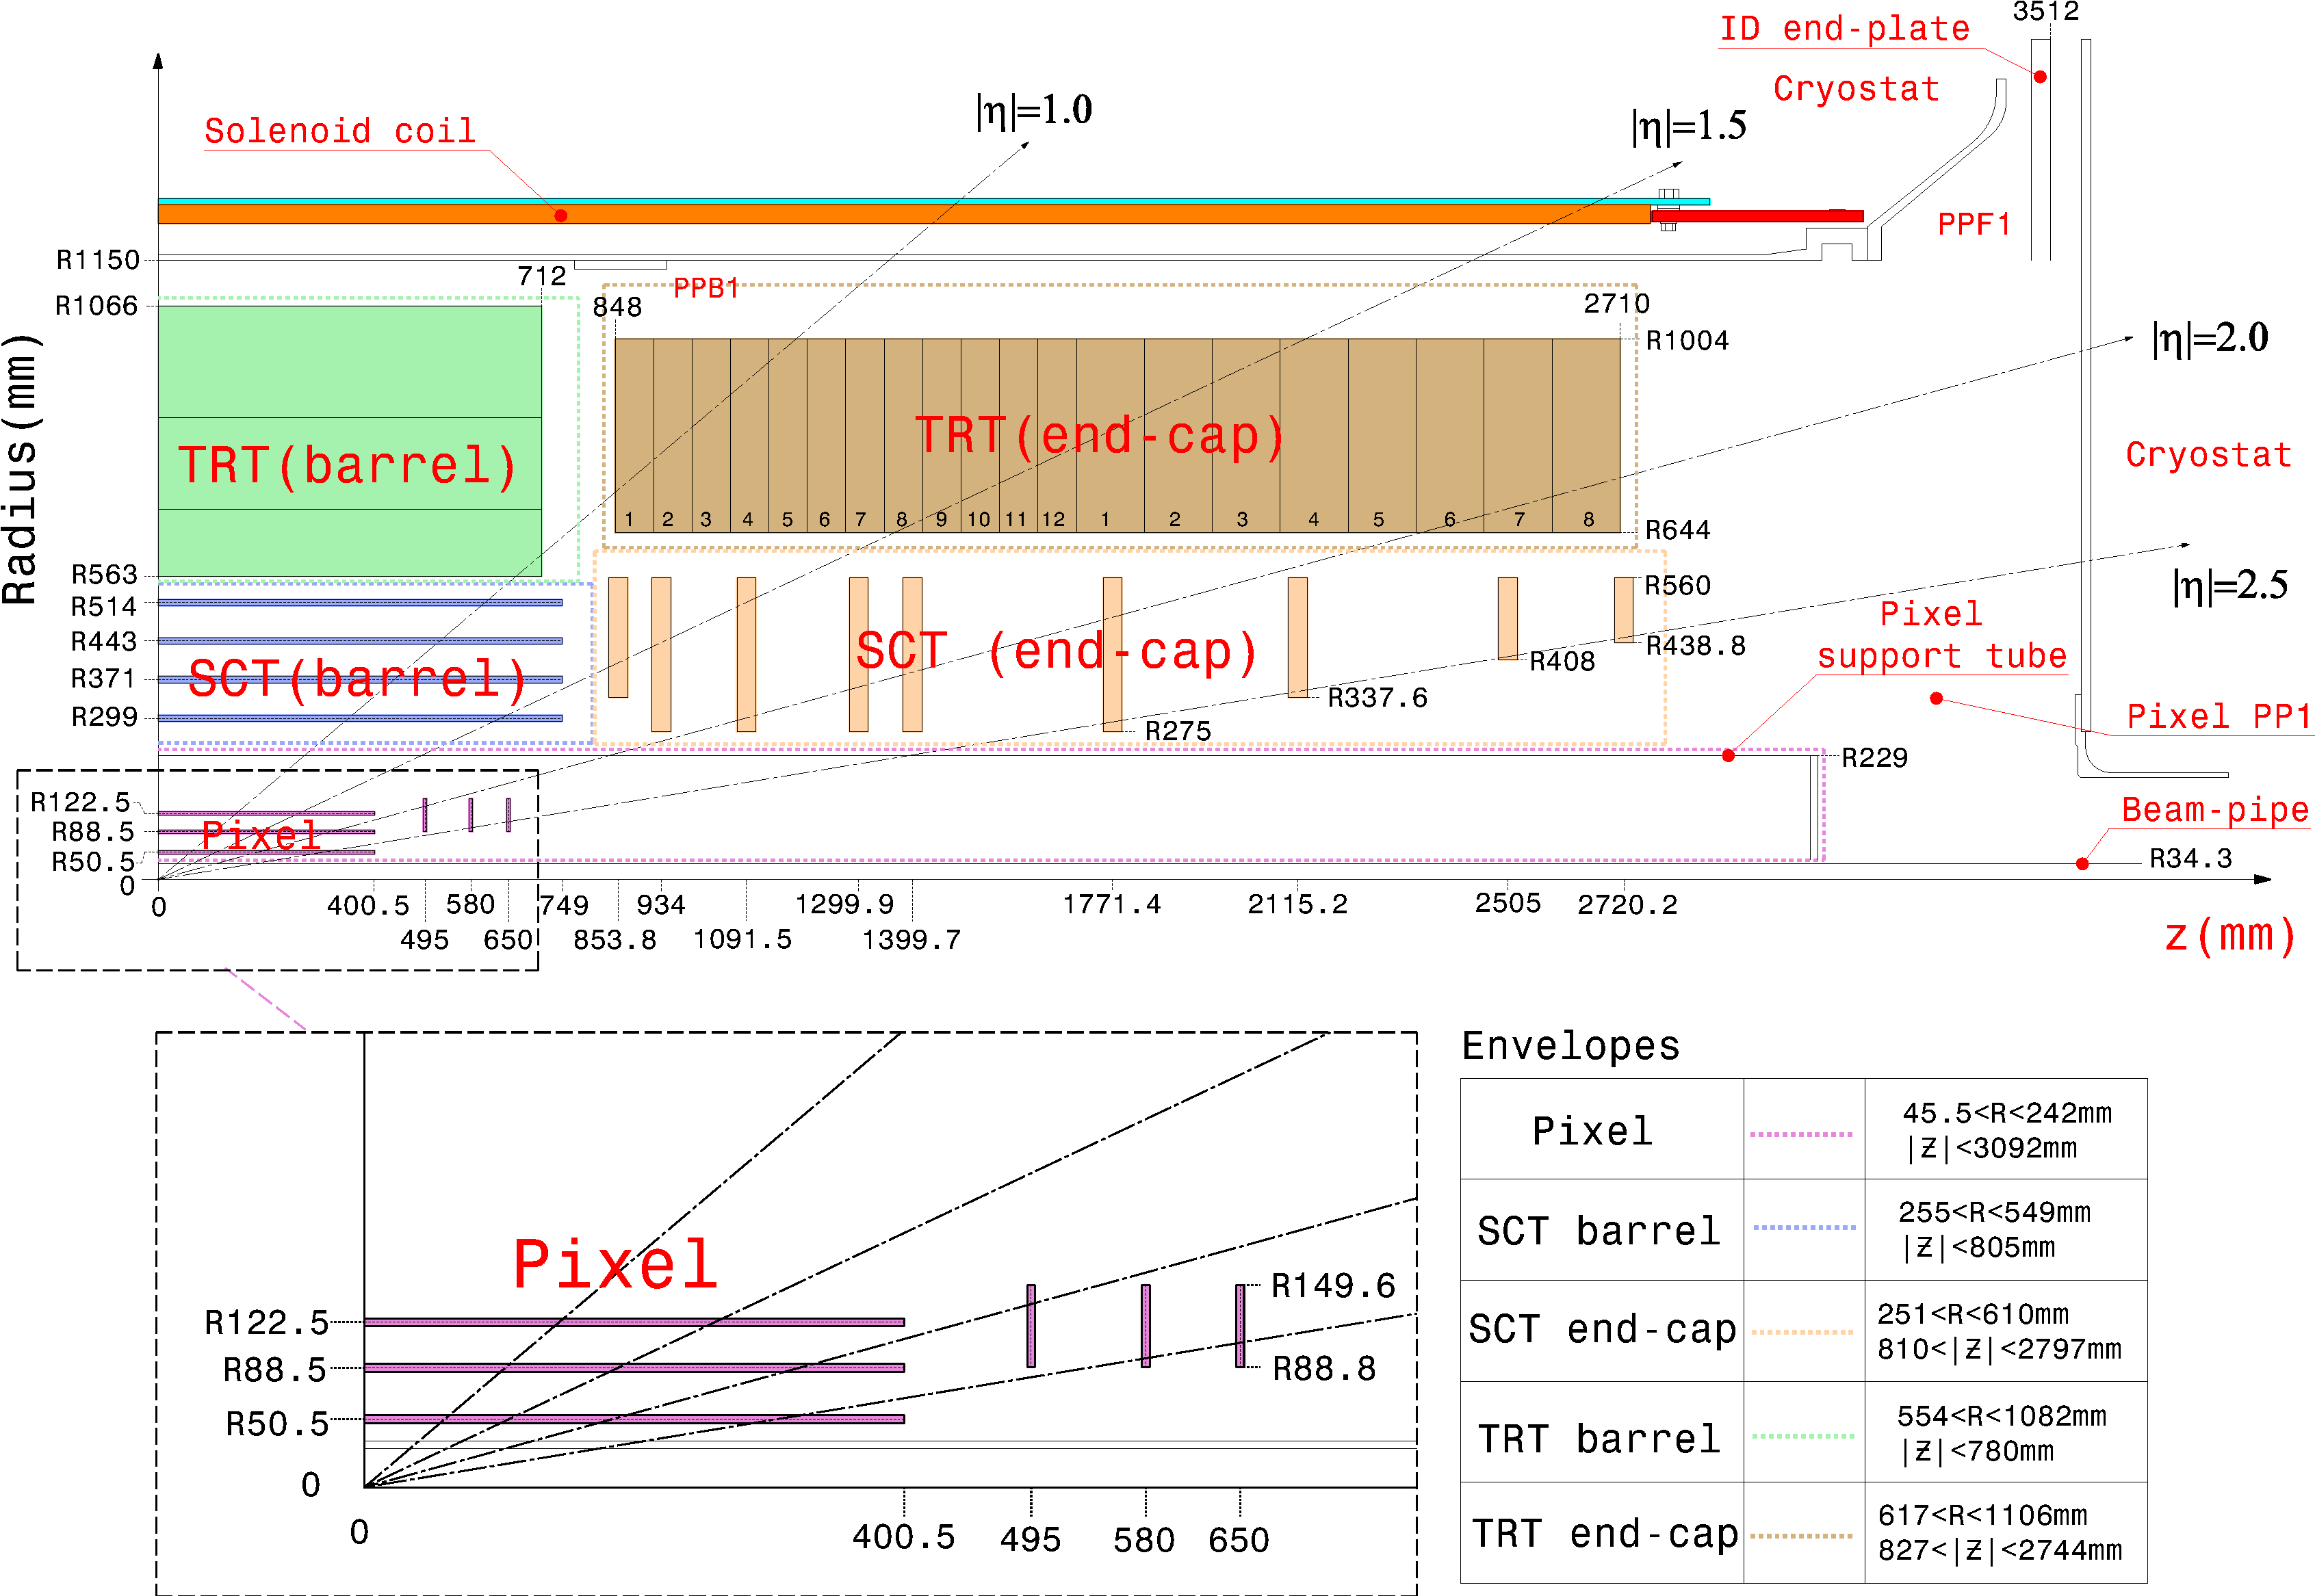
\includegraphics[width=\fullfig]{figures/id_detail_schematic.pdf}
\caption{A quarter section of the \ac{ATLAS} inner detector which shows the layout of each of the subdetectors in detail. The lower panel shows an enlarged view of the pixel detector. Example trajectories for a particle with $\eta = 1.0, 1.5, 2.0, 2.5$ are shown. The \ac{IBL}, which was added after the original detector commisioning, is not shown.}
\label{fig:id_detail_schematic}
\end{figure}

Figure ~\ref{fig:id_slice} shows a computer generated three-dimensional view of the inner detector along the beam axis, which emphasizes the straw tube structure of the \ac{TRT} as well as the overlapping geometry of the \ac{SCT}.
This figure also includes the \ac{IBL}, which was added during the long shutdown and provides an additional measurement layer in the Pixel detector as of the beginning of Run 2. 
Figure ~\ref{fig:id_slice_long} shows an alternative computer generated three-dimensional view transverse to the beam axis which emphasizes the endcap structures of the \ac{SCT} and \ac{TRT}. 

\begin{figure}[hbtp]
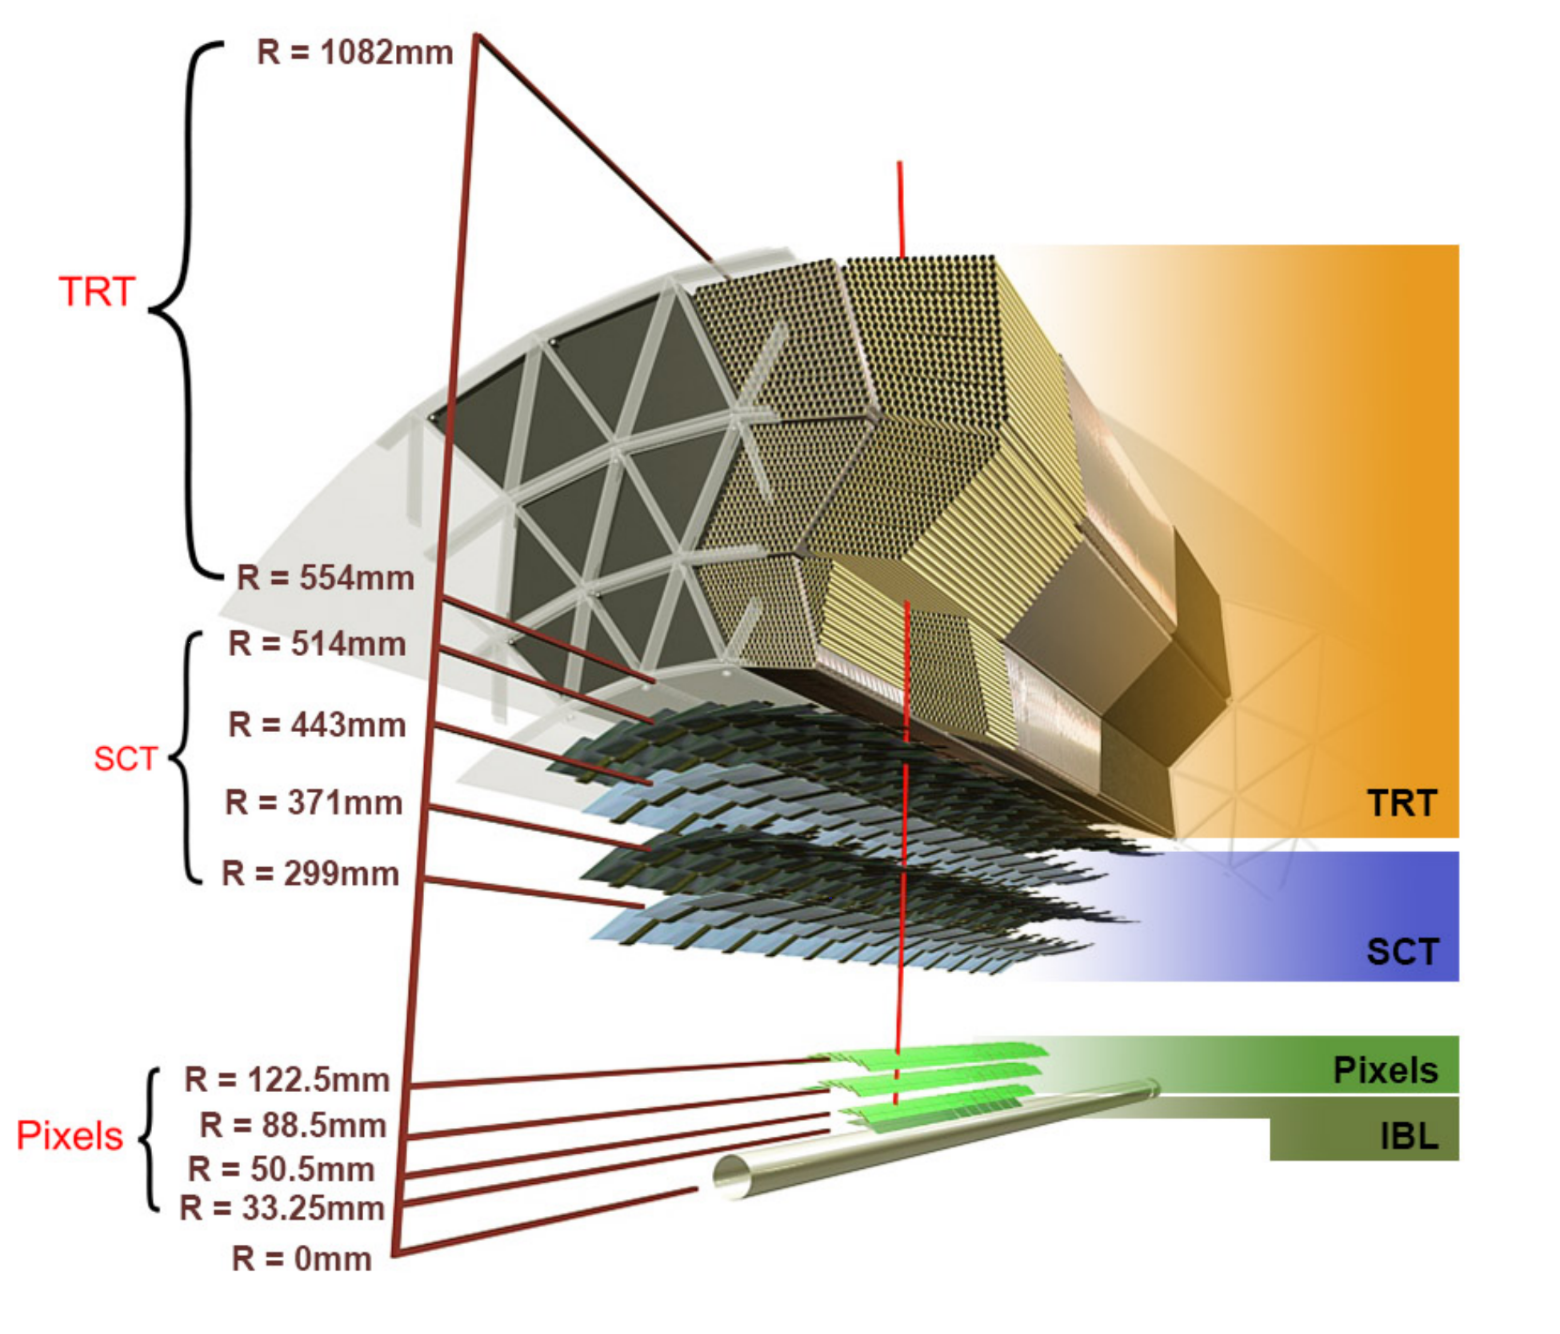
\includegraphics[width=\fullfig]{figures/id_slice.png}
\caption{A computer generated three-dimensional view of the inner detector along the line of the beam axis. The subdetectors and their positions are labelled.}
\label{fig:id_slice}
\end{figure}


\begin{figure}[hbtp]
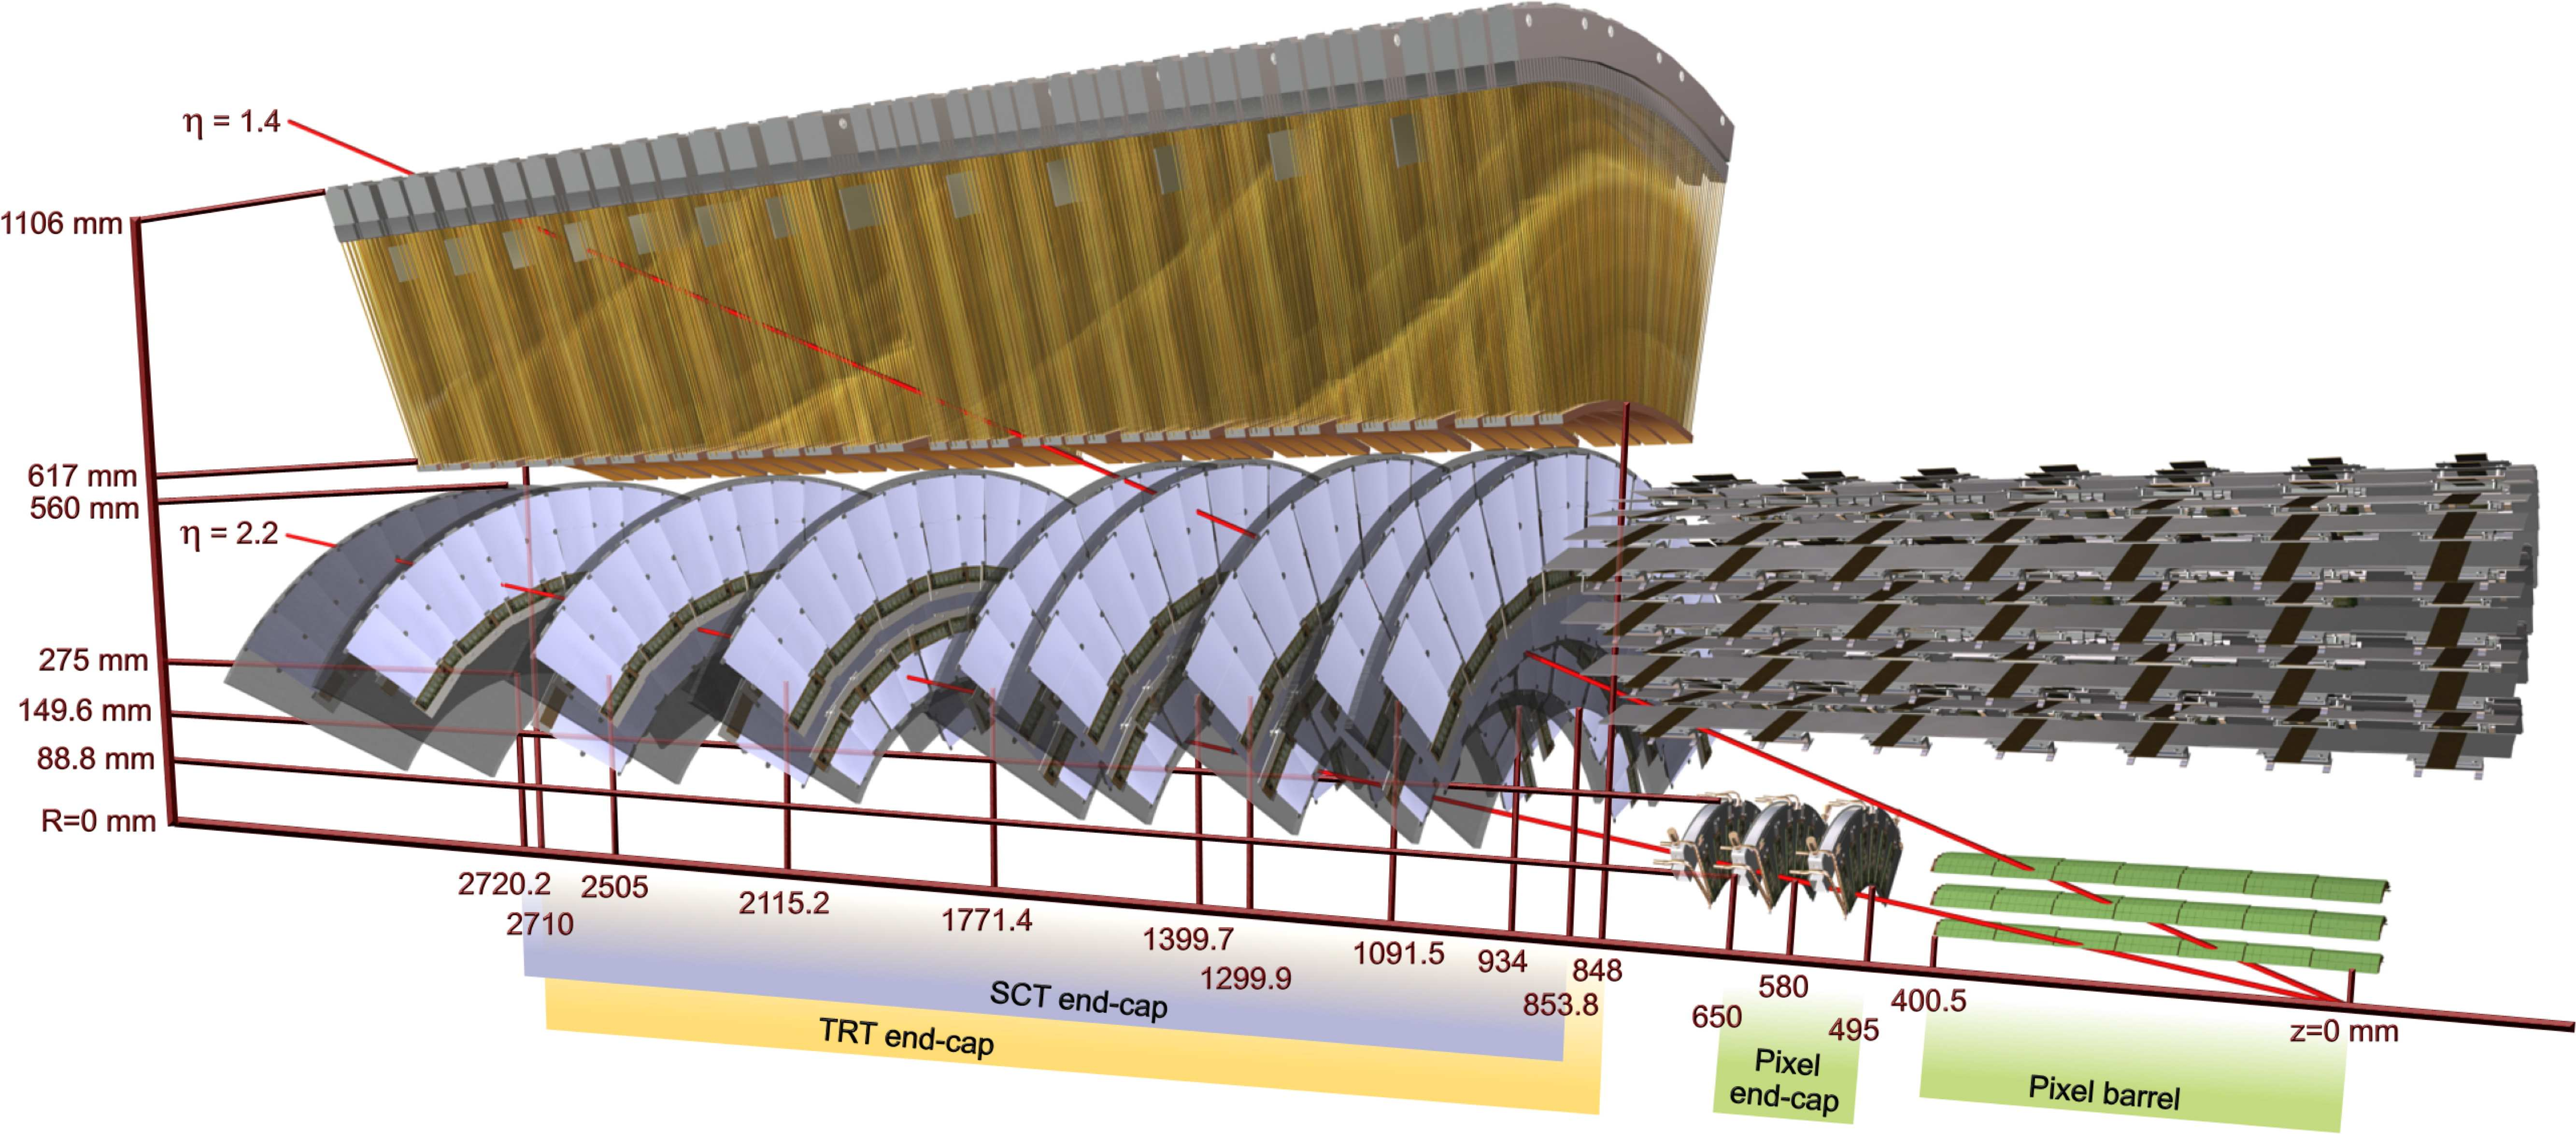
\includegraphics[width=\fullfig]{figures/id_slice_long.pdf}
\caption{An alternative computer generated three-dimensional view of the inner detector transverse to the beam axis. The subdetectors and their positions are labelled.}
\label{fig:id_slice_long}
\end{figure}

As the closest system to the interaction point, it is crucial for the inner detector to use as little material as possible to avoid scattering of charged particles or photon conversions before they reach the remaining subdetectors.
The various components, including the readout electronics, cooling infrastructure, gas volumes, and support structures,  were designed to use as little material as possible. 
Even with these optimizations, the combination of stringent performance requirements and the harsh radiation environment in the inner detector requires a significant amount of material.
This material causes many electrons to lose most of their energy before reaching the electromagnetic calorimeter and approximately 40\% of photons convert into an electron-positron pair while traversing the inner detector.
Figure~\ref{fig:id_material} shows the integrated radiation lengths traversed by a straight track in the inner detector as a function of $\eta$, grouped by subdetector.
There is a large increase in the amount of material for support structures around $|\eta| = 1.7$, where the inner detector transitions from barrel to endcap.


\begin{figure}
\centering
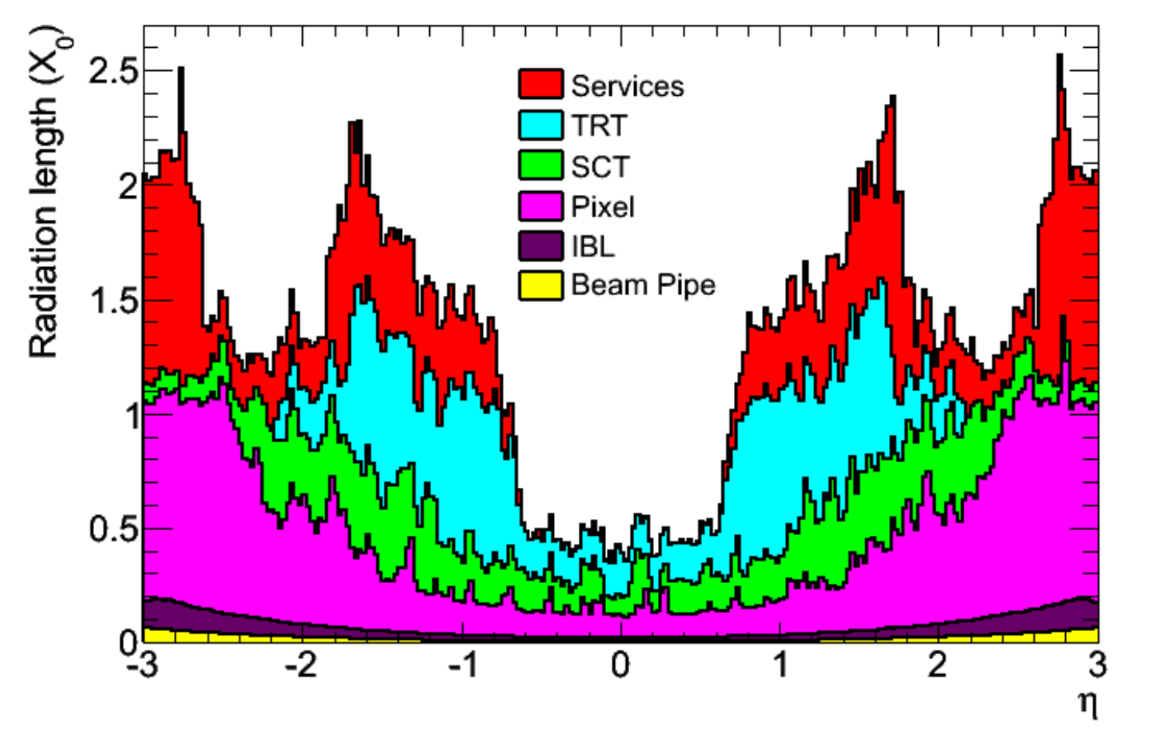
\includegraphics[width=\fullfig]{figures/id_material_subdetector.png}
\caption{The integrated radiation lengths traversed by a straight track at the exit of the ID envelope, including the services and thermal enclosures. The distribution is shown as a function of $|\eta|$ and averaged over $\phi$. The breakdown indicates the contributions of individual sub-detectors, including services in their active volume.}
\label{fig:id_material}
\end{figure}

The inner detector is designed to work as a cohesive unit to provide complete tracking information for charged particulars, and the subdetectors are complementary.
Table~\ref{tab:id_parameters} summarizes the parameters of each of the subdetectors as well as the parameters of the combined inner detector. 
Table ~\ref{tab:id_performance} summarizes the expected performance that can be acheived by the inner detector as a whole.

\begin{table}[h]
\begin{tabular}{lcccc}
\hline
Parameter & Inner Detector & Pixel & \ac{SCT} & \ac{TRT} \\
\hline
Inner Radius & 3.1 cm & 3.1 cm & 30 cm & 56 cm \\
$|\eta|$ Coverage & - & 2.5 & 2.5 & 2.0 \\
Cell Width & - & 50 \um & 80 \um & 4 mm \\
Cell Length & - & 400 \um & 12 cm & 70 cm \\
Material at $|\eta| = 0.0$ & 0.3 $X/X_0$ & & & \\
Material at $|\eta| = 1.7$ & 1.2 $X/X_0$ & & & \\
Material at $|\eta| = 2.5$ & 0.5 $X/X_0$ & & & \\
\hline
Number of Hits & 48 & 4 & 8 & 36 \\
Channels & 99 M & 92 M & 6.3 M & 350 k \\
\hline
\end{tabular}
\caption{A summary of the parameters of the inner detector and each of the subdetectors~\cite{atlas_experiment}.}
\label{fig:id_parameters}
\end{table}

\begin{table}[h]
\begin{tabular}{lll}
\hline
Parameter & Particle & Value \\
\hline
Reconstruction Efficiency & Muon, $\pt = 1\ \GeV$ & 96.8\% \\
  & Pion, $\pt = 1\ \GeV$ & 84.0\% \\
  & Electron, $\pt = 5\ \GeV$ & 90.0\% \\
Momentum Resolution & $\pt = 1\ \GeV$, $|\eta| \approx 0$ & 1.3\% \\
  & $\pt = 1\ \GeV$, $|\eta| \approx 2.5$ & 2.0\% \\
  & $\pt = 100\ \GeV$, $|\eta| \approx 0$ & 3.8\% \\
  & $\pt = 100\ \GeV$, $|\eta| \approx 2.5$ & 11\% \\
Transverse \acs{IP} Resolution & $\pt = 1\ \GeV$, $|\eta| \approx 0$ & 75 \um\% \\
  & $\pt = 1\ \GeV$, $|\eta| \approx 2.5$ & 200 \um \\
  & $\pt = 1000\ \GeV$, $|\eta| \approx 0$ & 11 \um \\
  & $\pt = 1000\ \GeV$, $|\eta| \approx 2.5$ & 11 \um \\
Longitudinal \acs{IP} Resolution & $\pt = 1\ \GeV$, $|\eta| \approx 0$ & 150 \um\% \\
  & $\pt = 1\ \GeV$, $|\eta| \approx 2.5$ & 900 \um \\
  & $\pt = 1000\ \GeV$, $|\eta| \approx 0$ & 90 \um \\
  & $\pt = 1000\ \GeV$, $|\eta| \approx 2.5$ & 190 \um \\
\hline
\end{tabular}
\caption{A summary of the expected performance of the combined inner detector~\cite{gpd_lhc}. Included are the reconstruction effiencies for multiple particle types as well as the momentum and \ac{IP} resolution for various momenta.}
\label{fig:id_parameters}
\end{table}


\subsection{Pixel Detector}
\label{sec:pixel}
The Pixel detector is the closest detector to the interaction point and therefore is designed to provide extremely high granularity while simultaneously handling a very large dose of radiation from collisions.
It consists of four layers of silicon pixel modules, each of which provides a precision measurement on the trajectory of any charged particle.
In the barrel region, the four layers are located at radial distances of 31 mm, 51 mm, 89 mm, and 123 mm. 
The three outer layers also include endcap elements, illustrated in Figure~\ref{fig:id_detail_schematic}, which are located at 495 mm, 580 mm, and 650 mm away from the interaction point. 

The pixel sensor technology uses a p-n junction of n-type bulk that contains both p\tsup{+} and n\tsup{+} impurities.
This combination is crucial in maintaining performance after a significant radiation dose, as the n\tsup{+} implants allow the sensor to continue function after the n-type bulk has been converted to a p-type bulk by the accumulation of radiation.

The size of the pixels in the original three layers are 50 \um x 400 \um in the $r-\phi$ and $z$ directions, respectively.
Those pixels are bump-bonded to front-end readout chips, the FE-I3, which contains a total of 2880 pixels per chip. 
In the three original pixel layers, the chips are grouped into modules composed of 16 chips each with 46,080 pixels per module and a total size of 20 mm x 60 mm x 250 \um. 
The modules are further arranged into long rectangular structures that run parallel to the beamline called staves.
By tiling several staves with an offset of 20\textdegree, the stave geometry provides full azimuthal coverage in the barrel region while accomodating the readout and cable systems.
The endcap regions are instead arranged into petals and then into wheels. 
This arrangement can be seen in Figure~\ref{fig:pixel_overview} which shows a computer-generated, cut-away image of the outer three layers of the pixel detector.
Together these three layers contain 1744 modules between the barrel and two endcap sections.

\begin{figure}[hbtp]
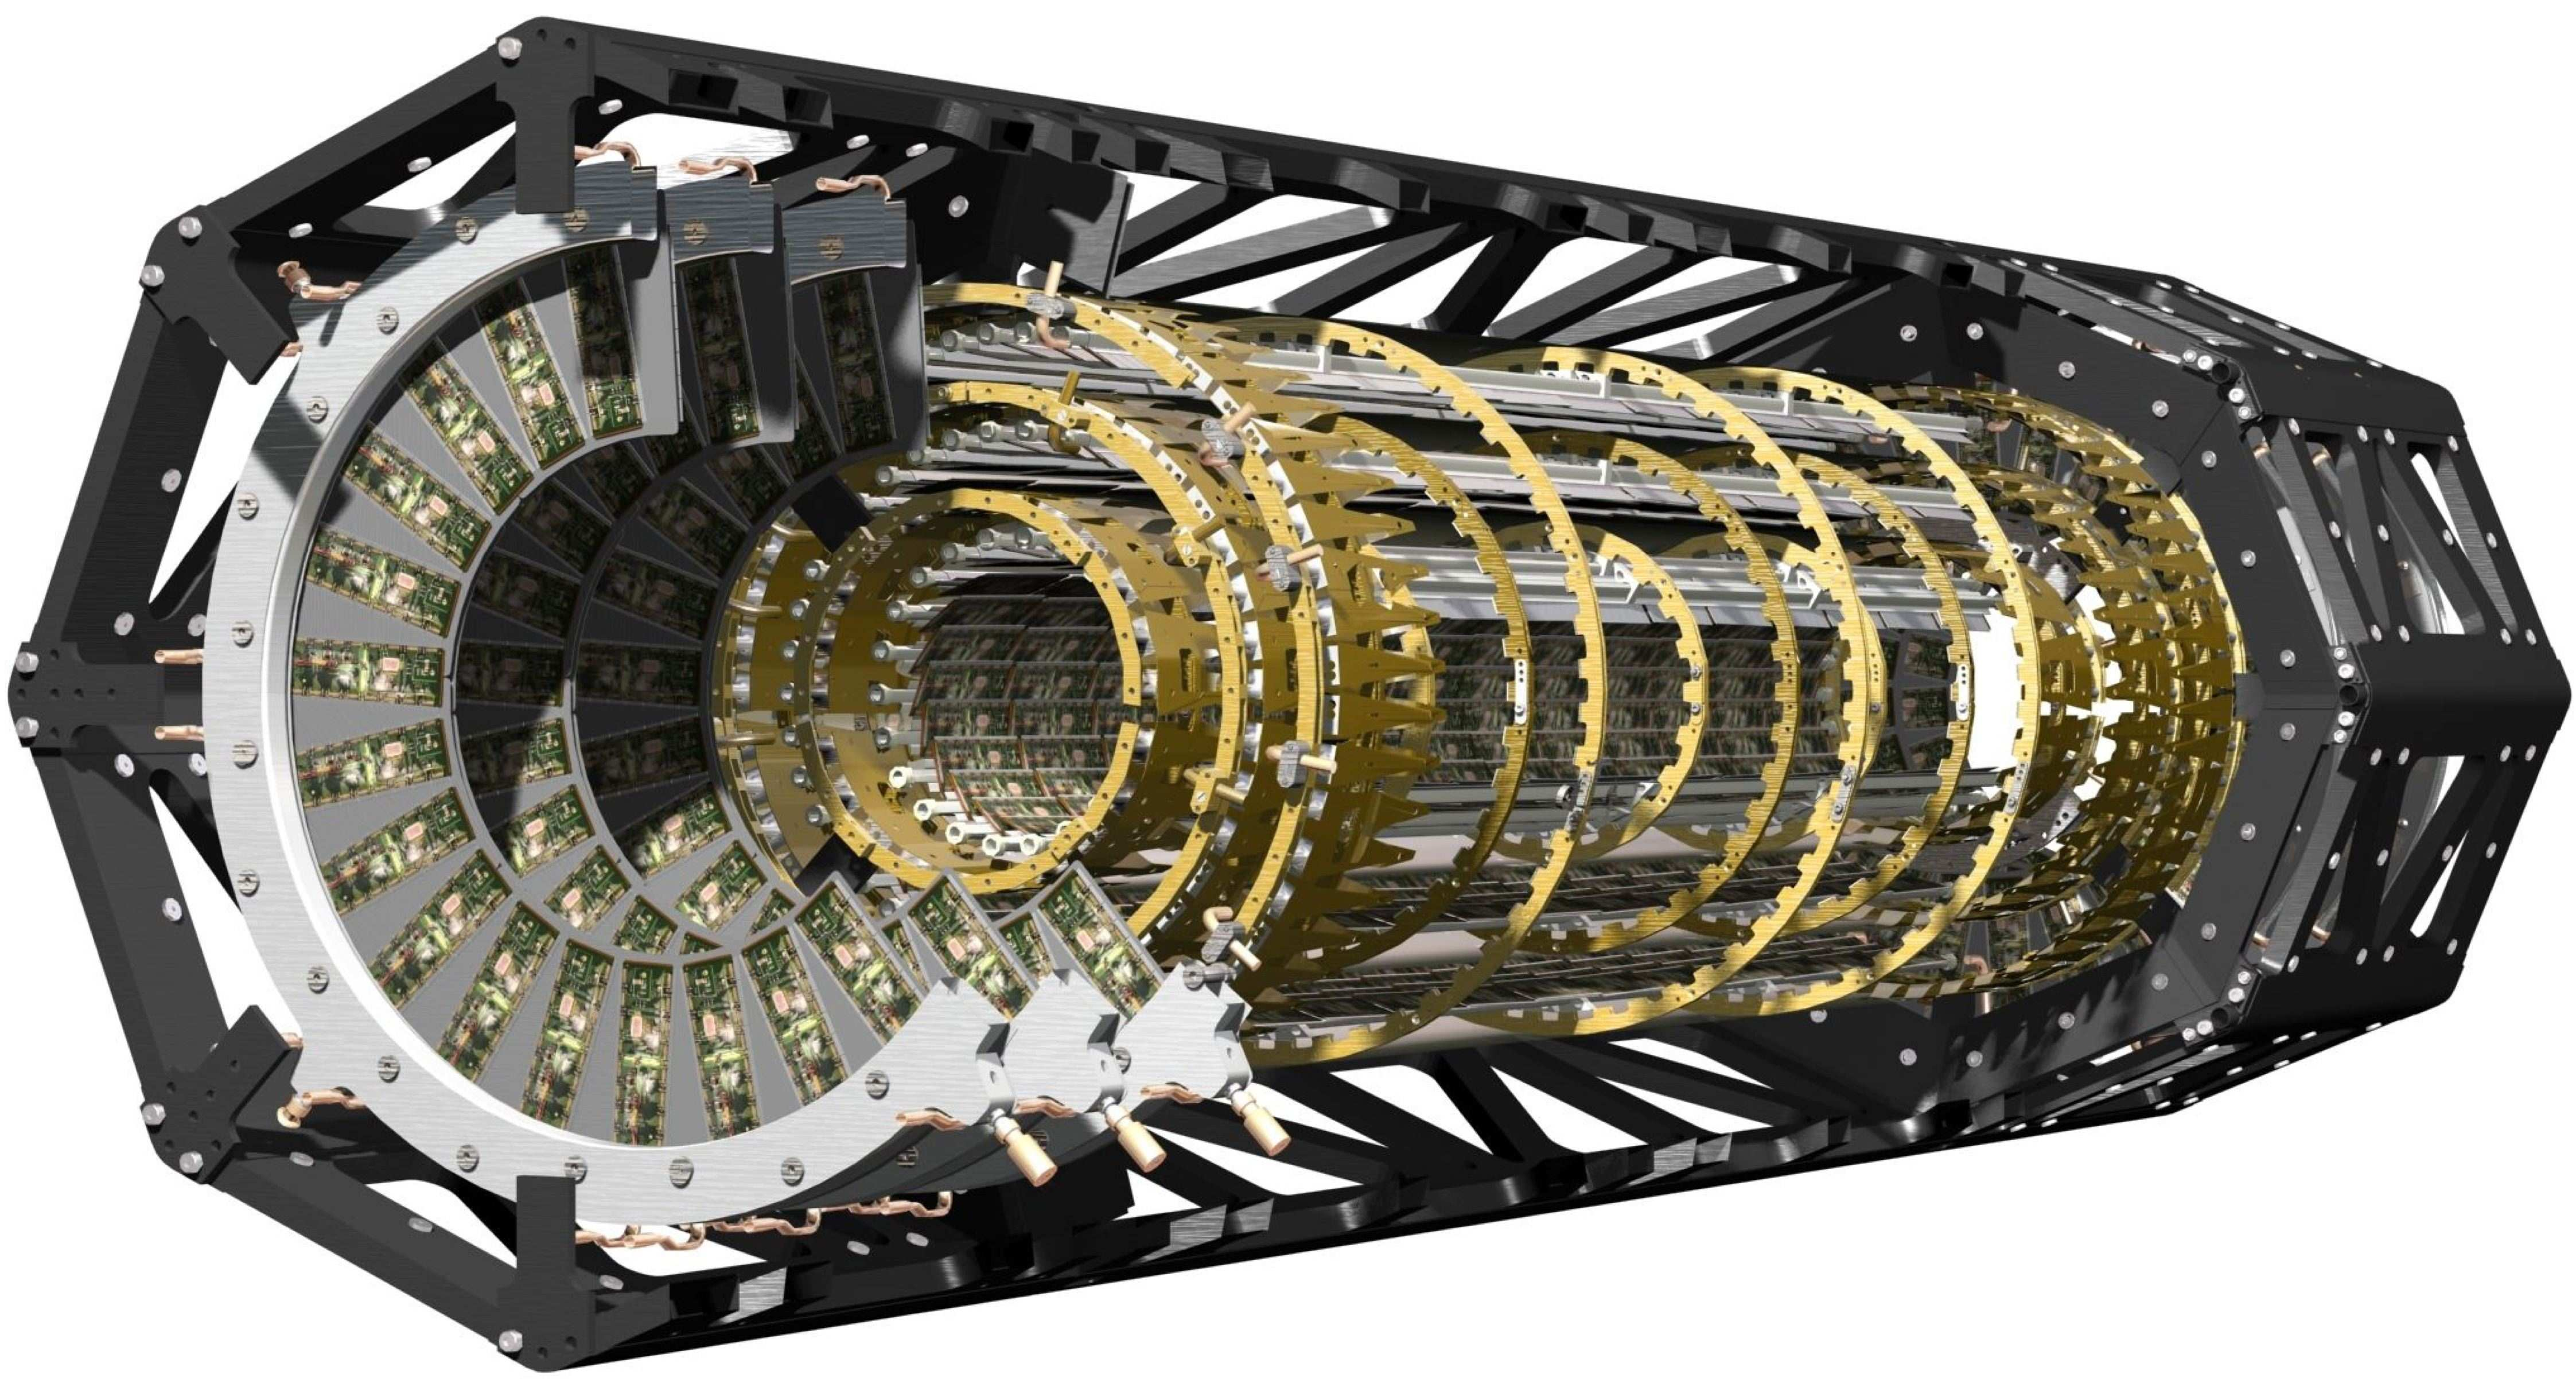
\includegraphics[width=\fullfig]{figures/pixel_overview.pdf}
\caption{}
\label{fig:pixel_overview}
\end{figure}

The innermost layer, the \ac{IBL}, was added during the long shutdown before Run 2, and provides the fourth track measurement.
It was inserted directly into the existing pixel detector by removing the existing beam pipe and replacing it with a significantly smaller version.
This insertion can be seen in action in Figure~\ref{fig:ibl_insertion}, which emphasizes the extreme precision required to place the the 70 cm long layer with only 2 mm of clearance.
The \ac{IBL} was commissioned to provide continued tracking robustness and high precision in the higher luminosity environment of Run 2~\cite{ibl_tdr}.
The proximity of this layer to the collisions necessitated an even higher granularity and better radiation hardness than the other pixel layers.
And the strict space requirements to add an active sensing layer so close to the interaction point required a sensor chip with a much higher active area and a larger overall area per chip.
These requirements led to the development of a new chip type, the FE-I4 (compared to the FE-I3 chips used in the original pixel detector) with improved radiation hardness and a larger active footprint of 90\%.
The \ac{IBL} is comprised of 448 of these individual chips arranged in 14 staves, with 26,880 pixels per chip and a chip size of 18.5 mm x 41.3 mm x 200 \um.
The staves, like in the other layers of the pixel detector, are offset by 14\textdegree to provide full azimuthal coverage.
This arrangement can be seen in Figure~\ref{fig:ibl_geometry}, which shows two computer-generated images of the \ac{IBL} geometry and includes the some of the remaining pixel layers.


\begin{figure}[hbtp]
\centering
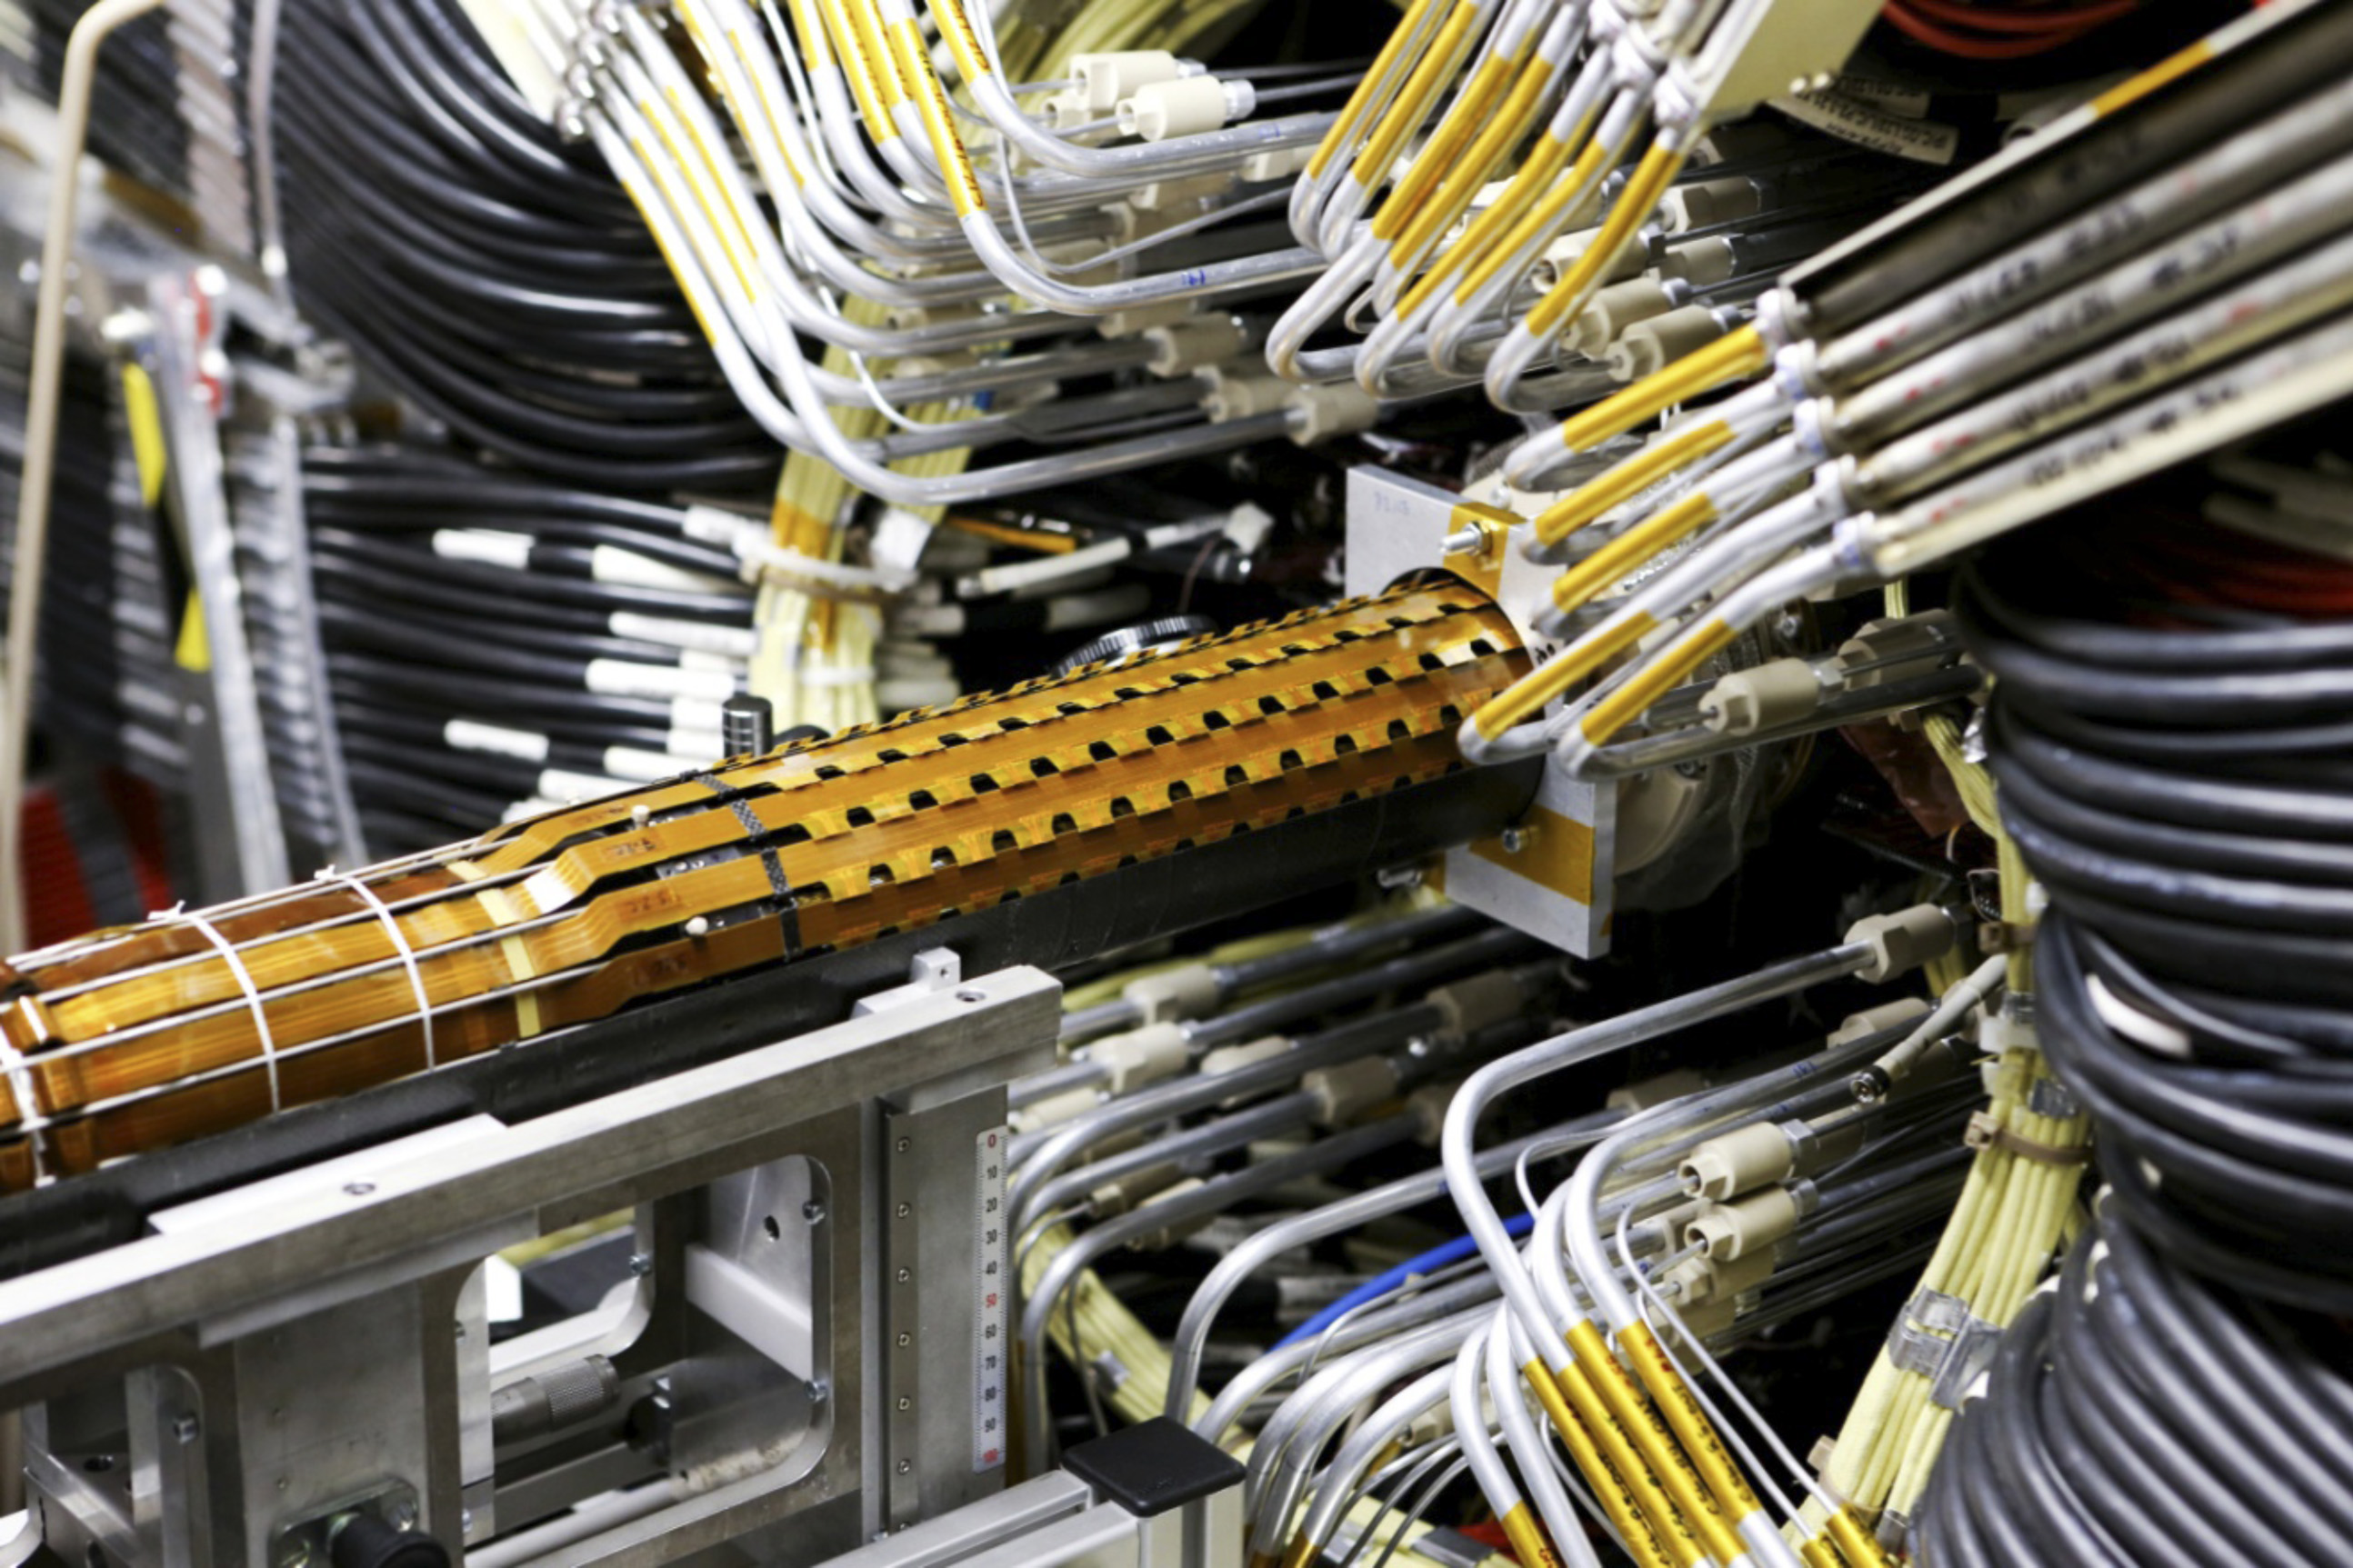
\includegraphics[width=\fullfig]{figures/ibl_insertion.jpg}
\caption{An image of the insertion of the \ac{IBL} into the current pixel detector.}
\label{fig:ibl_insertion}
\end{figure}


\begin{figure}[hbtp]
\centering
\subfloat[]{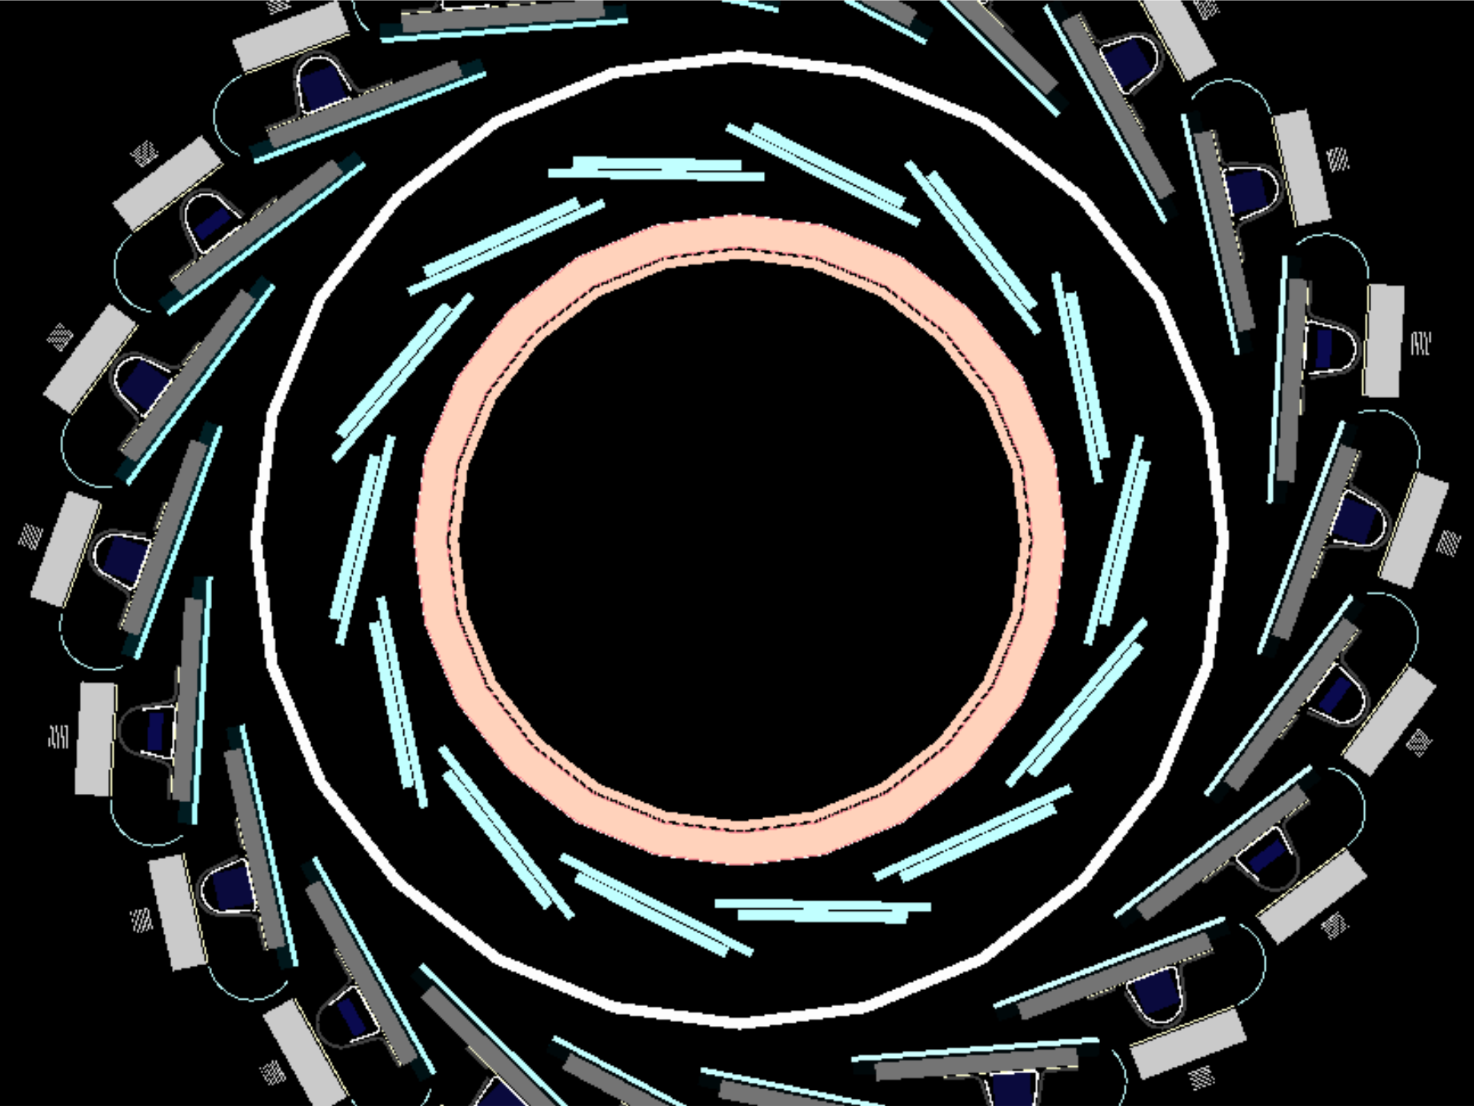
\includegraphics[width=\halffig]{figures/ibl_transverse.png}}\\
\subfloat[]{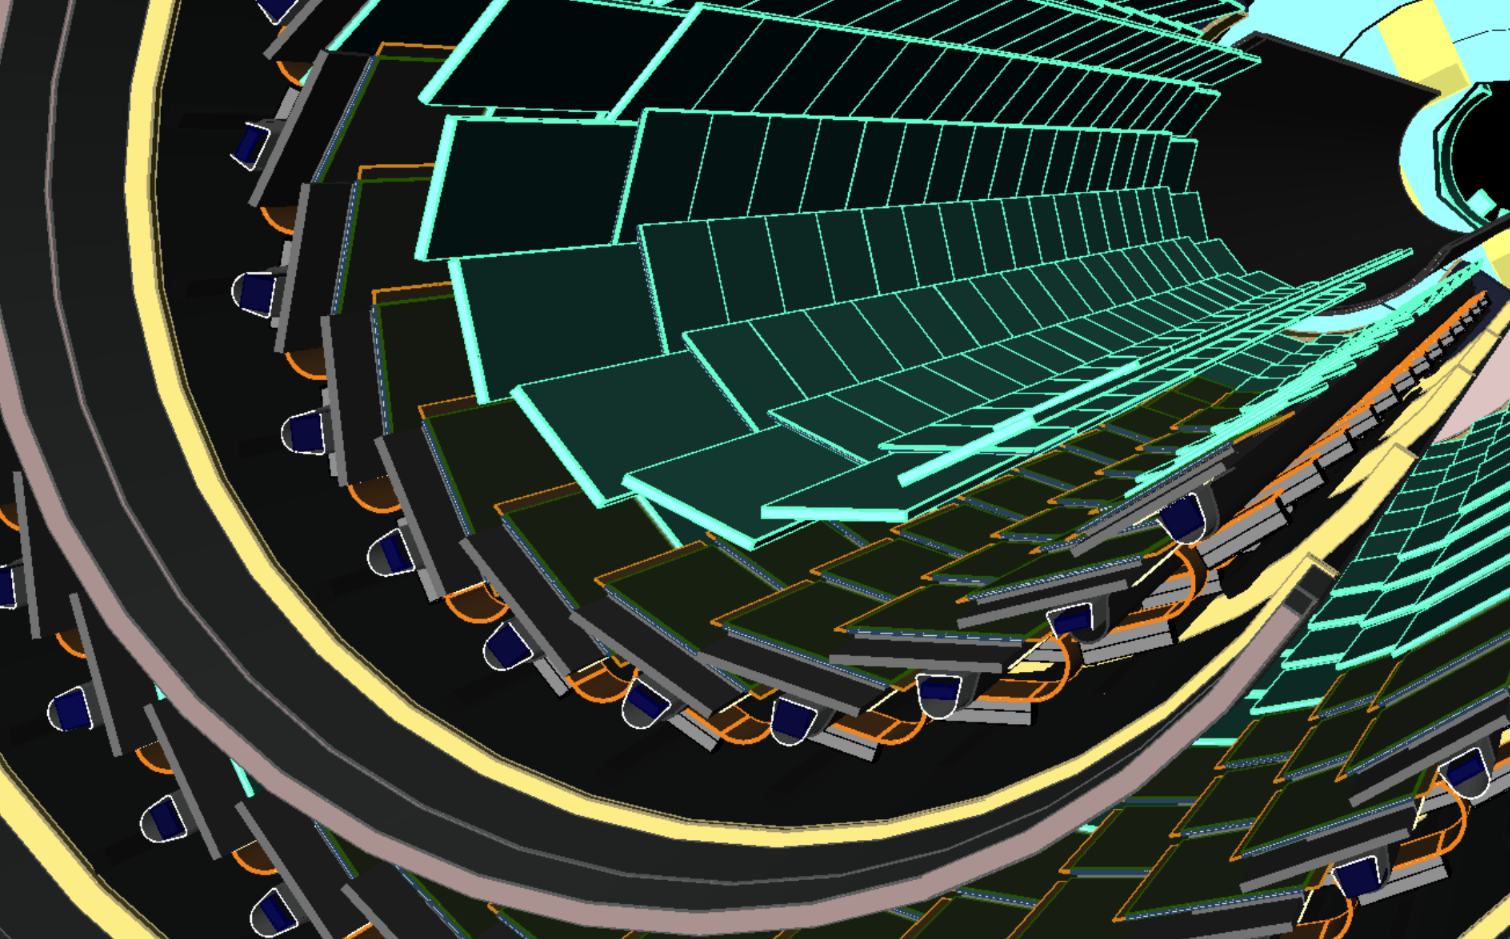
\includegraphics[width=\halffig]{figures/ibl_longitudinal.png}}
\caption{A three-dimensional computer-generated image of the geometry of the \ac{IBL} with a view (a) mostly transverse to the beam pipe (b) mostly parallel to the beam pipe.}
\label{fig:ibl_geometry}
\end{figure}

\subsection{Semiconductor Tracker}

The \ac{SCT}, the subdetector which immediately surrounds the Pixel detector, provides additional discrete measurements of the trajectory of a charged particle.
Because the \ac{SCT} is further away from the interaction point, the spatial resolution does not need to be as high as in the pixel detector, and so the \ac{SCT} uses micro-strips instead of pixels. 
Although pixels provide a more accurate measurement, the number of pixels and readout channels required to cover the cylidrical area at the radius of the \ac{SCT} layers would be prohibitively complicated and expensive.

Each individual silicon strip sensor contains 768 individual readout strips with a total area of 6.36 cm x 6.40 cm and a pitch of 80 \um. 
Pairs of these sensors are then bonded together to form a combined strip with a length of 12.8 cm.
Two of these combined strips are then placed back to back with a relative tilt of 40 mrad.
This geometry is illustrated in an exploded-out view in Figure~\ref{fig:sct_geometry}.
The purpose of angular offset of the consecutive layers is to allow the strip sensor areas to more accurately measure the position of a particle by comparing the overlap of the two strips which were traversed by a track.

\begin{figure}[hbtp]
\centering
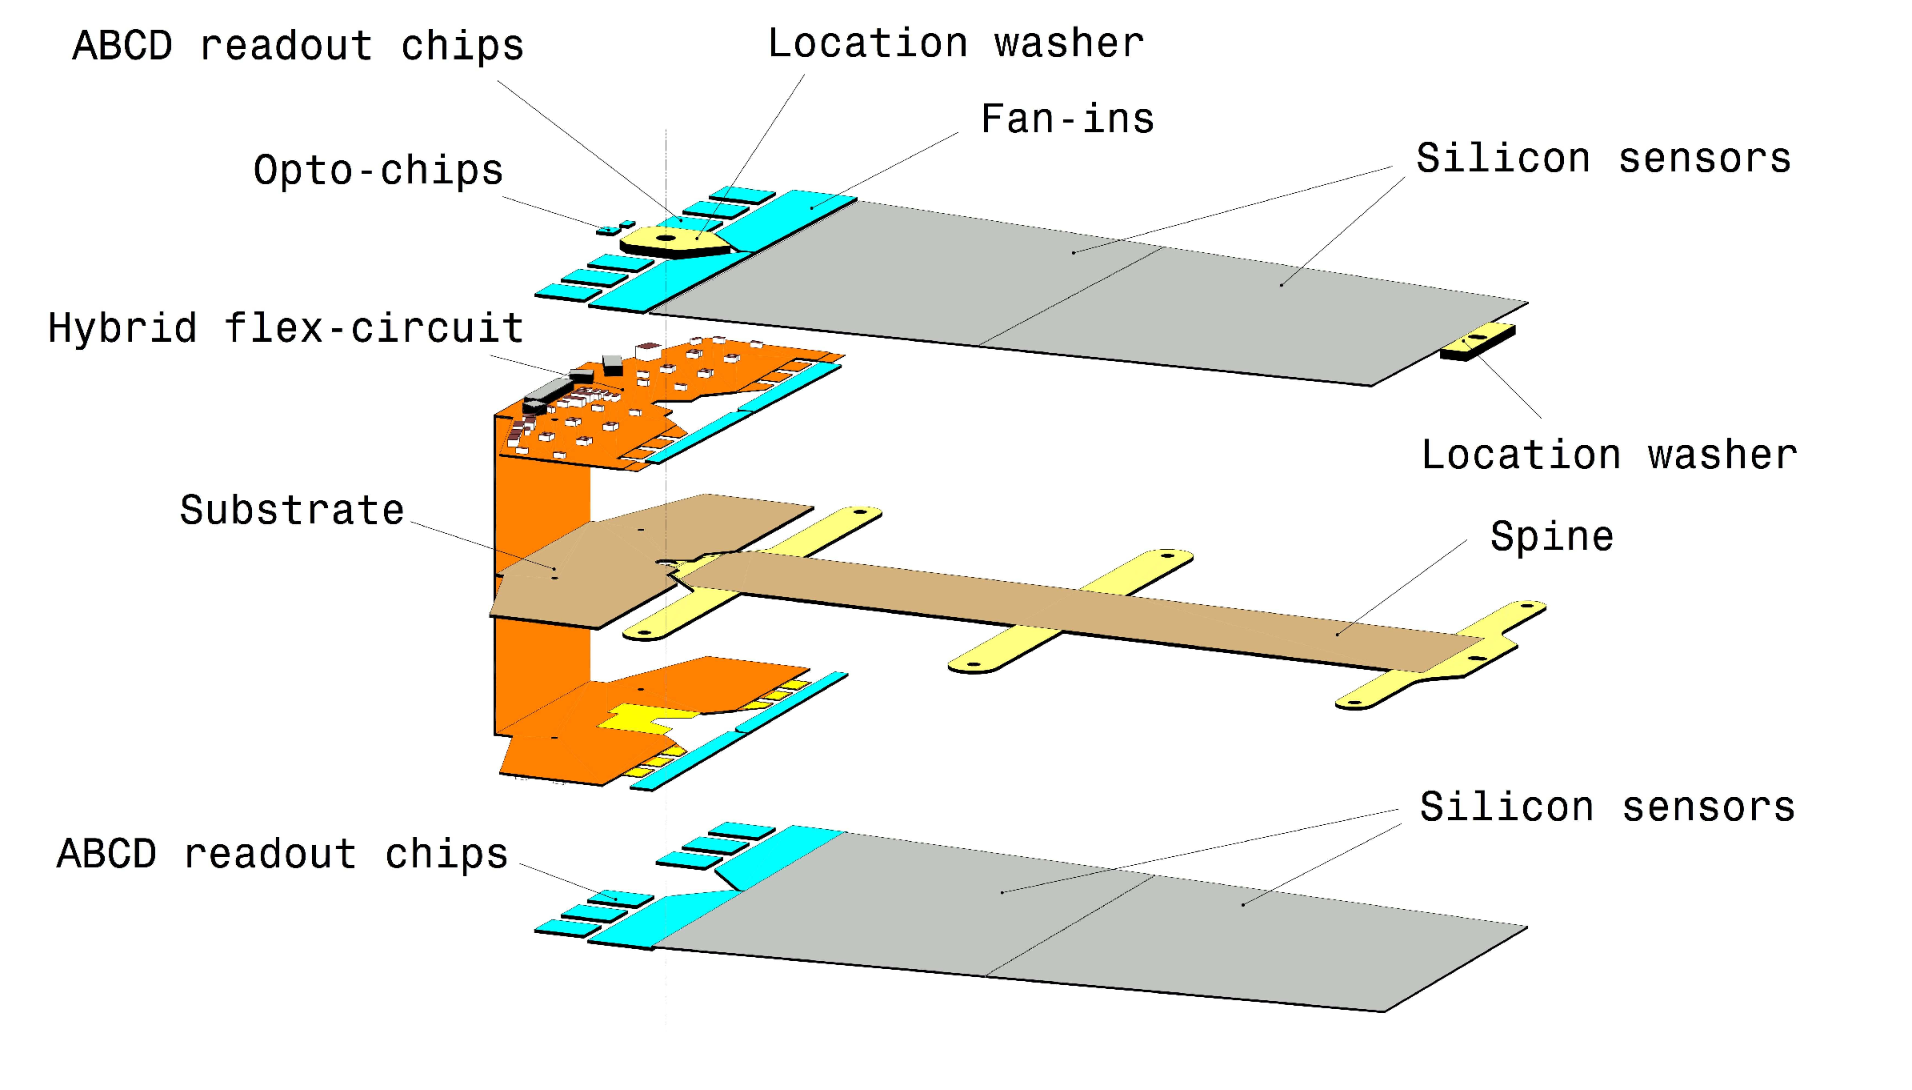
\includegraphics[width=\fullfig]{figures/sct_geometry.png}
\caption{An exploded view of the geometry of the \ac{SCT} double layers in the barrel region.}
\label{fig:sct_geometry}
\end{figure}

Four of these double layers are placed in the barrel region, with radii of 284 mm, 355 mm, 427 mm, and 498 mm. 
Together these layers provide eight additional measurements for each track that traverses the central $|\eta|$ region.
In the endcap region, the layers are arranged in wheels, with the double layers similarly offset to provide improved resolution.
With these configurations, the \ac{SCT} achieves a spatial resolution of 17 \um in the $r-\phi$ direction and 580 \um in the $z$ direction.

\subsection{Transition Radiation Tracker}

The final component of the inner detector, the \ac{TRT}, provides continuous tracking using straw drift tubes.
The tubes are made of Kapton and aluminum with a diameter of 4 mm and are filled with a gas mixture of 70\% Xe, 27\% CO\tsub{2}, and 3\% 0\tsub{2}. 
At the center of each tube is a gold-plated anode tungsten wire 30 \um in diameter.
When a charged particle passes through these tubes, it ionizes the gas within.
The ions produced drift in the electric field established between the wire and the tube wall, and the large electric field near the wire produces avalanche multiplication and results in an electric current on the wire that is read out by the electronics and provides a track measurement.
The time it takes the ionization to drift to the wire can be used to estimate the distance from the wire that the particle passed through the tube; this gives a resolution on the distance of approximately 130\um.
Combining several such measurements between consecutive hits in the \ac{TRT} tubes allows the trajectory of the particle to be reconstructed.

In addition to the continuous tracking, the detector can use transition radiation produced when a particle passes between the layers to distinguish between electrons and heavier charged particles.
The space between the tubes is filled with CO\tsub{2}, and so has a different dielectric constant than the gas within the tubes which contains Xe.
At the transition between those media, a relativistic particle emits radiation proportional to $\gamma$, so inversely proportional to mass at a fixed momentum.
The photons produced in this transition then produces an ionization cascade which is significantly larger than the signal for the minimally-ionizing charged particles.
To distinguish between these two cases, the \ac{TRT} defines two signal thresholds, a low threshold for the typical signal produced by a \ac{MIP} and a high threshold for the the signal produced by transition radiation.
A high momentum electron is expected to produce approximately 7 to 10 high threshold hits as it traverses the \ac{TRT}, and thus these hits provide a way to distinguish electrons from other charged particles. 

The \ac{TRT} contains 351,000 tubes in total, divided between the barrel and endcap regions. 
In the barrel region, the tubes are 144 cm long and arranged in 73 layers parallel to the beampipe.
In the endcap region, the tubes are 37 cm long and arranged in 160 layers transverse to the beampipe.
These configurations can be seen in Figure~\ref{fig:id_slice} and Figure~\ref{fig:id_slice_long}. 
With this geometry the \ac{TRT} achieves a resolution of 130 \um  in the $r-\phi$ direction.

% ----------------------------------------

\section{Calorimetry}
\label{sec:calorimetry}

The combination of calorimeter systems used in \ac{ATLAS} can measure the energy of electrons, photons, hadrons, and hadronic jets with complete coverage up to $|\eta| < 4.9$ and across $\phi$.
Unlike the inner detector, the calorimeters are capable of measuring neutral particles.
To accomplish precision measurements of these particle types, the \ac{ATLAS} calorimeter system uses four individual calorimeters, a \ac{LAr} \acl{EM} calorimeter in the barrel region, a tile hadronic calorimeter in the barrel region, a \ac{LAr} hadronic endcap calorimeter, and a \ac{LAr} forward calorimeter.
Together these provide hermetic coverage for the \ac{ATLAS} detector.
The configuration of these calorimeters is illustrated in Figure~\ref{fig:calo_overview}. 
%Table~\ref{tab:calorimeter_parameters} summarizes the parameters of these systems.
\textbf{Note: I could make this section much longer. It might be nice to include a more complete description of showers for example. I will extend this section if their is space at the end.}

\begin{figure}[hbtp]
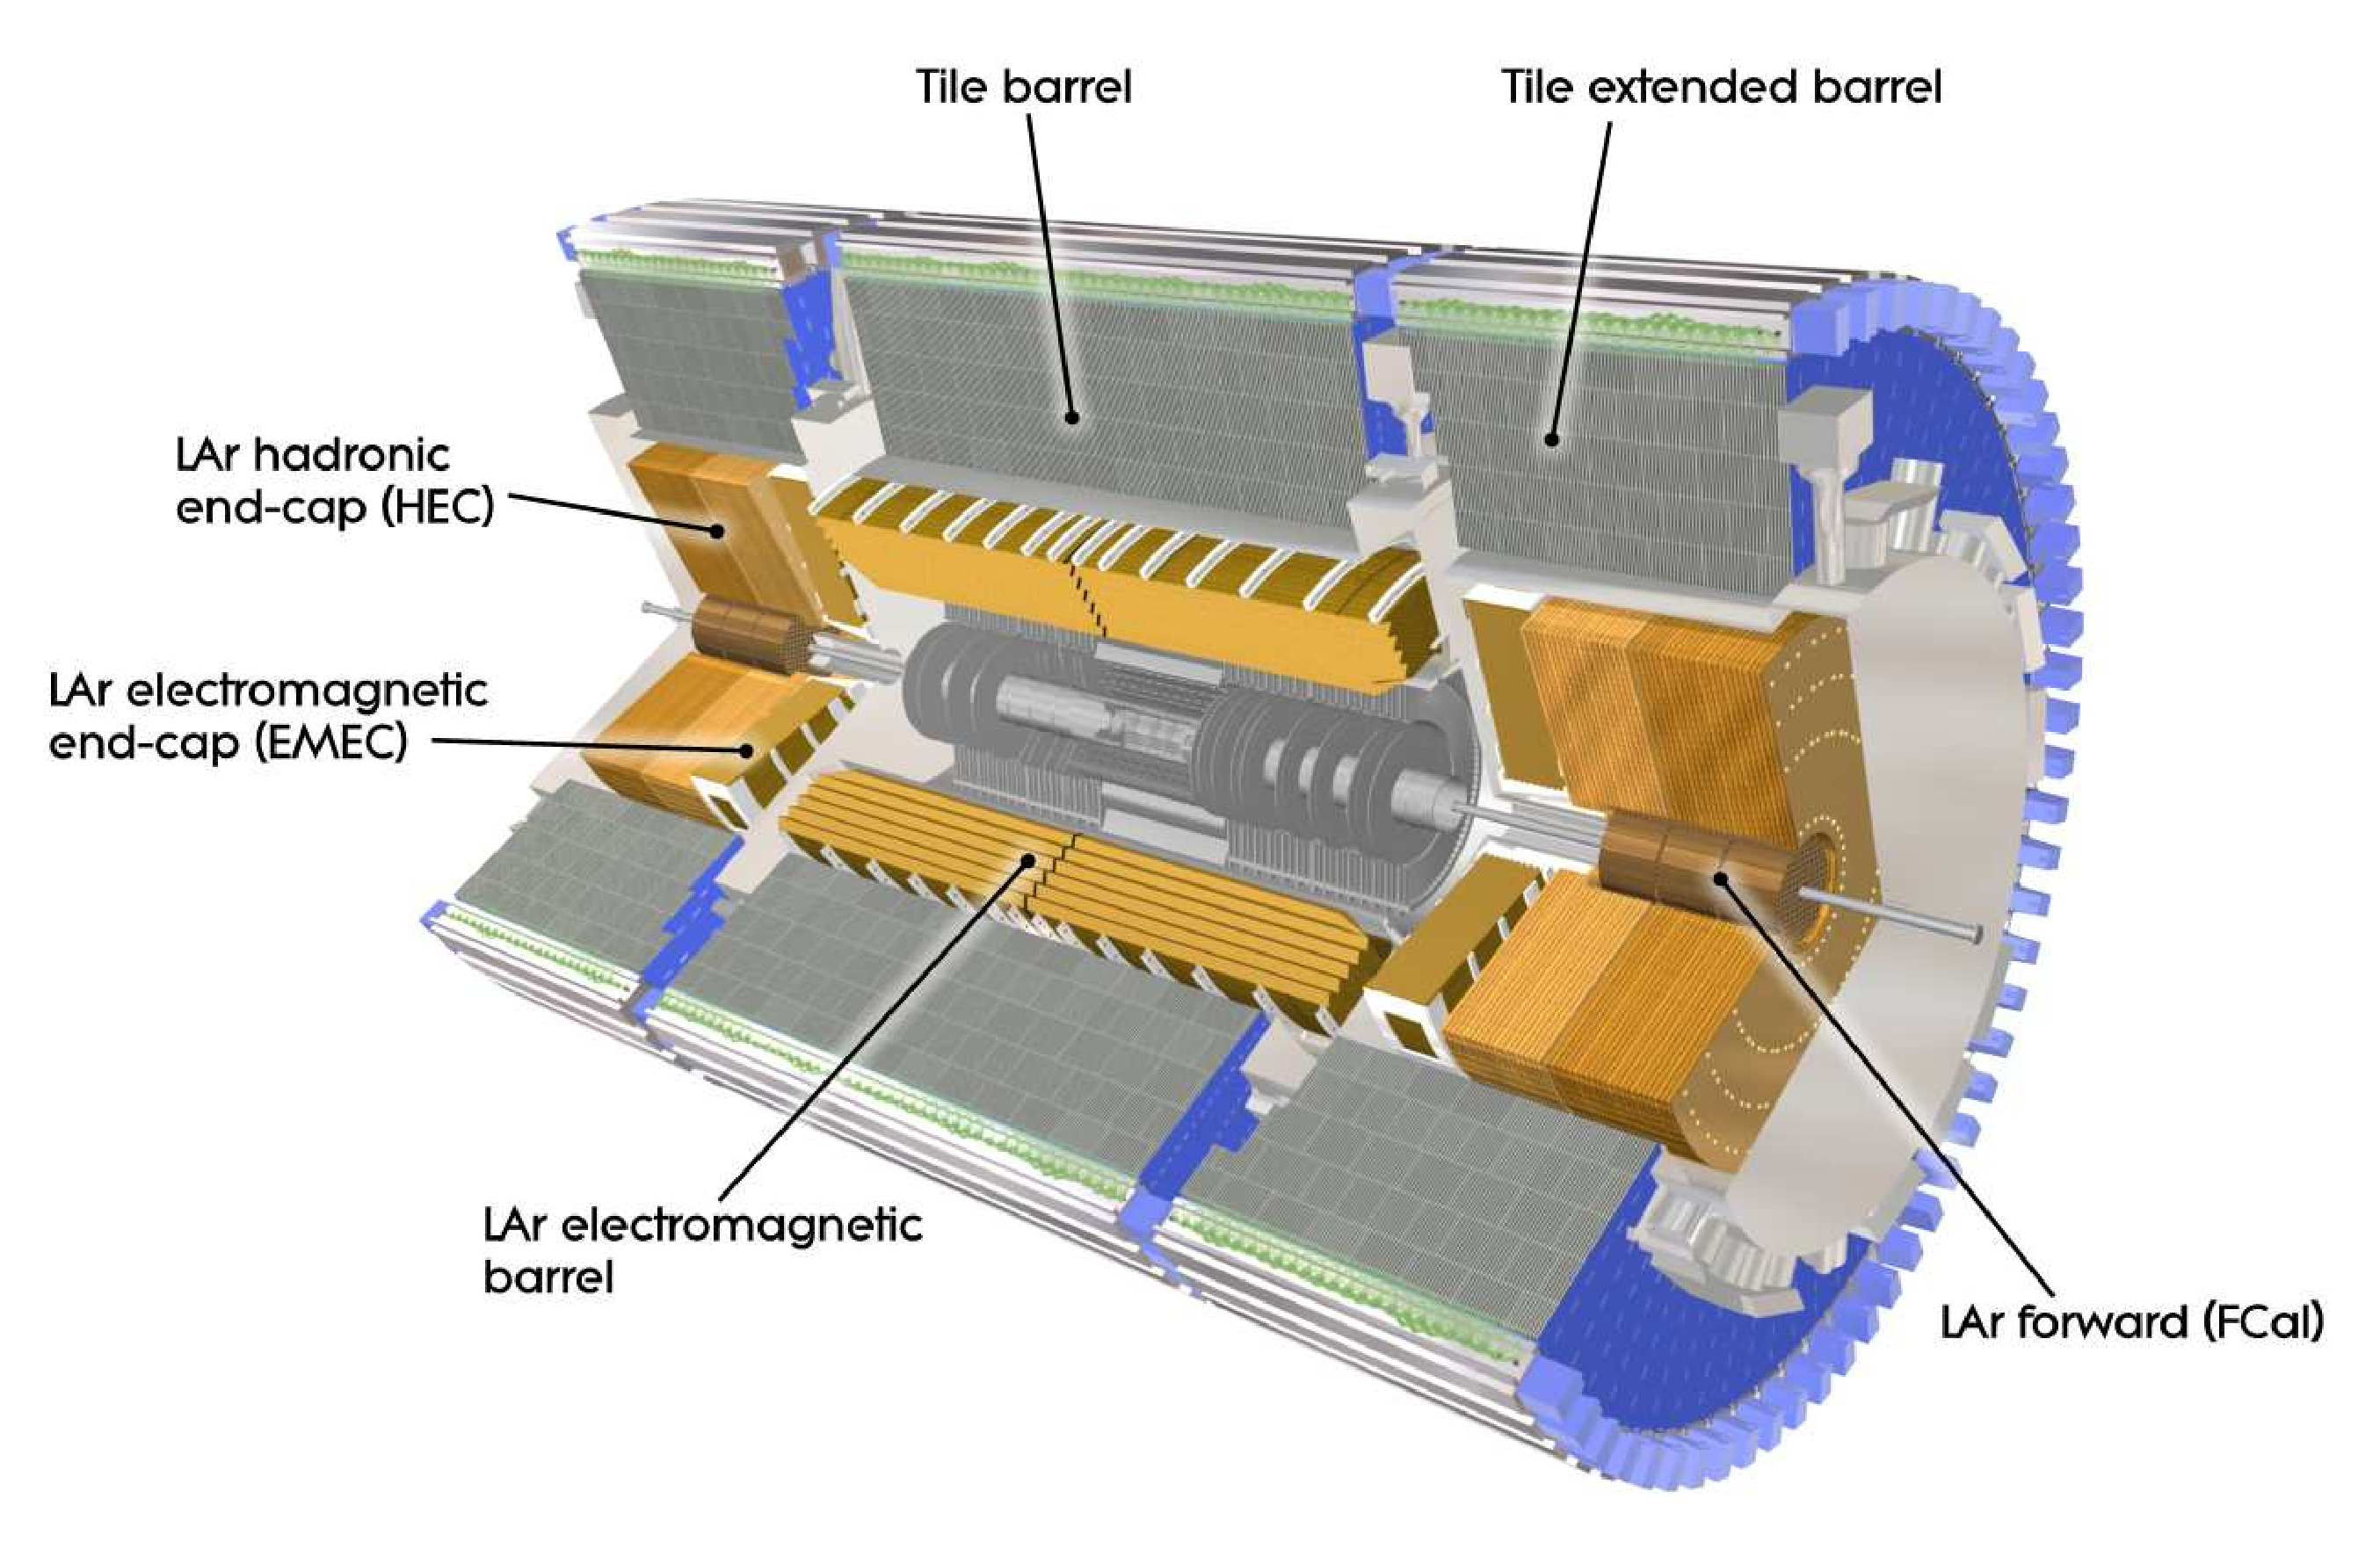
\includegraphics[width=\fullfig]{figures/calo_overview.pdf}
\caption{}
\label{fig:calo_overview}
\end{figure}

% This seems unnecessary, I will come back and add it if anyone asks for it.
%\begin{table}[hbtp]
%\begin{tabular}{lclll}
%\hline
%Component & Layers & Coverage & Granularity & Depth \\
%\hline
%\multicolumn{5}{c}{\ac{EM} Barrel Calorimeter}\\
%Layer 1 & 1 & $|\eta| < 1.475$ & 0.003 x 0.1 & 4.3 $X_0$ \\
%Layer 2 & 1 & $|\eta| < 1.475$ & 0.025 x 0.025 & 16 $X_0$ \\
%Layer 3 & 1 & $|\eta| < 1.475$ & 0.05 x 0.025 & 2 $X_0$ \\
%\multicolumn{5}{c}{\ac{EM} Endcap Calorimeter}\\
%Layer 1 & 1 & $1.375 < |\eta| < 3.2$ & 0.003 x 0.1 & 4.0 $X_0$ \\
%Layer 2 & 1 & $1.375 < |\eta| < 3.2$ & 0.025 x 0.025 & 20 $X_0$ \\
%Layer 3 & 1 & $1.5 < |\eta| < 2.5$ & 0.05 x 0.025 & 2 $X_0$ \\
%\multicolumn{5}{c}{Hadronic Tile Calorimeter}\\
%\multicolumn{5}{c}{EM Barrel Calorimeter}\\
%\multicolumn{5}{c}{EM Barrel Calorimeter}\\
%\hline
%\end{tabular}
%\caption{The granularity is measured in units of $\Delta\eta x \Delta\phi$.}
%\end{table}

The calorimeters are designed to absorb and measure the energy carried by a particle, and completely stop the particle's propagation in the process.
This requires a significant amount of material to provide interactions.
These interactions then produce secondary particles, which can produces secondary particles in turn, and thus form a cascade of particles called an \ac{EM} or hadronic shower, depending on the governing mechanism.
Electromagnetic and hadronic showers have very different properties and require different technologies to measure them accurately.
All of the calorimeters in the \ac{ATLAS} calorimeter system are sampling calorimeters, that is they use alternating layers of absorbing and active material.
The dense absorbing layers initiate the showers while the active layers measure the energy of the produced particles.
A fraction of the energy is lost in the inactive layers, so the energy measurement from the active layers has to be corrected to estimate the actual energy of the particle.

The \ac{EM} calorimeter provides around 20 radiation lengths ($X_0$) while the hadronic calorimeter provides around 10 interaction lengths ($\lambda_0$. 
As mentioned previously, radiation lengths measure the distance over which an electromagnetically interacting particle loses a characteristic fraction of its energy.
Interaction lengths, on the other hand, measure the mean distance travelled by a hadronic particle before undergoing a nuclear interaction~\cite{pdg}.
Figure~\ref{fig:calo_interactionlengths} show the radiation lengths in the layers of the \ac{EM} calorimeter in the barrel region as well as the interaction lengths for all calorimeters.


\begin{figure}[hbtp]
\subfloat[]{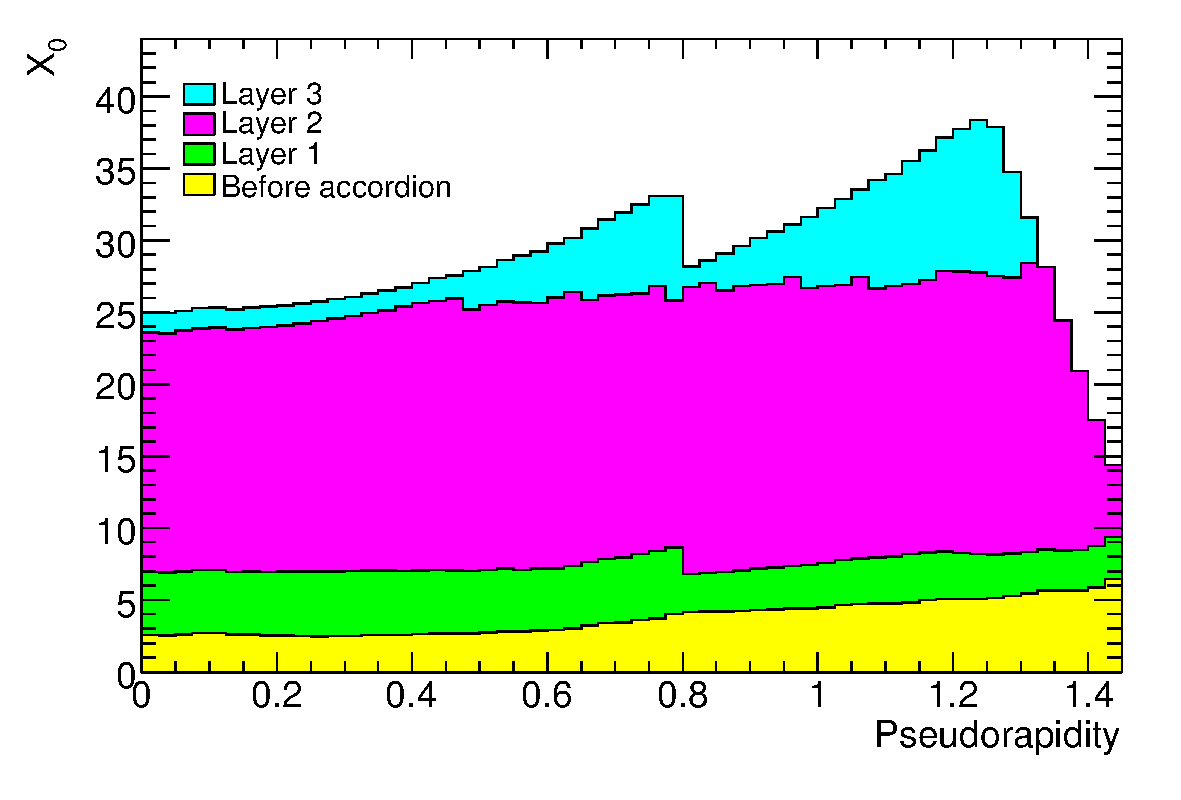
\includegraphics[width=\halffig]{figures/calo_radiationlengths.pdf}}
\subfloat[]{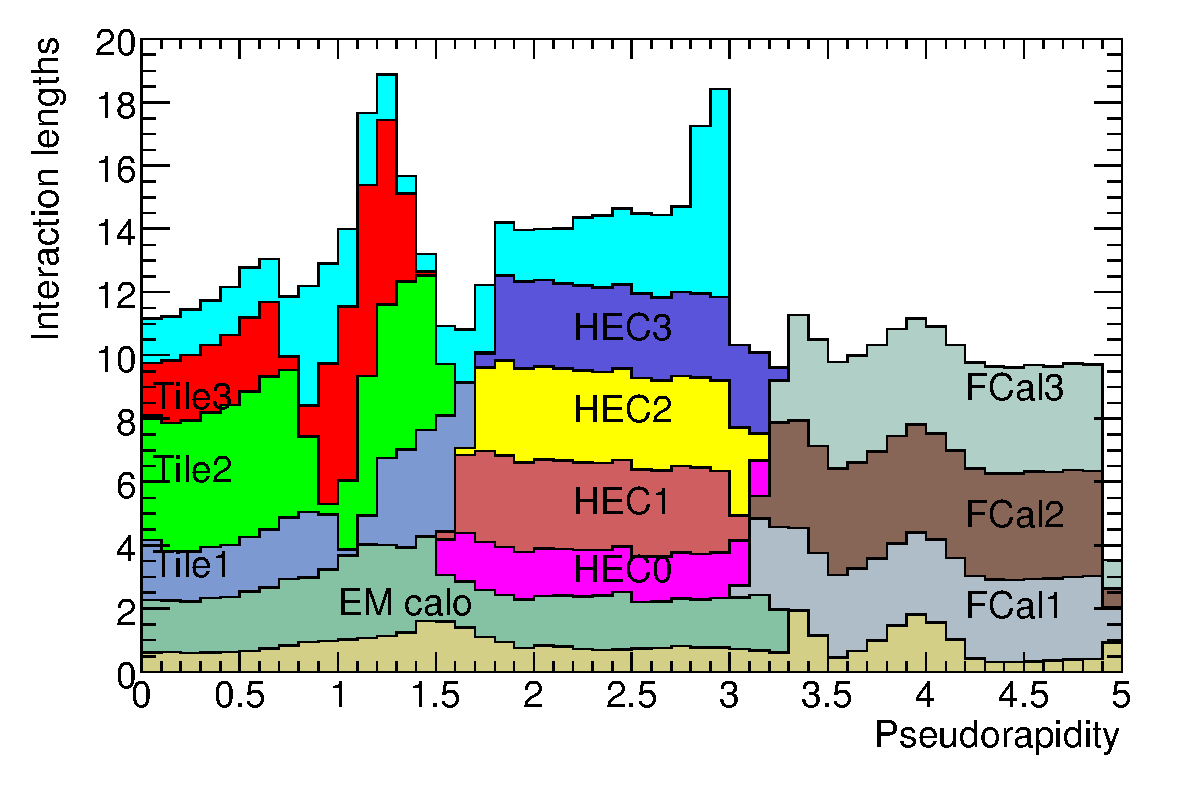
\includegraphics[width=\halffig]{figures/calo_interactionlengths.pdf}}
\caption{The depth of (a) the electromagnetic barrel calorimeter in radiation lengths and (b) all calorimeters in interaction lengths as a function of pseudorapidity.}
\label{fig:calo_interactionlengths}
\end{figure}

\subsection{Electromagnetic Calorimeter}

The electromagnetic calorimeters use alternating layers of \acl{LAr} and lead in an accordion shape. 
The accordion shape allows a construction that provides complete coverage in the $\phi$ direction while also providing many alternating layers for the a particle to pass through.
The configuration is detailed in Figure~\ref{fig:calo_barrel_schematic}.
When an electron or photon passes through the lead, it produces an electromagnetic shower.
The particles produced in those showers then pass into and ionize the \acl{LAr}; the ions produced can then be collected by an electrode in the \acl{LAr} layer to provide the actual energy measurement.

\begin{figure}[hbtp]
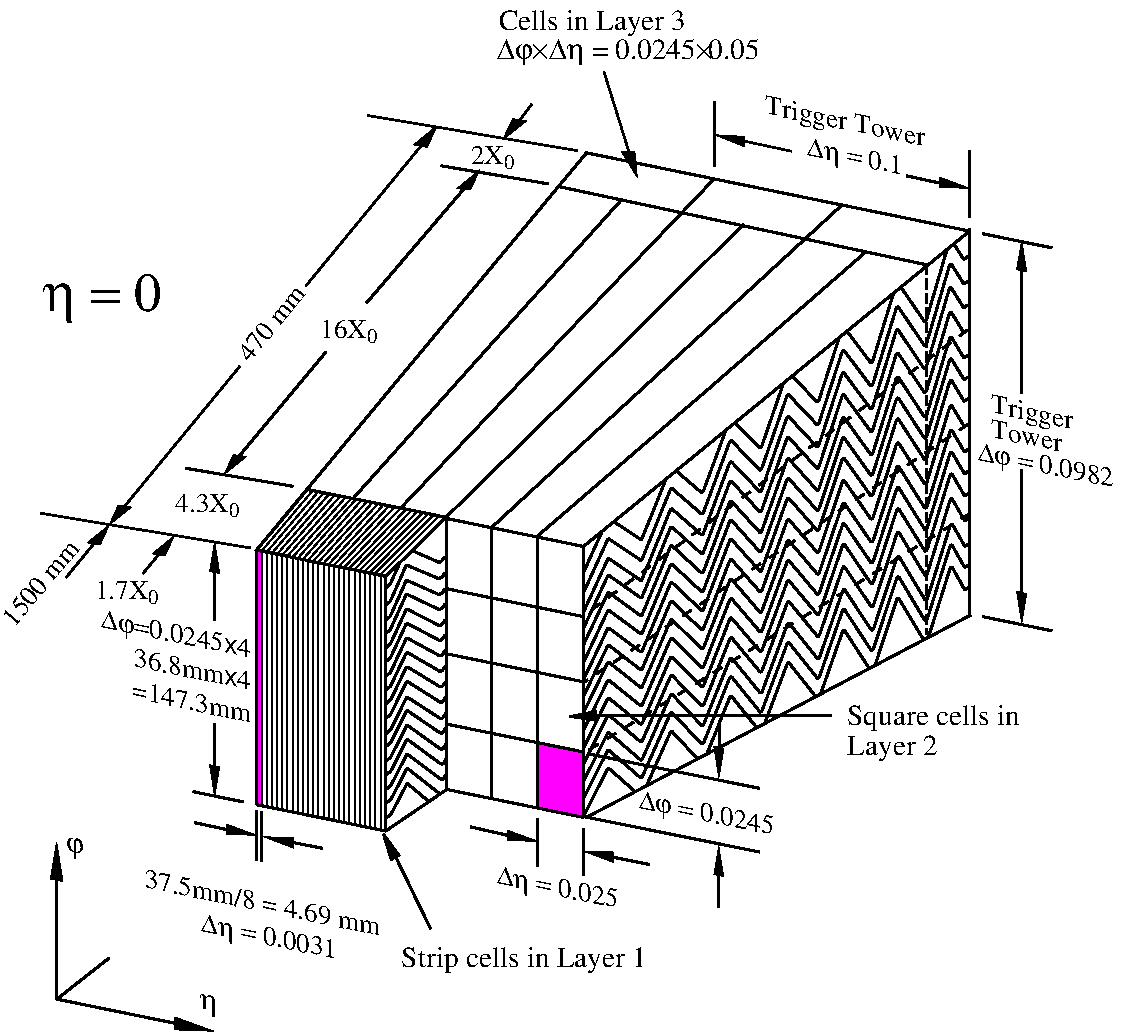
\includegraphics[width=\fullfig]{figures/calo_barrel_schematic.pdf}
\caption{A schematic of the \ac{LAr} calorimeter in the barrel region, highlighting the accordion structure.}
\label{fig:calo_barrel_schematic}
\end{figure}

The barrel region is covered by a presampler and three separate sampling layers with decreasing segmentation.
The presampler is just a thin layer of \acl{LAr} which measures the energy of any electromagnetic showers which are initiated before the particle reaches the calorimeter due to interactions with the detector material.
The first layer is the strip layer, which has fine segmentation in $\eta$ to enhance the identification of shower shapes and to provide a precise $\eta$ measurement for reconstructing photons and electrons.
The strip layer has only 4 radiation lengths worth of material, and has a segmentation of $\Delta\eta = 0.003$ and $\Delta\phi = 0.1$. 
The second layer is also finely segmented, with a segmentation of $\Delta\eta = 0.025$ and $\Delta\phi = 0.025$, and a thickness of 16 $X_0$.
This layer is designed to contain an electromagnetic shower and to measure the majority of the energy for photons and electrons.
The third layer is only 2 $X_0$ thick and measures the energy of electromagnetic showers which leak out of the second layer, and helps to separate electromagnetic showers from hadronic showers. 
The structure of the \ac{LAr} endcap calorimeter is similar except that the layers are arranged parallel to the beampipe to measure energy deposits from high $\eta$ particles.

%\begin{figure}[hbtp]
%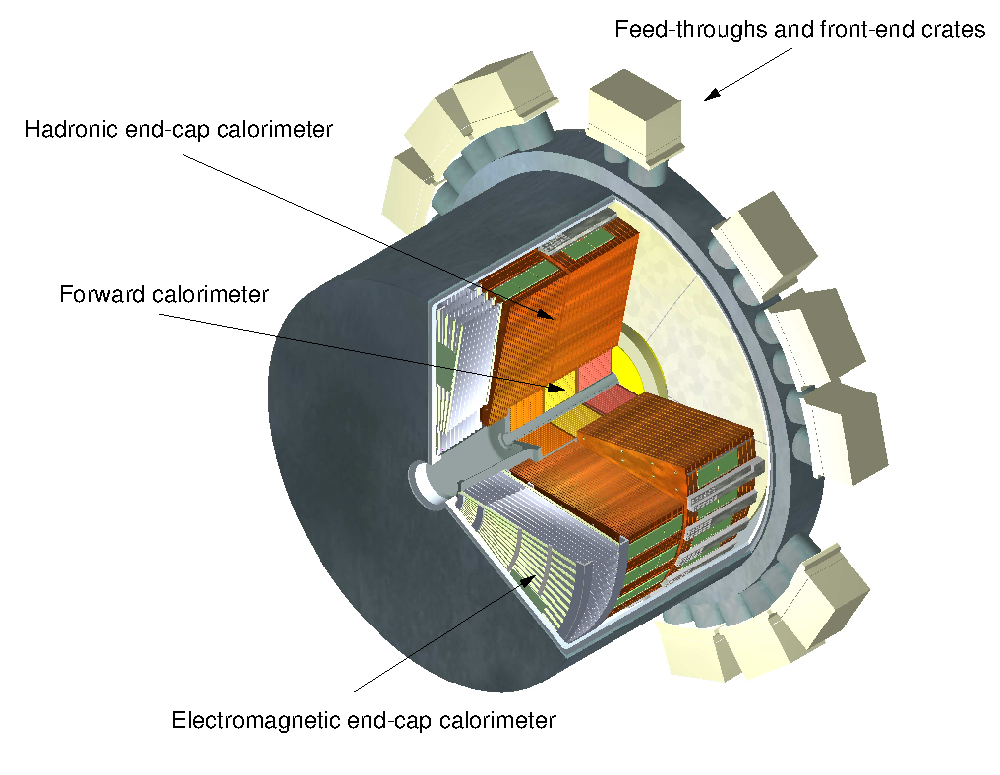
\includegraphics[width=\fullfig]{figures/calo_endcap_overview.pdf}
%\caption{}
%\label{fig:calo_endcap_overview}
%\end{figure}

\subsection{Hadronic Calorimeters}

The hadronic calorimeters use a few different technologies to satisfy the resolution demands in the different areas of the detector, and together they cover the region $|\eta| < 2.7$.
In the barrel region, for $|\eta| < 1.7$, the hadronic calorimeters are constructed of alternating tiles of steel and plastic scintillator. 
Like in the electromagnetic calorimeter, the dense layer initiates a shower (in this case the dense layer is the steel and the shower is hadronic) of particles which pass into and ionize the following layer.
The ioniziation in the plastic scintillator instead produces a light signal proportional to the amount of ionization produced by the shower, and this signal is measured using photomultipliers and provides the actual energy measurement.
The construction of a tile in the calorimeter is shown Figure~\ref{fig:hadronic_tile}, which highlights the alternating layers of steel and scintillator.

\begin{figure}[hbtp]
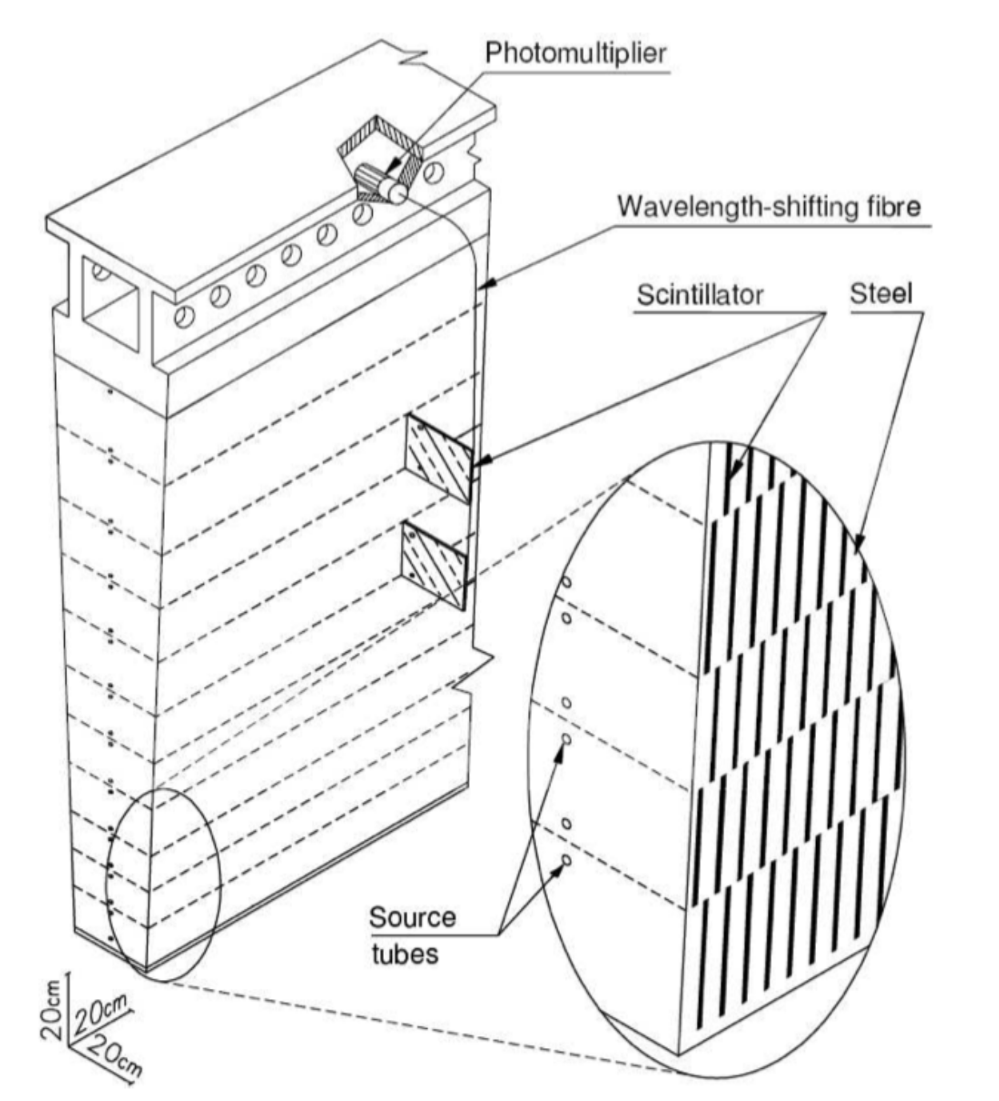
\includegraphics[width=\fullfig]{figures/hadronic_tile.png}
\caption{A schematic of a hadronic tile module which shows the alternating layers of steel and plastic scintillator.}
\label{fig:hadronic_tile.png}
\end{figure}

This tile calorimeter, as well as the remaining hadronic calorimeters, have a much coarser granularity than the electromagnetic calorimeters.
The high granularity is not needed for an accurate energy measurement, and the hadronic calorimeters are not designed to distinguish particle types like the electromagnetic calorimeters.
The tile granularity is approximately $\Delta\eta = 0.1$ and $\Delta\phi = 0.1$, and the segmentation in depth and $\eta$ is shown in Figure~\ref{fig:tile_segmentation}.

\begin{figure}[hbtp]
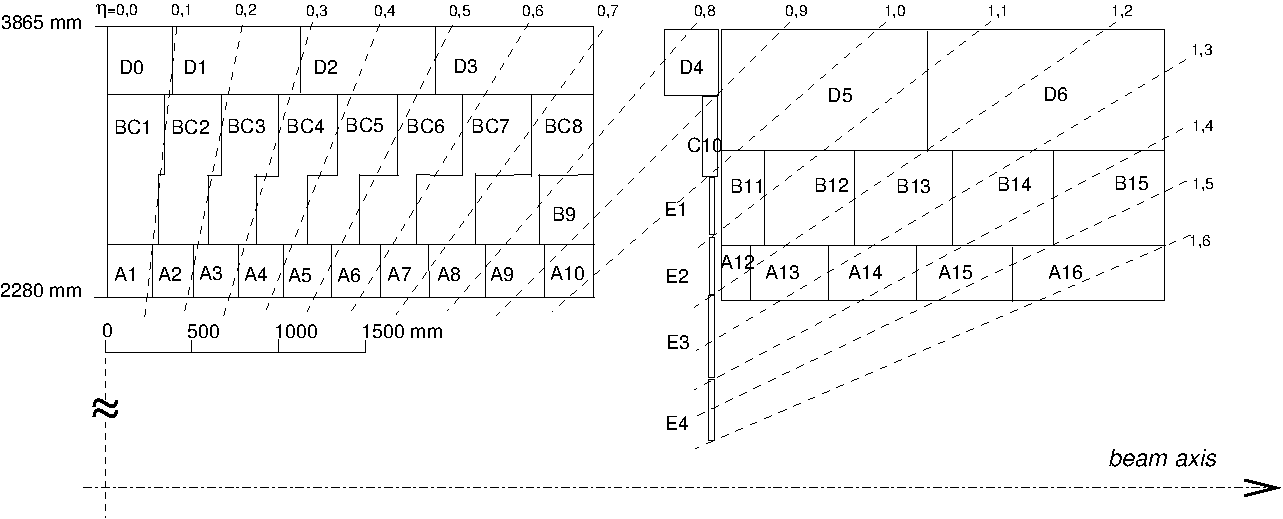
\includegraphics[width=\fullfig]{figures/tile_segmentation.pdf}
\caption{The segmentation in depth and $\eta$ of the tile-calorimeter modules in the central (left) and extended (right) barrels.}
\label{fig:tile_segmentation}
\end{figure}

The remaining hadronic calorimeters all use the same alternating, sampling structure but with different active and inactive materials.
The hadronic endcap calorimeter covers the range of $1.5 < |\eta| < 3.2$ and uses an inactive layer of copper and an active layer of \acl{liquid argon}.
The forward calorimeter covers the range of $3.1 < |\eta| < 4.9$ and uses a dense matrix of copper and tungsten filled with \acl{LAr}. 

% ----------------------------------------

\section{Muon Spectrometer}

Among \ac{SM} particles, only muons and neutrinos consistently pass through the calorimeters.
Because the neutrinos are also electrically neutral, there is no feasible option to measure them directly in \ac{ATLAS}.
The muons, on the other hand, are charged and are thus already measured as a track in the inner detector.
The muon spectrometer provides a way to consistently identify muon tracks and also a way to provide an additional measurement of their momentum.

The muon spectrometer contains four subdetectors that cover the barrel and endcap regions.
In the barrel region, the muon spectrometer uses a combination of \acp{RCP} and \acp{MDT} to provide both a coarse, fast measurement for triggering and a precise momentum measurement for offline event reconstruction.
Similarly, in the endcap region, the \acp{TGC}, \acp{MDT}, and \acp{CSC} allow for both triggering and precise measurements.
The \acp{CSC} are used only in the innermost layer of the endcap region between $2.0 < |\eta| < 2.7$ where the particle flux is too large for the \acp{MDT} to provide accurate measurements.
The overall layout of the muon systems are shown in the cut-away diagram in Figure~\ref{fig:muon_overview}, and Figure~\ref{fig:muon_side_schematic} shows a precise schematic of the layout of each of the detecting elements.
The geometric arrangement shown provides consistent coverage for muons produced up to $|\eta| < 2.7$, and takes full advantage of the bending of the muons in the toroidal magnetic field, described in Section~\ref{sec:magnetic_field}, to measure their momentum.
Figure~\ref{fig:muon_barrel_schematic} shows a cross-section of the arrangement of the muon spectrometer in the barrel; the layers are divided into eight small and eight large chambers that are overlapped to provide complete coverage in $\phi$. 


\begin{figure}[hbtp]
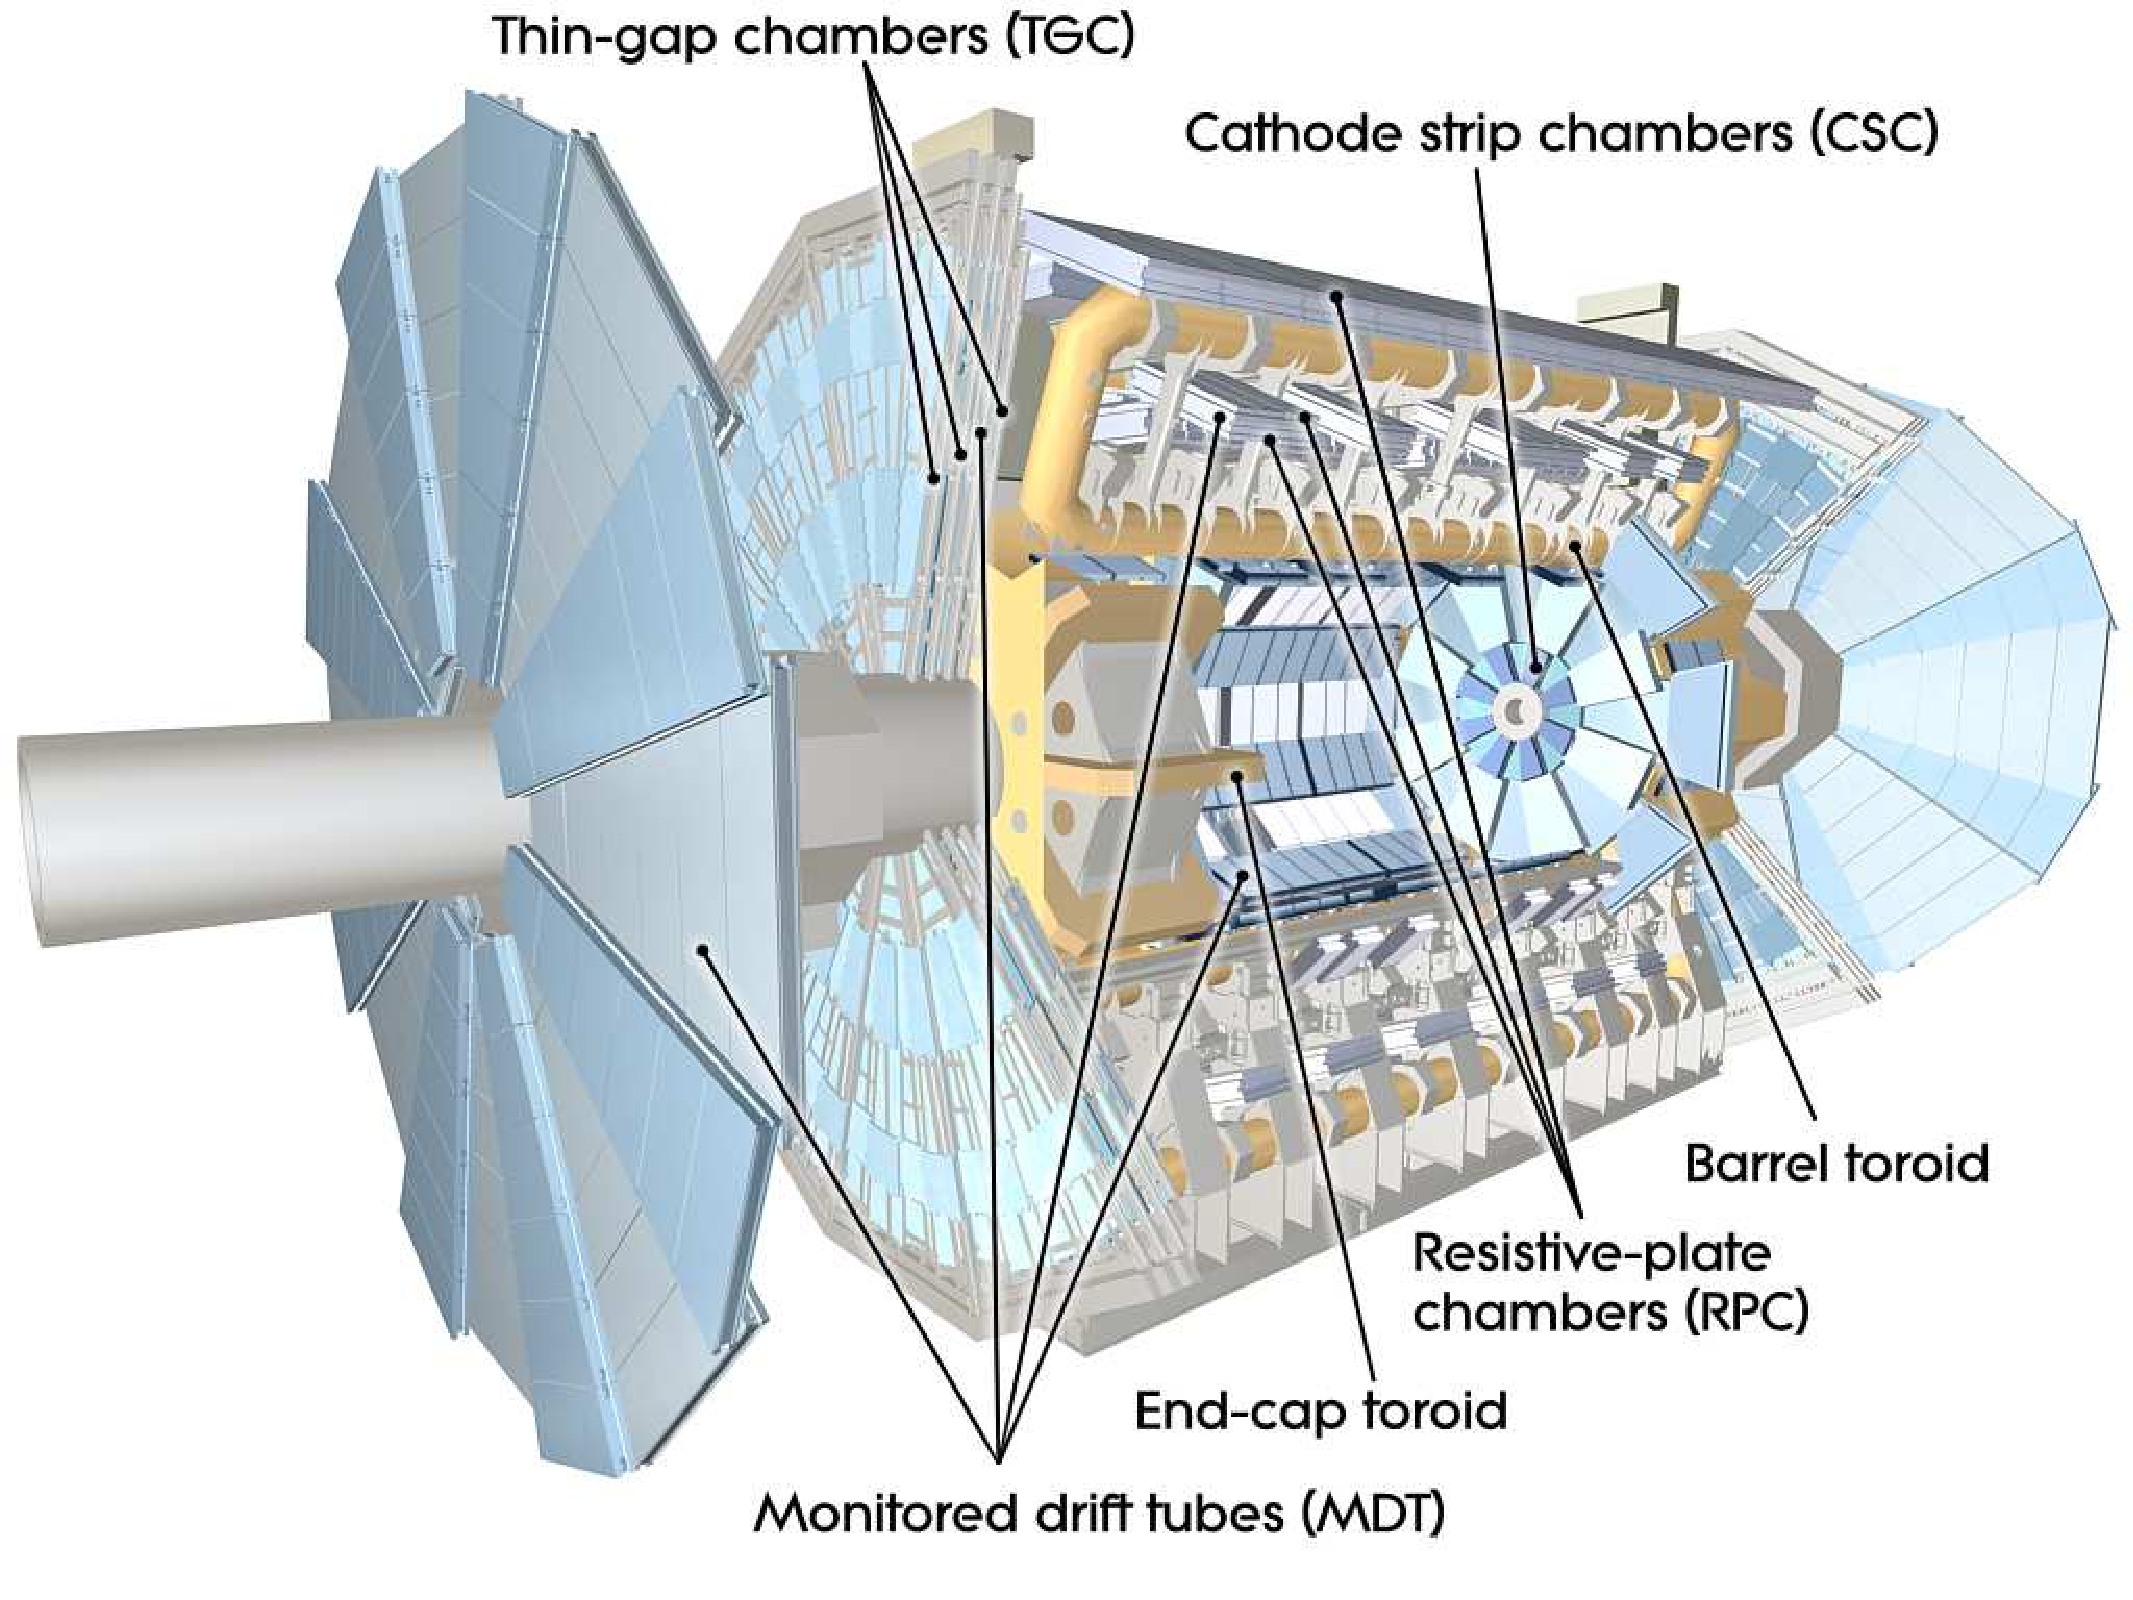
\includegraphics[width=\fullfig]{figures/muon_overview.pdf}
\caption{A cut-away diagram of the muon systems on \ac{ATLAS}.}
\label{fig:muon_overview}
\end{figure}

\begin{figure}[hbtp]
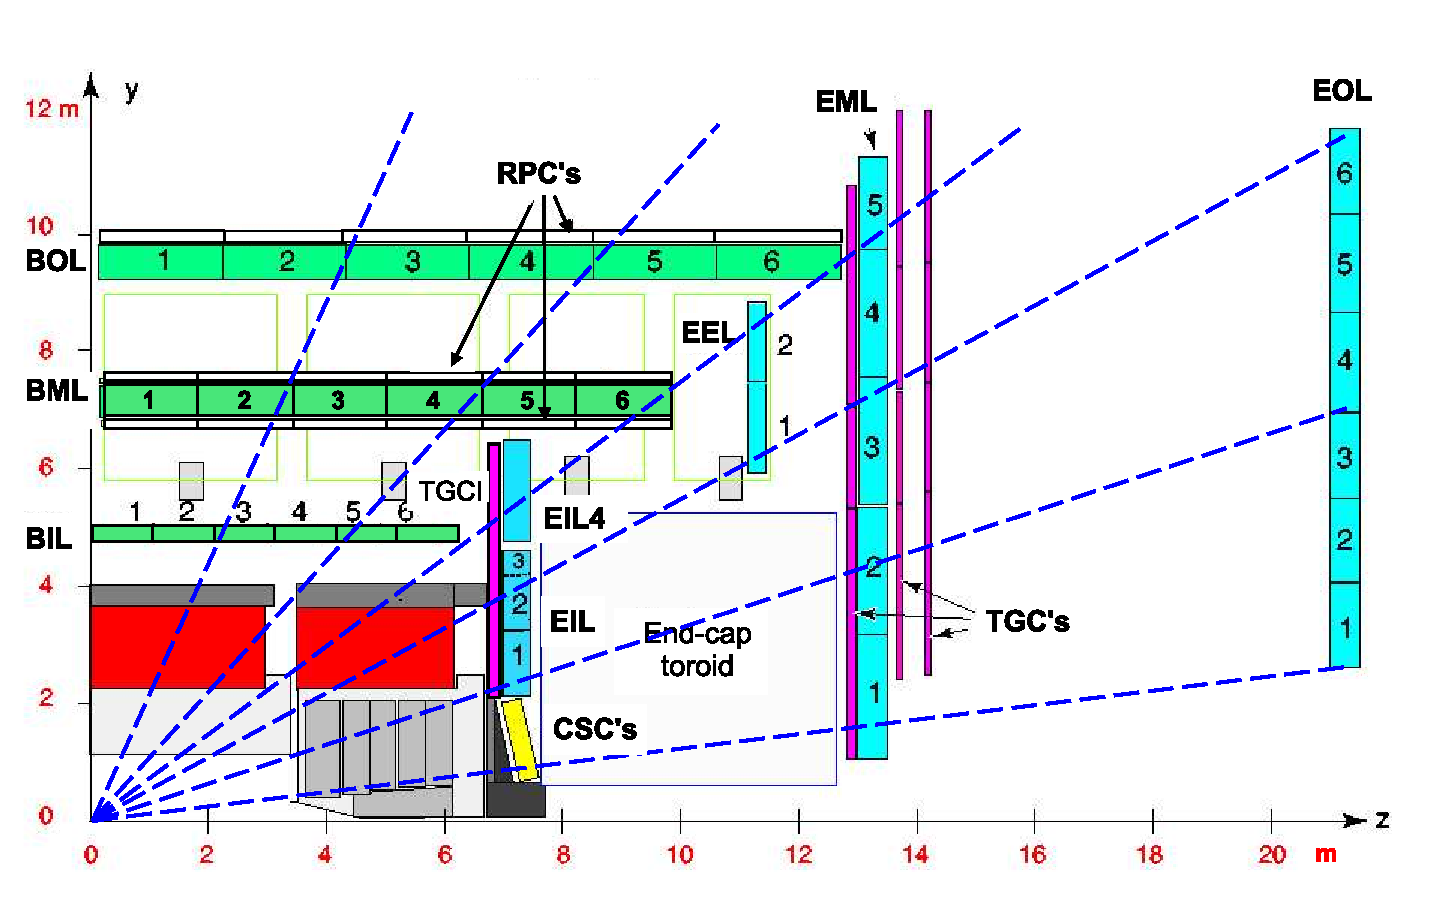
\includegraphics[width=\fullfig]{figures/muon_side_schematic.pdf}
\caption{A quarter view of the muon spectrometer which higlights the layout of each of the detecting elements. The BOL, BML, BIL, EOL, EML, and EIL are all \ac{MDT} elements, where the acronyms encode their positions.}
\label{fig:muon_side_schematic}
\end{figure}

\begin{figure}[hbtp]
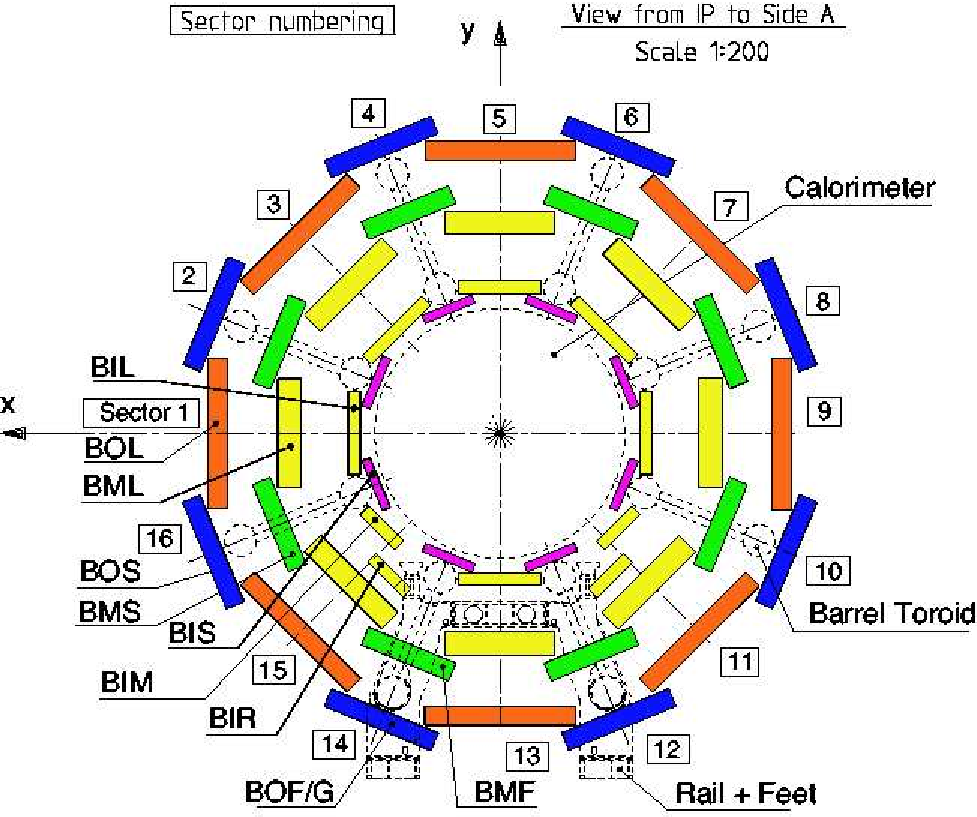
\includegraphics[width=\fullfig]{figures/muon_barrel_schematic.pdf}
\caption{A schematic of the cross-section of the muon spectrometer in the barrel region.}
\label{fig:muon_barrel_schematic}
\end{figure}


\subsection{\acl{MDT}}
\label{sec:mdt}
The momentum measurements in the barrel region are provided by three consectuive layers of \ac{MDT} elements, located at approximately 5 m, 7 m, and 9 m from the interaction point.
Each of these layers is a composite of two multilayers of drift tubes: two layers of three to four layers of tubes, as shown in Figure~\ref{fig:mdt_schematic}.
These aluminum tubes are 3 cm in diamete, with lengths between 0.9 and 6.2 m, and are filled with a mixture of ArCO\tsub{2} kept at 3 bar absolute pressure.
A central tungsten-rhenium wire with a diameter of 50 \um runs along the length of the tube, and is kept at a potential of 3080 V.

\begin{figure}[hbtp]
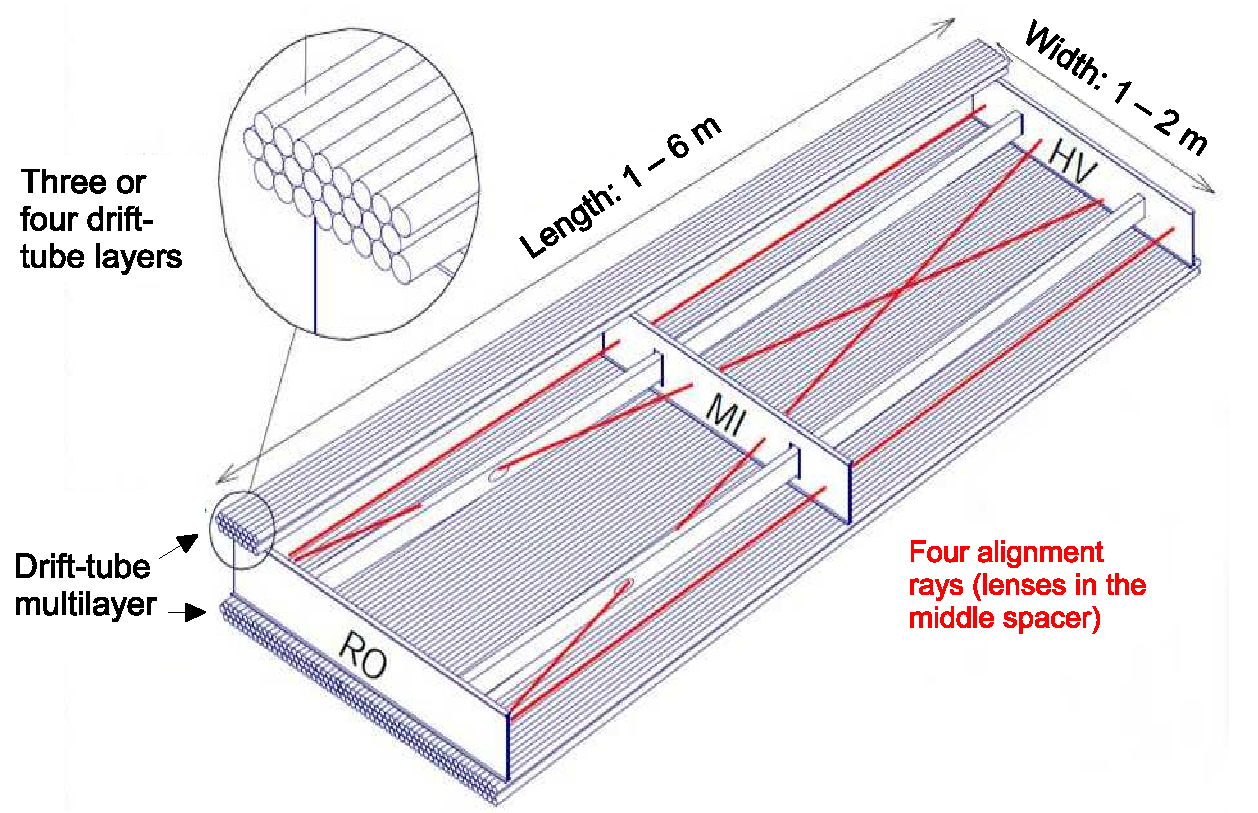
\includegraphics[width=\fullfig]{figures/mdt_schematic.pdf}
\caption{A schematic of a single \ac{MDT} chamber, which shows the multilayers of drift tubes as well as the alignment system.}
\label{fig:mdt_schematic}
\end{figure}

A muon traversing these tubes ionizes the gas, and the ionization electrons then drift in the electric field toward the central wire.
Close to the wire, the electric field is strong enough to cause the original ionization electrons to ionize additional electrons, producing an avalanche that can be measured as a current along the wire. 
The time of arrival of that current depends on how far the muon entered from the wire, and can be used to achieve a position resolution of 80\um in an individual tube.
The combination of the measurements in the consecutive layers of tubes improves this position resolution to 35\um.

To achieve a good resolution over the entire length of a muon track, the relative positions of the tubes of the muon spectrometer must be known to an accuracy of 30\um. 
This is achieved by an optical laser alignment system placed in each of the individual chambers and throughout the cavern.
These monitor any changes in position or alignment due to effects like gravitational sag, temperature shifts, and the magnetic field.
The configuration of the alignment system within an individual chamber is also shown in Figure~\ref{fig:muon_barrel_schema}.

\subsection{\acl{RPC}}

The \ac{RPC} is the outermost detecting layer in the muon spectrometer in the barrel region, and provides a fast measurement of the $\phi$ position of muons for triggering.
The speed of the measurement, with a time resolution of just a few nanoseconds, requires a poor spatial resolution of approximately 1 cm. 
There are three \acp{RPC} layers in the muon spectrometer, two located on either side of the central \ac{MDT} layer and one located outside the final \ac{MDT} layer, as shown in Figure~\ref{fig:muon_side_schematic}.
The \acp{RPC} consist of two layers of parallel plates filled with a gas mixture of C\tsub{2}H\tsub{2}F\tsub{4}.
A muon passing through these systems ionizes the gas, like in the \ac{MDT}, which causes an avalanche of ionization electrons in the electric field maintained between the plates.
Metal strips on the outside of the chamber capacitively couple to the accumulated charge, and are read out to measure the $\eta$ and $\phi$ positions of the muon track. 

\subsection{\acl{CSC}}
The majority of the momentum measurements in the endcap region are provided by the \acp{MDT}.
In the most forward region of the muon spectrometer, between $2.0 < \eta < 2.7$, the particle flux is very high due to contributions from low energy photons and neutrons.
The \ac{MDT} can only sustain a hit rate of approximately 150 Hz/cm\tsup{2} because of limitations in the drift times of the gas and the capacity of the readout electronics. 
The \acp{CSC} were designed to handle higher hit rates, up to 1000 Hz/cm\tsup{2}, and provide the necessary coverage in that high flux region.

The \ac{CSC} consists of several multiwire proportional chambers, where the wires are oriented in the radial direction out from the beampipe.
There are eight large and eight small chambers, arranged to partially overlap in the $\phi$ direction, as shown in Figure~\ref{fig:mcsc_schematic}.
Like in the \ac{MDT}, a muon traversing the system produces ionization in the gas; here, however, the ionization is collected on a number of wires.
These wires couple to cathodes on the chambers which are segmented into strips in two directions.
The relative amount of charge on each of the neighboring strips can be used to interpolate to the position of the muon in both $\eta$ and $\phi$. 

\begin{figure}[hbtp]
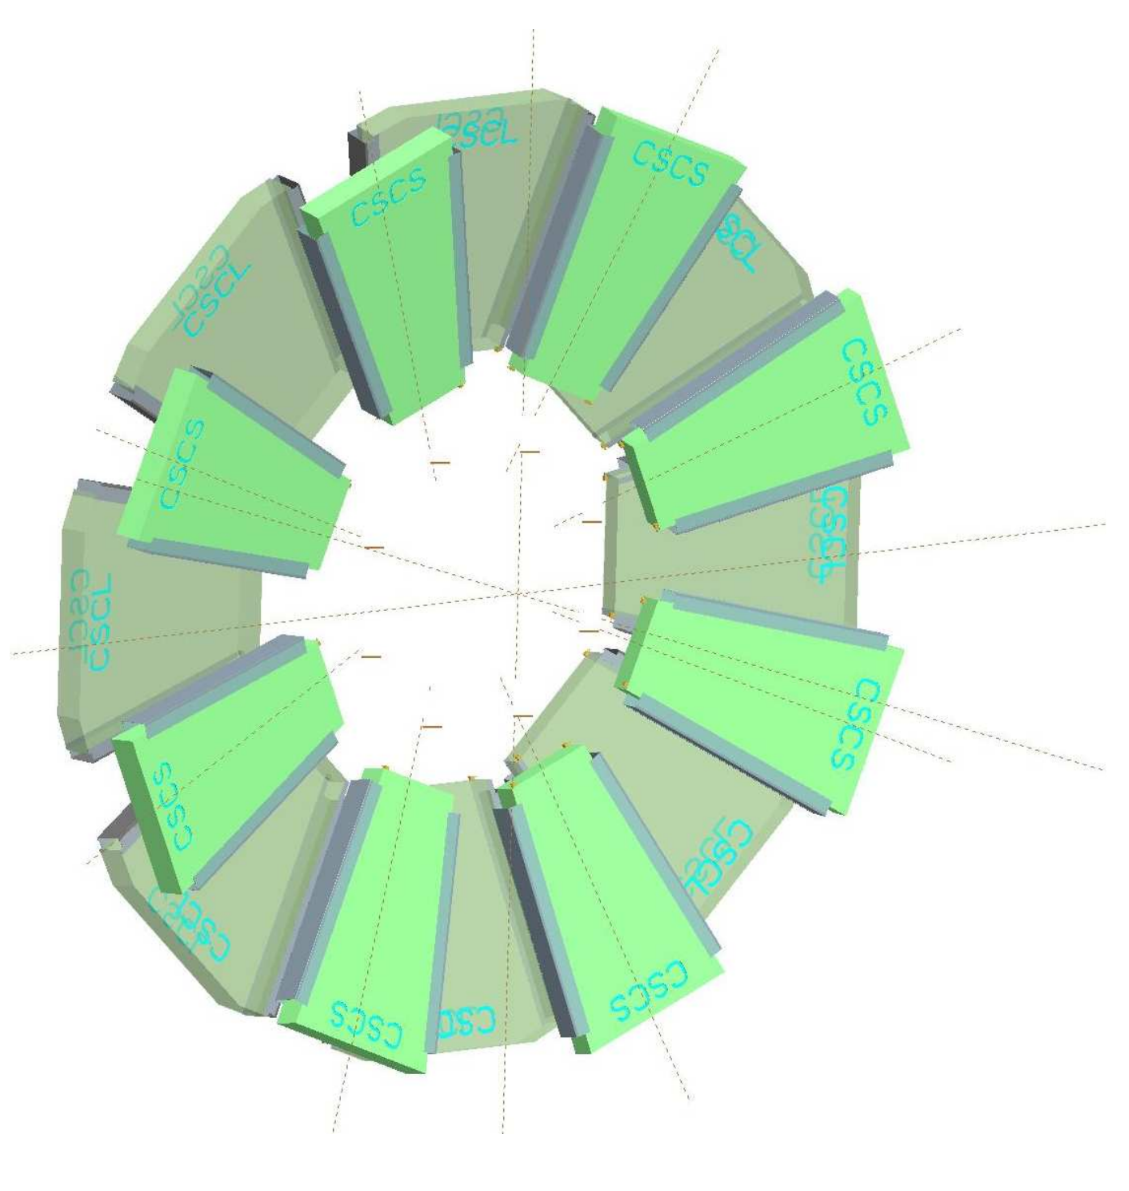
\includegraphics[width=\fullfig]{figures/csc_schematic.png}
\caption{A schematic of the \ac{CSC} endcap, showing the overlapping arrangement of the eight large and eight small chambers.}
\label{fig:csc_schematic}
\end{figure}

\subsection{\acl{TGC}}
Like in the barrel region, a separate, fast detector is required to provide position measurements of muons for trigger in the endcap region.
This is provided by the \ac{TGC} which consists of seven layers in the middle station of the endcap, two doublet layers and one triplet layer, and a single doublet layer in the inner endcap station.
Figure~\ref{fig:tgc_schematic} shows the arrangement of the triple and doublet layers of the \acp{TGC}.

\begin{figure}[hbtp]
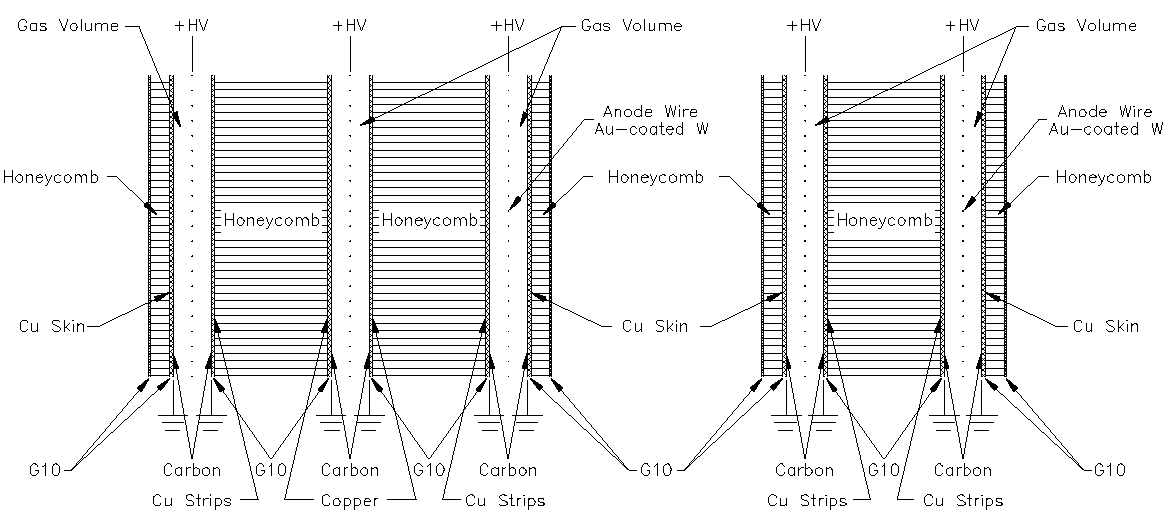
\includegraphics[width=\fullfig]{figures/tgc_schematic.pdf}
\caption{A schematic of the \ac{TGC} doublet and triplet layers.}
\label{fig:tgc_schematic}
\end{figure}

Like the \acp{CSC}s, the \acp{TGC} are multiwire proportional chambers with a wire-to-cathode distance of 1.4 mm and a wire-to-wire distance of 1.8 mm.
Readout strips on the outside of the chambers run perpendicular to the wires, and couple to the charge collected on the wires to provide a position measurement in the $\eta$ direction.
The current induced on the wires is also readout to provide a position measurement in the $\phi$ direction.
The high electric field and small wire-to-wire distance give it the required good time resolution to be used for triggering events. 

% ----------------------------------------

\section{Trigger}
\label{sec:trigger}

It is not possible for the detector and the associated computing systems to record the terabytes of data that the 40 MHz of proton-proton collisions produce every second.
Instead, a small fraction of these events are selected by the trigger system to be recorded and later analyzed.
Selecting interesting events at such a high rate poses a signifcant challenge for the both the detector design and the implementation of a trigger decision and data acquisition system.
The trigger must balance the time needed to decide to keep an event, to avoid losing information, with the filtering accuracy to consistently select a full menu of physics events that can be used for the wide array of searches and measurements targetted by \ac{ATALS}. 

The \ac{ATLAS} trigger system, as of Run 2, consists of two levels of decision making. 
The first level, referred to as L1, is hardware based and uses inputs from a subset of the detector elements to narrow the considered event rate from the original 40 MHz down to 100 kHz.
The 100 kHz rate is the maximal rate that the event information can be transferred from the detector.
The second level, referred to as the \ac{HLT}, makes the final decisions on which events to keep for analysis and selects a rate of around 1 kHz.
The collection of selection criteria used to make the L1 decisions feed into subsequent selection criteria in the \ac{HLT}, and the set of these combinations of L1 and \ac{HLT} critera from the trigger menu which defines exactly what events are recorded on \ac{ATLAS}.
The entirety of the trigger menu used for 2015 data collection is shown in Table~\ref{tab:trigger_menu}, which summarizes the selection requirements at both levels and additionally shows the peak measured rates contributed by each.

\begin{table}[hbtp]
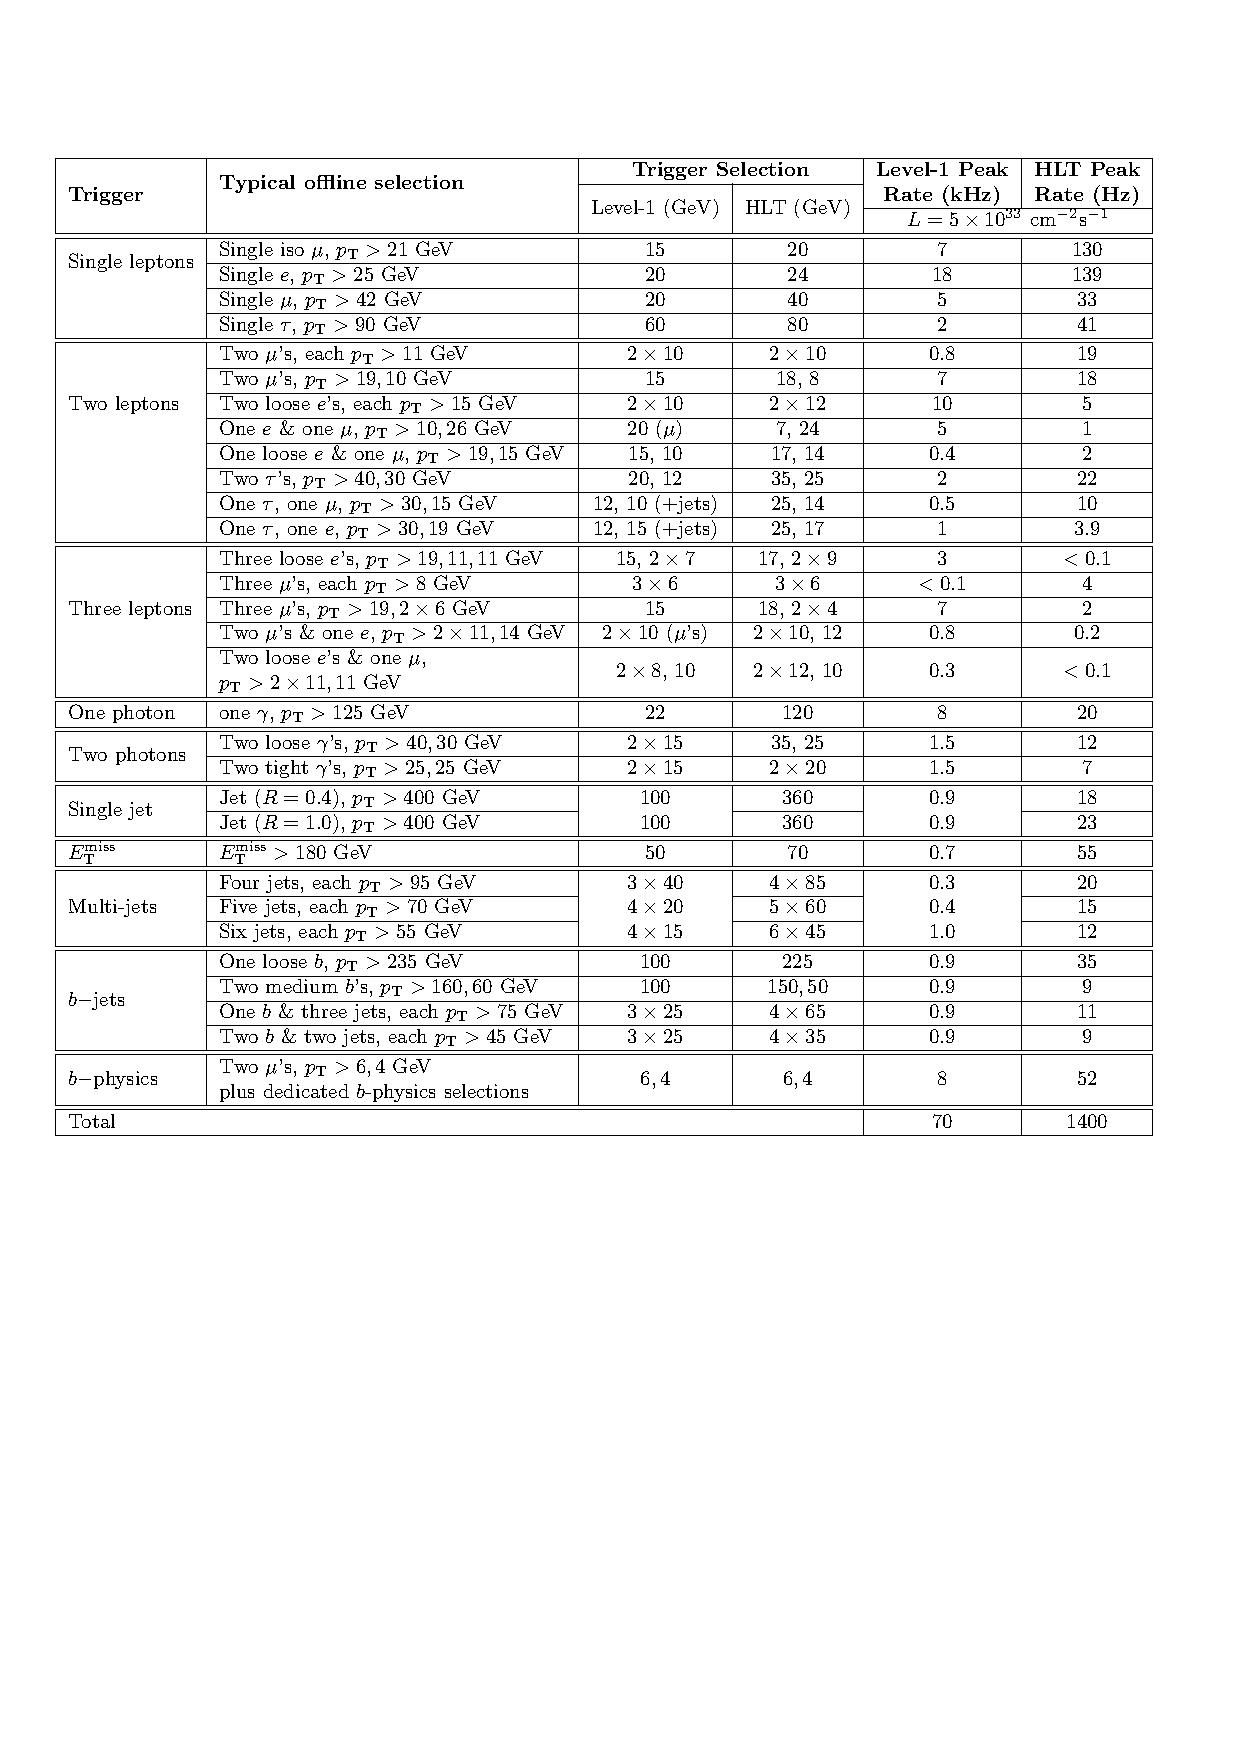
\includegraphics[width=\fullfig]{figures/trigger_menu.pdf}
\caption{The trigger menu for the 2015 data collection with $L = 5 x 10^{33}\lcms$. Both the L1 and \ac{HLT} selection requirements and their trigger rates are shown measured at the specified luminosity are shown. The typical offline selections represent a typical set of offline requirements imposed after the trigger in an analysis.}
\label{tab:trigger_menu}
\end{table}

At L1, the trigger system uses information primarily from the calorimeters and muon spectrometer to select high \pt jets, electrons, photons, and muons. 
The electromagnetic calorimeter uses reduced granularity energy measurements as well as isolation requirements to select electrons and photons.
The hadronic calorimeter also uses a combination of reduced granularity energy measurements and isolation to select high momentum jets and hadronically decaying tau leptons. 
The calorimeters are also used to provide triggers based on missing energy: the coarse granularity energy measurements are used to calculate a directional sum of energies and to trigger on a significant imbalance.
Only the \acp{RPC} and \acp{TGC} muon subdetectors contribute to the decision at L1, and are used to identify high momentum muons.
The contributions to the triggering rate of the various types of L1 triggers are shown in Figure~\ref{fig:trigger_l1rate}. 
The total rate is indicated in black and is lower than the sum of individual rates because their is signifcant overlap between different trigger channels. 
The majority of the rate comes from lepton and photon triggers.

\begin{figure}[hbtp]
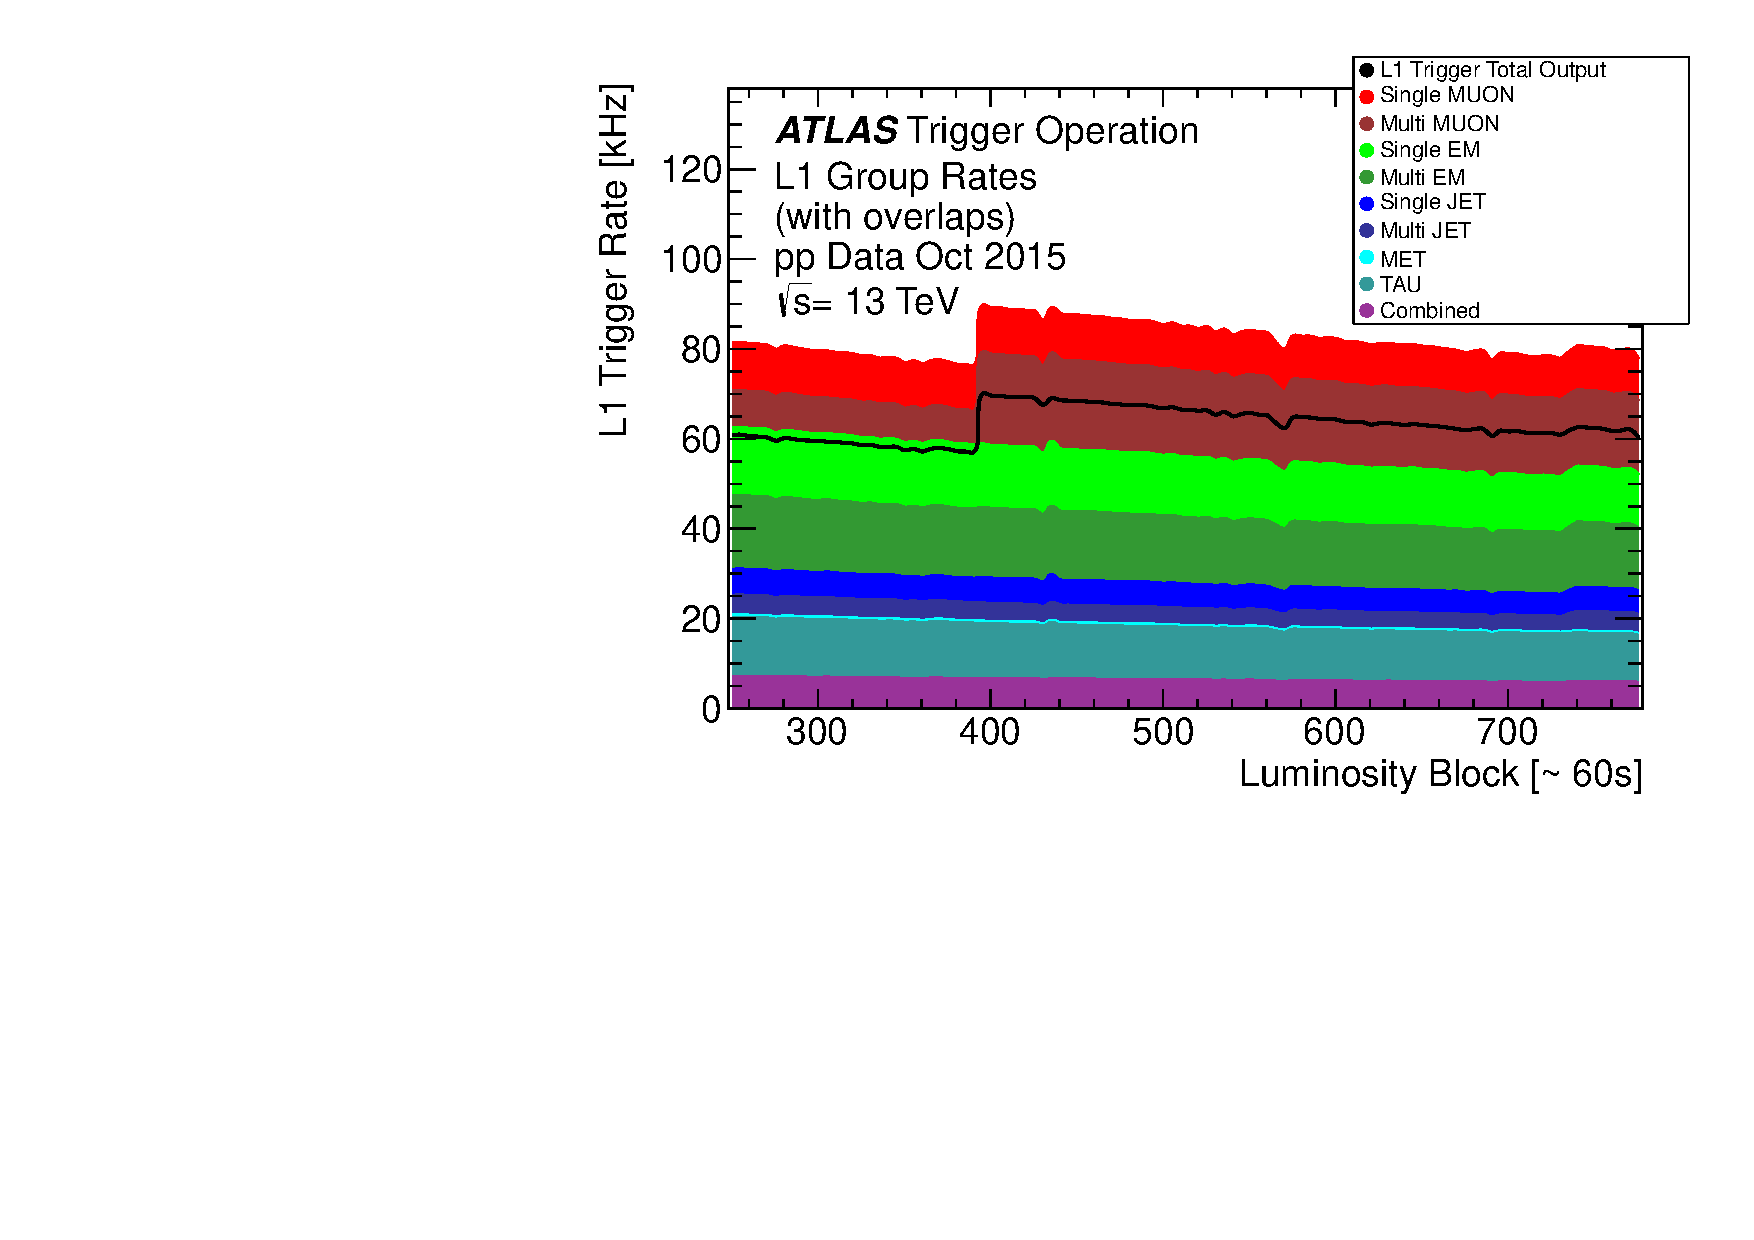
\includegraphics[width=\fullfig]{figures/trigger_l1rate.pdf}
\caption{The L1 Trigger rate broken down into the types of triggers as a function of the luminosity block for the 2015 data collection period.}
\label{fig:trigger_l1rate}
\end{figure}

After an event is chosen by the L1 trigger, the detector measurements from the bunch crossing which fired the trigger is read out from the front-end electronics and stored on read-out boards.
This inclusive information is necessary to make more the more precise event selections than is possible with the reduced information at L1.
The \ac{HLT} then uses this information with software algorithms to decide whether or not to permanently record the event.
The L1 trigger also forwards which decision was made and \acp{RoI} to the \ac{HLT}, which allows the \ac{HLT} to focus on particular algorithms and particular sections of the detector to greatly improve the algorithmic selection speed.
The additional information available to the \ac{HLT} allows it to implement additional trigger targets, such as identified jets from the decays of b-hadrons.
The contributions to the triggering rate of the various types of \ac{HLT} triggers are shown in Figure~\ref{fig:trigger_l1rate}. 

\begin{figure}[hbtp]
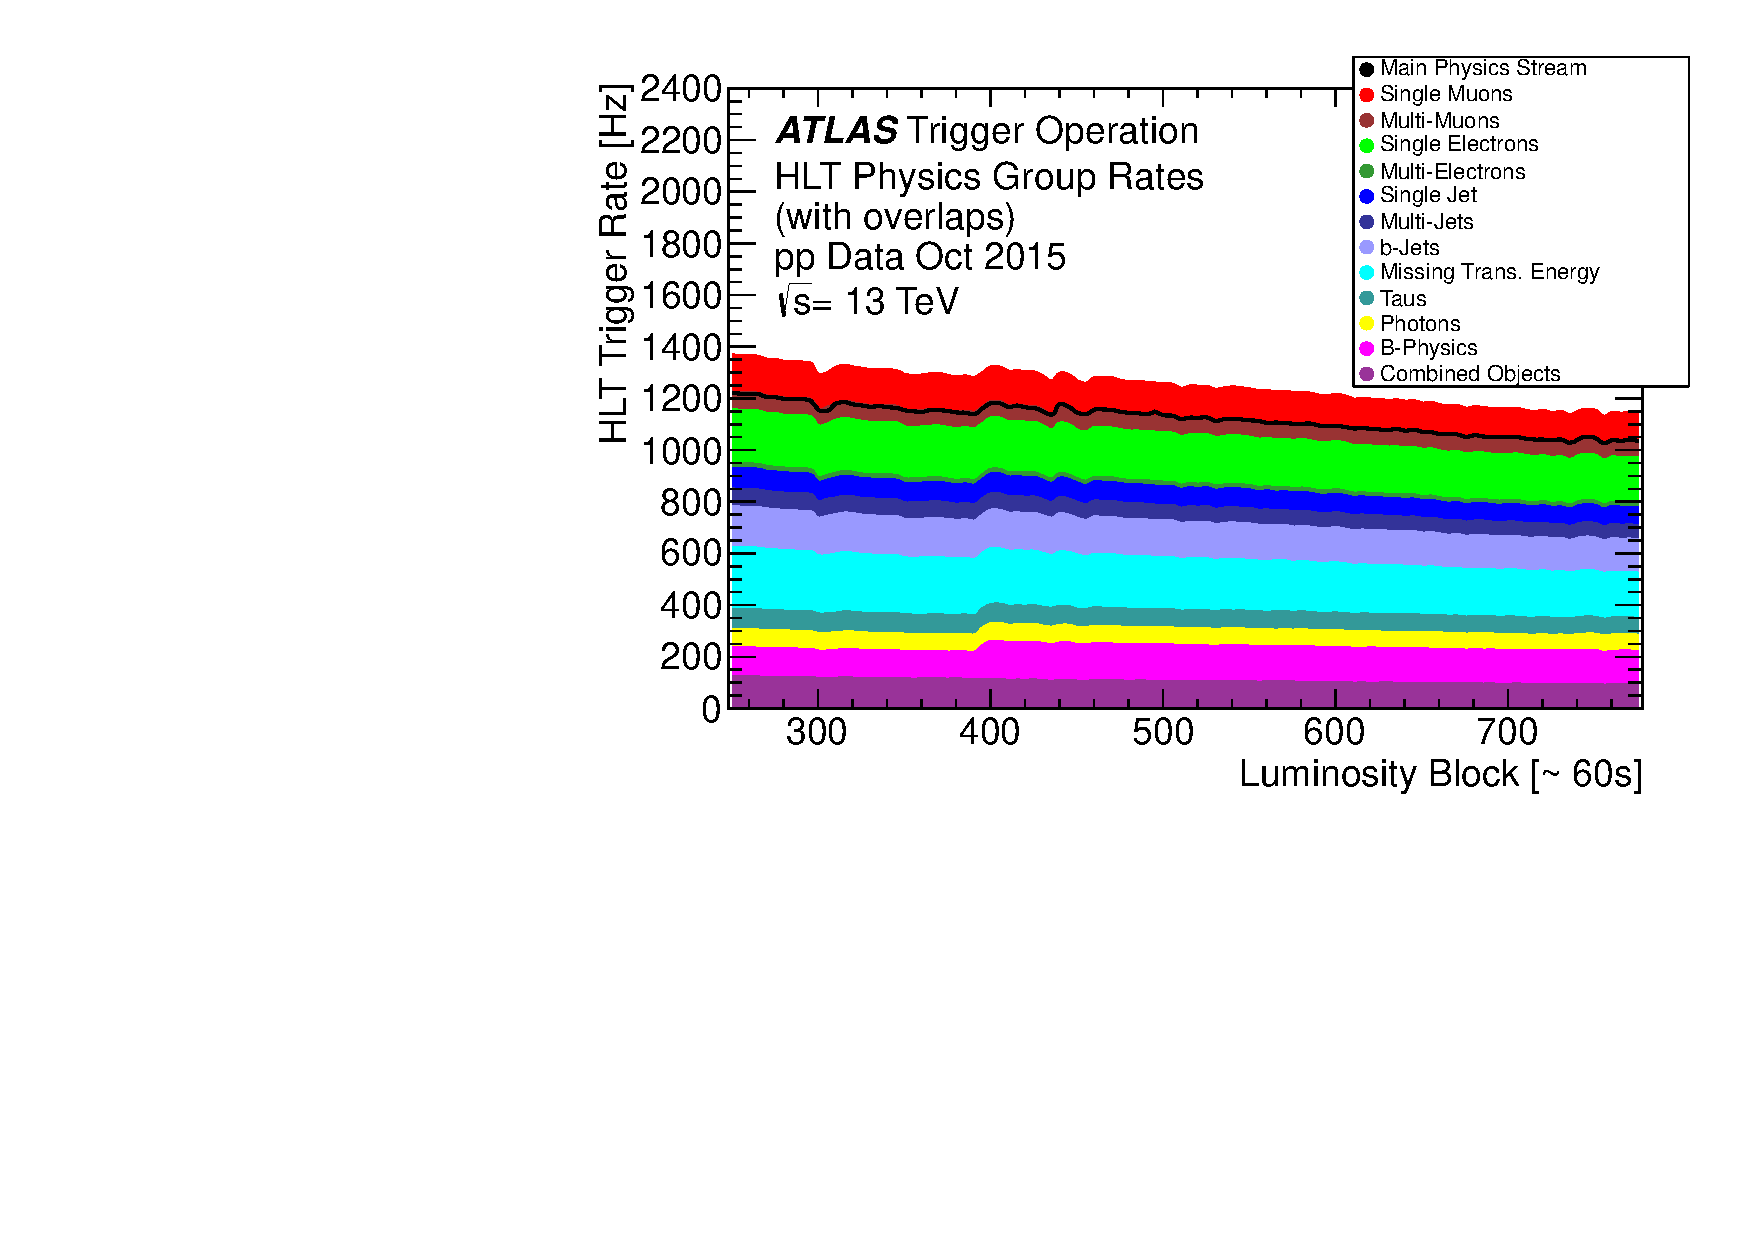
\includegraphics[width=\fullfig]{figures/trigger_hltrate.pdf}
\caption{The HLT Trigger rate broken down into the types of triggers as a function of the luminosity block for the 2015 data collection period.}
\label{fig:trigger_l1rate}
\end{figure}

% ----------------------------------------
